\documentclass[a4paper,11pt]{book}
%\documentclass[a4paper,twoside,11pt,titlepage]{book}

\usepackage[pdftex,dvipsnames]{xcolor}  % Coloured text etc.
\usepackage{xargs}                      % Use more than one optional parameter in a new commands


\usepackage{listings}
\usepackage[utf8]{inputenc}
\usepackage[spanish]{babel}
\usepackage{tcolorbox}
\usepackage{eurosym} % para el euro

%%%%
\usepackage{textcomp}
%\usepackage[style=list, number=none]{glossary} %
%\usepackage{titlesec}
%\usepackage{pailatino}

\decimalpoint
\usepackage{dcolumn}
\newcolumntype{.}{D{.}{\esperiod}{-1}}
\makeatletter
\addto\shorthandsspanish{\let\esperiod\es@period@code}
\makeatother

\usepackage[chapter]{algorithm}
\RequirePackage{verbatim}
%\RequirePackage[Glenn]{fncychap}
\usepackage{fancyhdr}
\usepackage{graphicx}
\usepackage{afterpage}
\usepackage{longtable}
\usepackage[pdfborder={000}]{hyperref} %referencia
\usepackage[toc,page]{appendix}
\usepackage[toc]{glossaries}
\usepackage{subcaption}
\usepackage{multirow}
\usepackage{boldline}
\usepackage{tabularx}
\usepackage{lscape}

% ********************************************************************
% Re-usable information
% ********************************************************************
\newcommand{\myTitle}{Gestión de Funciones de Red Virtuales (NFVs) utilizando OpenStack\xspace}
\newcommand{\myDegree}{Grado en Ingeniería de tecnologías de telecomunicación\xspace}
\newcommand{\myName}{Alejandro Toledo Juan\xspace}
\newcommand{\myProf}{Jorge Navarro Ortiz\xspace}
\newcommand{\myOtherProf}{Nombre Apellido1 Apellido2 (tutor2)\xspace}
%\newcommand{\mySupervisor}{Put name here\xspace}
\newcommand{\myFaculty}{Escuela Técnica Superior de Ingenierías Informática y de
Telecomunicación\xspace}
\newcommand{\myFacultyShort}{E.T.S. de Ingenierías Informática y de
Telecomunicación\xspace}
\newcommand{\myDepartment}{Departamento de teoría de la señal, telemática y comunicaciones...\xspace}
\newcommand{\myUni}{\protect{Universidad de Granada}\xspace}
\newcommand{\myLocation}{Granada\xspace}
\newcommand{\myTime}{\today\xspace}
\newcommand{\myVersion}{Versión 0.1\xspace}


\hypersetup{
pdfauthor = {\myName atj2507@correo.ugr.es},
pdftitle = {\myTitle},
pdfsubject = {},
pdfkeywords = {OpenStack, Cloud, NFVs, VM},
pdfcreator = {},
pdfproducer = {pdflatex}
}

%\hyphenation{}


%\usepackage{doxygen/doxygen}
%\usepackage{pdfpages}
\usepackage{url}

\usepackage{colortbl,longtable}
\usepackage[stable]{footmisc}
\usepackage{index}
\usepackage{pdfpages}
\usepackage{adjustbox}
\usepackage{amsmath}
\usepackage{amssymb}



%%%%
\makeindex
%\usepackage[style=long, cols=2,border=plain,toc=true,number=none]{glossary}
%\makeglossary

%%%%
% Definición de comandos que me son útiles:
\renewcommand{\indexname}{Índice alfabético}
%\renewcommand{\glossaryname}{Glosario}

\pagestyle{fancy}
\fancyhf{}
\fancyhead[LO]{\leftmark}
\fancyhead[RE]{\rightmark}
\fancyhead[RO,LE]{\textbf{\thepage}}
\renewcommand{\chaptermark}[1]{\markboth{\textbf{#1}}{}}
\renewcommand{\sectionmark}[1]{\markright{\textbf{\thesection. #1}}}

\setlength{\headheight}{1.5\headheight}

\newcommand{\HRule}{\rule{\linewidth}{0.5mm}}
%Definimos los tipos teorema, ejemplo y definición podremos usar estos tipos
%simplemente poniendo \begin{teorema} \end{teorema} ...
\newtheorem{teorema}{Teorema}[chapter]
\newtheorem{ejemplo}{Ejemplo}[chapter]
\newtheorem{definicion}{Definición}[chapter]

\definecolor{gray97}{gray}{.97}
\definecolor{gray75}{gray}{.75}
\definecolor{gray45}{gray}{.45}
\definecolor{gray30}{gray}{.94}

\lstset{ frame=Ltb,
     framerule=0.5pt,
     aboveskip=0.5cm,
     framextopmargin=3pt,
     framexbottommargin=3pt,
     framexleftmargin=0.1cm,
     framesep=0pt,
     rulesep=.4pt,
     backgroundcolor=\color{gray97},
     rulesepcolor=\color{black},
     %
     stringstyle=\ttfamily,
     showstringspaces = false,
     basicstyle=\scriptsize\ttfamily,
     commentstyle=\color{gray45},
     keywordstyle=\bfseries,
     %
     numbers=left,
     numbersep=6pt,
     numberstyle=\tiny,
     numberfirstline = false,
     breaklines=true,
   }

% minimizar fragmentado de listados
\lstnewenvironment{listing}[1][]
   {\lstset{#1}\pagebreak[0]}{\pagebreak[0]}

\lstdefinestyle{CodigoC}
   {
	basicstyle=\scriptsize,
	frame=single,
	language=C,
	numbers=left
   }
\lstdefinestyle{CodigoC++}
   {
	basicstyle=\small,
	frame=single,
	backgroundcolor=\color{gray30},
	language=C++,
	numbers=left
   }


\lstdefinestyle{Consola}
   {basicstyle=\scriptsize\bf\ttfamily,
    backgroundcolor=\color{gray30},
    frame=single,
    numbers=none
   }


\newcommand{\bigrule}{\titlerule[0.5mm]}


%Para conseguir que en las páginas en blanco no ponga cabecerass
\makeatletter
\def\clearpage{%
  \ifvmode
    \ifnum \@dbltopnum =\m@ne
      \ifdim \pagetotal <\topskip
        \hbox{}
      \fi
    \fi
  \fi
  \newpage
  \thispagestyle{empty}
  \write\m@ne{}
  \vbox{}
  \penalty -\@Mi
}
\makeatother

\usepackage{pdfpages}
\begin{document}
\begin{titlepage}


\newlength{\centeroffset}
\setlength{\centeroffset}{-0.5\oddsidemargin}
\addtolength{\centeroffset}{0.5\evensidemargin}
\thispagestyle{empty}

\noindent\hspace*{\centeroffset}\begin{minipage}{\textwidth}

\centering

\includegraphics[width=0.9\textwidth]{imagenes/portada/logo_ugr_nuevo.png}\\[1.4cm]

\textsc{ \Large TRABAJO FIN DE GRADO\\[0.2cm]}
\textsc{ GRADO EN INGENIERÍA DE TECNOLOGÍAS DE TELECOMUNICACIÓN}\\[1cm]
% Upper part of the page
%
% Title
{\Huge\bfseries Diseño y despliegue de Funciones de Red Virtuales (VNFs) utilizando OpenStack \\
}
\noindent\rule[-1ex]{\textwidth}{3pt}\\[3.5ex]
%{\large\bfseries Subtitulo del Proyecto}
{\large\bfseries}
\end{minipage}

\vspace{1.6cm}
\noindent\hspace*{\centeroffset}\begin{minipage}{\textwidth}
\centering

\textbf{Autor}\\ { Alejandro Toledo Juan}\\[2.5ex]
\textbf{Director}\\
{Jorge Navarro Ortiz}\\[2cm]
%
\includegraphics[width=0.3\textwidth]{imagenes/portada/etsiit_logo.png}\\[0.1cm]
\textsc{Escuela Técnica Superior de Ingenierías Informática y de Telecomunicación}\\
\textsc{---}\\
Granada, Día Mes de 2018
\end{minipage}
%\addtolength{\textwidth}{\centeroffset}
%\vspace{\stretch{2}}
\end{titlepage}



\chapter*{}
%\thispagestyle{empty}
%\cleardoublepage

%\thispagestyle{empty}

\begin{titlepage}
 
 
\setlength{\centeroffset}{-0.5\oddsidemargin}
\addtolength{\centeroffset}{0.5\evensidemargin}
\thispagestyle{empty}

\noindent\hspace*{\centeroffset}\begin{minipage}{\textwidth}

\centering
%
\includegraphics[width=0.9\textwidth]{imagenes/logo_ugr.jpg}\\[1.4cm]

\textsc{ \Large TRABAJO FIN DE GRADO\\[0.2cm]}
\textsc{ GRADO EN INGENIERÍA DE TECNOLOGÍAS DE TELECOMUNICACIÓN}\\[1cm]
% Upper part of the page
% 

 \vspace{0.3cm}

%si el proyecto tiene logo poner aquí
%
\includegraphics{imagenes/portada/openstack_logo.png} 
 \vspace{0.5cm}

% Title

{\Huge\bfseries Diseño y despliegue de Funciones de Red Virtuales (VNFs) utilizando OpenStack\\
}
\noindent\rule[-1ex]{\textwidth}{3pt}\\[3.5ex]
%{\large\bfseries \\[4cm]}
%{\large\bfseries}
%\end{minipage}

\vspace{0.1cm}
%\noindent\hspace*{\centeroffset}\begin{minipage}{\textwidth}
\centering

\textbf{Autor}\\ {Alejandro Toledo Juan}\\[2.5ex]
\textbf{Director}\\
{Jorge Navarro Ortiz}\\[1.5cm]
%
\includegraphics[width=0.15\textwidth]{imagenes/portada/tstc.png}\\[0.1cm]
\textsc{Departamento de Teoría de la Señal, Telemática y Comunicaciones}\\
\textsc{---}\\
Granada, mes de 201
\end{minipage}
%\addtolength{\textwidth}{\centeroffset}
%\vspace{\stretch{2}}

 
\end{titlepage}






\cleardoublepage
\thispagestyle{empty}

\begin{center}
{\large\bfseries Diseño y despliegue de Funciones de Red Virtuales (VNFs) utilizando OpenStack}\\
\end{center}
\begin{center}
Alejandro Toledo Juan\\
\end{center}

%\vspace{0.7cm}
\noindent{\textbf{Palabras clave}: Cloud, Devstack, Heat, IaaS, IT, NFVs, OpenStack, Tacker, VIM, VNF}\\

\vspace{0.7cm}
\noindent{\textbf{Resumen}}\\

\jorge{Yo introduciría el concepto de nube y su relevancia actual, metiendo algún párrafo que otro. Y después sí comentas qué se hace en este trabajo (los párrafos que has puesto debajo).}
\jorge{Por cierto, puedes usar \textbackslash alejandro\{texto\} para poner comentarios tuyos. Así los distingo rápido (están en verde, los míos en violeta, y los que sean muy importantes en rojo). Te pongo un ejemplo debajo:}
\alejandro{Esto es un ejemplo.}

En este trabajo se pretende realizar la instalación y configuración de un \textit{cloud} basado en el software OpenStack, con el objetivo de ejecutar en el mismo una serie de funciones de red virtualizadas (VNFs). Estas funciones se deberán poder instanciar y gestionar de forma automática.

\jorge{Los términos en inglés ponlos en cursiva, con \textbackslash textit\{texto\}}

Este trabajo busca una visión para profesionales de IT que quieren una descripción general de alto nivel de OpenStack, y que desean saber si OpenStack es la solución adecuada para satisfacer las necesidades de IT de su organización. En él también ayudaremos a cualquier persona que quiera establecer un entorno de prueba OpenStack a pequeña escala a adquirir experiencia trabajando con OpenStack.

\cleardoublepage


\thispagestyle{empty}


\begin{center}
{\large\bfseries Project Title: Design and Dimensioning Virtual Network functions (NFVs) using OpenStack}\\
\end{center}
\begin{center}
Alejandro Toledo Juan\\
\end{center}

%\vspace{0.7cm}
\noindent{\textbf{Keywords}: Cloud, Devstack, Heat, IaaS, IT, NFVs, OpenStack, Tacker, VIM, VNF}\\

\vspace{0.7cm}
\noindent{\textbf{Abstract}}\\

\jorge{Idem, actualiza el resumen en inglés cuando hayas cambiado el resumen en español.}

In this work we intend to perform the installation and configuration of a cloud based on the OpenStack software, in order to execute a series of virtualized network functions (VNFs). These functions should be able to instantiate and manage automatically.

This work seeks a vision for IT professionals who want an
OpenStack general-level description, and know if OpenStack
is the solution for the right one to meet the IT needs of their organization. At the same time we will help anyone
to deploy an OpenStack  small scale test environment to gain experience working with OpenStack.




\chapter*{}
\thispagestyle{empty}

\noindent\rule[-1ex]{\textwidth}{2pt}\\[4.5ex]

Yo, \textbf{Alejandro Toledo Juan}, alumno de la titulación GRADO EN INGENIERÍA DE TECNOLOGÍAS DE TELECOMUNICACIÓN  de la \textbf{Escuela Técnica Superior
de Ingenierías Informática y de Telecomunicación de la Universidad de Granada}, con DNI 71223946F, autorizo la ubicación de la siguiente copia de mi Trabajo Fin de Grado en la biblioteca del centro para que pueda ser consultada por las personas que lo deseen.

\vspace{6cm}

\noindent Fdo: Alejandro Toledo Juan

\vspace{2cm}

\begin{flushright}
Granada a día de mes de 201 .
\end{flushright}


\chapter*{}
\thispagestyle{empty}

\noindent\rule[-1ex]{\textwidth}{2pt}\\[4.5ex]

D. \textbf{Jorge Navarro Ortiz}, Profesor del Área de Ingeniería Telemática del Departamento de Teoría de la Señal, Telemática y Comunicaciones de la Universidad de Granada.

\vspace{0.5cm}


\vspace{0.5cm}

\textbf{Informan:}

\vspace{0.5cm}

Que el presente trabajo, titulado \textit{\textbf{ Gestión de Funciones de Red Virtuales (NFVs) utilizando OpenStack}}, ha sido realizado bajo su supervisión por \textbf{Alejandro Toledo Juan}, y autorizo la defensa de dicho trabajo ante el tribunal que corresponda.

\vspace{0.5cm}

Y para que conste, expiden y firman el presente informe en Granada a X de mes de 201 .

\vspace{1cm}

\textbf{El director:}

\vspace{5cm}

\noindent \textbf{Jorge Navarro Ortiz \ \ \ \ \ }

\chapter*{Agradecimientos}
\thispagestyle{empty}

       \vspace{1cm}


Poner aquí agradecimientos...


%% Esta línea la he puesto yo para el glosario a ver si cuela
%\newglossaryentry{API}
{
    name=API,
    description={Application Programming Interface}
}

\newglossaryentry{CLI}
{
    name=CLI,
    description={Command Line Interface}
}

\newglossaryentry{ETSI}
{
    name=ETSI,
    description={European Telecommunication Standars Institute}
}

\newglossaryentry{IaaS}
{
    name=IaaS,
    description={Infraestructure as a Service}
}

\newglossaryentry{IT}
{
    name=IT,
    description={Information Technology}
}

\newglossaryentry{LVM}
{
    name=LVM,
    description={Linux Volume Manager}
}

\newglossaryentry{NAT}
{
    name=NAT,
    description={Network Address Translation}
}


\newglossaryentry{NFV}
{
    name=NFV,
    description={Network Function Virtualization}
}

\newglossaryentry{NFVI}
{
    name=NFVI,
    description={NFV Infraestructure}
}

\newglossaryentry{NFVO}
{
    name=NFVO,
    description={NFV Orchestrator}
}

\newglossaryentry{NSD}
{
    name=NSD,
    description={Network Services Descriptors}
}


\newglossaryentry{PaaS}
{
    name=PaaS,
    description={Platform as a Service}
}


\newglossaryentry{SaaS}
{
    name=SaaS,
    description={Software as a Service}
}

\newglossaryentry{SDN}
{
    name=SDN,
    description={Software Defined Network}
}


\newglossaryentry{SDS}
{
    name=SaaS,
    description={Software Defined Storage}
}

\newglossaryentry{TIC}
{
    name=TIC,
    description={Tecnologías de Información y comunicación}
}


\newglossaryentry{VIM}
{
    name=VIM,
    description={Virtual Infrastructure Manager}
}


\newglossaryentry{VM}
{
    name=VM,
    description={Virtual Machine}
}


\newglossaryentry{VNF}
{
    name=VNF,
    description={Virtual Network Function}
}

\newglossaryentry{VNFD}
{
    name=VNFD,
    description={VNF Descriptors}
}

\newglossaryentry{VNFFGD}
{
    name=VNFD,
    description={VNF Forwarding Graph Descriptors}
}

\newglossaryentry{VNFM}
{
    name=VNFM,
    description={VNF Manager}
}


\printglossary
\frontmatter
\tableofcontents
\listoffigures
\listoftables


\mainmatter
\setlength{\parskip}{5pt}


\chapter{Introducción} 
\label{chap:introudccion}
En la actualidad los servicios IT han alcanzado un papel crítico en el desarrollo de nuestra sociedad, haciendo que surjan tecnologías como la computación en la nube, la virtualización, o la orquestación de estos elementos virtuales, que ahora marcan el camino a seguir en los despliegues de cualquier infraestructura de red. Dentro de este ámbito, es imprescindible dotar a todos los servicios que existen de mecanismos de gestión y aprovechamiento de los recursos para complacer las demandas de los usuarios asegurando alta disponibilidad.

Este primer capítulo tiene como fin hacer una primera presentación de los aspectos relacionados con el trabajo fin de grado. En primer lugar vamos a describir algunos detalles que nos ayudarán a contextualizar las tecnologías implicadas para, a continuación, exponer las metas que nos proponemos alcanzar a lo largo del desarrollo del mismo.

Hablaremos también de la situación actual de los desarrollos \textit{cloud} basados en OpenStack y la relevancia que tiene en los despliegues en entornos de producción hoy día.

Finalmente, subrayaremos la estructura del resto de la memoria incluyendo la descripción de cada uno de los capítulos y apéndices incluidos en esta memoria.

\section{Contexto y motivación}
\textit{Cloud computing} es un paradigma de computación que permite ofrecer recursos de computación a través de la red. Estos recursos (redes, almacenamiento, cómputo, servidores, aplicaciones, servicios) se ofrecen bajo demanda y pueden ser suministrados con una mínima interacción y gestión por parte del proveedor del servicio.

Este es el punto en el que OpenStack entra en juego. El proyecto OpenStack se define así mismo como una plataforma de cloud computing hecha con software libre para desplegar nubes públicas y privadas orientadas a ofrecer infraestructuras como servicio (\textit{Infrastructure as a Service, IaaS}) a los usuarios, desarrollada con la idea de ser sencilla de implementar, masivamente escalable y con muchas prestaciones.

OpenStack está creciendo a un ritmo sin precedentes. Prueba de ello es el hecho de que el 65\% de las implementaciones de \textit{cloud} en  producción y el 96\% de quienes están llevando acabo despliegues de VNFs (\textit{Virtual Network Functions}) lo usan, convirtiéndose así en una parte esencial de las nuevas infraestructuras de red \cite{noauthor_openstack-annualreport2017.pdf_nodate}. Otra muestra de la relevancia de este proyecto es el hecho de que, según el informe de trabajos de código abierto de \textit{The Linux Foundation and Dice} \cite{foundation_new_2018}, el 64\% de los gerentes de contratación dice que la experiencia con OpenStack y otras tecnologías en la nube están impulsando las decisiones de contratación en trabajos relacionados con el despliegue de infraestructuras de \textit{data centers}, \textit{cloud} y virtualización.

Por tanto, un motivo fundamental a la hora de considerar esta herramienta para el presente trabajo es el creciente uso en despliegues profesionales de tecnologías IT y el papel fundamental que OpenStack tiene hoy día en el desarrollo de despliegues de redes virtuales, gestión de NFV (\textit{Network Fuction Virtualization}), centros de datos, \textit{edge computing}, contenedores y entornos \textit{cloud}.

Otro aspecto importante a la hora de desarrollar el proyecto, es la cantidad de nuevas tecnologías que se pueden usar y con las que se trabaja en este tipo de entornos, conociendo así el alcance que puede llegar a tener OpenStack.

También resulta relevante el cambio de enfoque respecto a los centros de datos convencionales. En el enfoque tradicional de implementación de centros de datos con máquinas físicas existen muchos recursos desaprovechados, en contraposición con el enfoque de computación en la nube, donde los recursos se comparten globalmente permitiendo una mayor elasticidad y reduciendo así costes en espacio y nuevos medios entre otros.

Otro buen motivo para trabajar con esta herramienta es el hecho de que es \textit{Open Source}. OpenStack es una plataforma de \textit{cloud computing} cuyo desarrollo se basa en Licencia Apache 2.0 \cite{noauthor_open_nodate}, una licencia libre que nos permite acceder al código fuente y modificarlo o realizar aportaciones y que además no hace uso de funcionalidades de pago.

\section{Objetivos y alcance del proyecto}

\begin{tcolorbox}[colback=red!5!white,colframe=red!75!black]
% * <atj.itt@gmail.com> 2018-09-02T17:17:57.771Z:
% 
% aa
% 
% ^ <atj.itt@gmail.com> 2018-09-02T17:18:07.122Z.
\begin{itemize}
\item Indicar alcance de cada objetivo.
\item Indicar las interdependencias entre los objetivos y también enlazarlos con los diferentes apartados de la memoria.
\item Destacar aspectos formativos previos más utilizados en este apartado.
\item ¿Es conveniente listar en puntos objetivos o se entiende de este modo lo que se trata de conseguir?
\end{itemize}

\end{tcolorbox}

\begin{tcolorbox}[colback=orange!5!white,colframe=orange!75!black]
Jorge: IMPORTANTE. Como dices en el cuadro, debes expresar claramente los objetivos. Queremos crear una nube que pueda orquestar funciones de red virtuales, de forma que si una se cae, se levante en otro sitio automáticamente. Este es el objetivo principal. Y después, desarrolla los subobjetivos que veas.
\end{tcolorbox}

El proyecto actual se lleva acabo como reto personal en el que se pretende conseguir crear un entorno de \textit{cloud} privado preparado para implementar en un futuro cualquier servicio que se quisiera dar, dotando a la infraestructura de mecanismos de orquestación, escalabilidad y redundancia de funciones de red y recursos, de modo que aseguremos alta disponibilidad frente a catástrofes como puedan ser terremotos, incendios, cortes de luz o fallos en el sistema de cualquier otra índole.

En primer lugar, comenzaremos haciendo un repaso de las tecnologías y conceptos implicados en la realización del presente trabajo y también de nociones varias que nos ayudarán a comprender el alcance que puede llegar a tener el uso de OpenStack.

Pasaremos después a ver las distintas opciones o herramientas similares que tenemos a la hora de desplegar nuestro entorno de trabajo. Una vez seleccionadas las opciones oportunas que iremos viendo y justificando, realizaremos el despliegue de nuestra infraestructura.

Antes de realizar dicho despliegue, será importante hacer una planificación exhaustiva tanto de los recursos hardware, software y otros posibles que puedan estar implicados así como de los costes que conllevan.

Con todo ello, plantearemos el diseño de la infraestructura razonando los motivos que nos han llevado a optar por esa vía para a continuación realizar la instalación de la misma.

\jorge{Ten cuidado cuando usas ''implementar''. Desplegar OpenStack puede ser instalar, configurar, desplegar, ... pero implementar me suena más a crear código. En el caso de los escenarios sí los has implementado, porque tú has escrito los scripts (o a través del GUI) para generarlos, no es una mera instalación y configuración.}

Una vez este a punto nuestra infraestructura, veremos como podemos realizar la gestión de la plataforma para crear nuestra \textit{cloud} privada tanto vía web con la ayuda de uno de los proyectos de OpenStack, como desde línea de comandos y de manera automatizada, creando redes, cortafuegos, máquinas virtuales y asignando recursos a estas máquinas entre otras posibilidades que nos permitirán sacarle el máximo partido a los escenarios creados.

Una vez creados los escenarios, veremos distintos métodos para realizar la gestión de algunas funciones de red, de forma que aseguremos la disponibilidad de las instancias creadas en nuestra nube.

\jorge{Yo quizá contaría aquí qué escenarios quieres crear y con qué objetivo. Has escrito una descripción de lo que has hecho, más a modo de diario que de definición de objetivos. Revísalo y mira si puedes poner más claramente los objetivos.}

\section{Estructura de la memoria} \label{subchap:estrucutramemoria}

Este documento consta de nueve capítulos que describimos a continuación:

\begin{itemize}
\item \textbf{Capítulo \ref{chap:introudccion}: Introducción}. Breve explicación del contexto y las razones de llevar a cabo este proyecto así como los objetivos a alcanzar.
\end{itemize}

\begin{itemize}
\item \textbf{Capítulo \ref{chap:conceptos previos}: Conceptos previos}. En este capítulo se abordarán conceptos y tecnologías relacionadas con las posibilidades que OpenStack ofrece haciendo énfasis en aquellas que atañen a este proyecto.
\end{itemize}

\begin{itemize}
\item \textbf{Capítulo \ref{chap:estadodelarte}: Estado del arte}. Exploración de las principales soluciones del mercado que existen como alternativa y justificación de la elección.
\end{itemize}

\begin{itemize}
\item \textbf{Capítulo \ref{chap:planificacionycostes}: Planificación y costes}. Estimación del tiempo, recursos empleados y costes asociados para llevar a cabo el proyecto.
\end{itemize}

\begin{itemize}
\item \textbf{Capítulo \ref{chap:herramientasutilizadas}: Herramientas utilizadas}. Análisis en profundidad de OpenStack y los principales proyectos que lo componen haciendo énfasis en aquellos que usaremos.
\end{itemize}

\begin{itemize}
\item \textbf{Capítulo \ref{chap:diseno}: Diseño}. Explicación y justificación de los distintos escenarios planteados para la orquestación de las funciones de red.
\end{itemize}

\begin{itemize}
\item \textbf{Capítulo \ref{chap:implementacion}: Implementación}. Documentación del proceso seguido para la instalación de la infraestructura y la puesta a punto de los distintos escenarios y servicios planteados.
\end{itemize}

\begin{itemize}
\item \textbf{Capítulo \ref{chap:pruebas}: Pruebas y resultados}. Realización de diferentes test para corroborar el correcto funcionamiento del despliegue realizado.
\end{itemize}

\begin{itemize}
\item \textbf{Capítulo \ref{chap:conclusiones}: Conclusiones y líneas futuras}. Culminación de la memoria haciendo y repaso de los objetivos alcanzados y prospección de futuras vías para la ampliación del trabajo.
\end{itemize}

Al final de la memoria, podremos encontrar además distintos apéndices:

\begin{itemize}
\item \textbf{Apéndice \ref{chap:arquitectura}: Arquitectura lógica de OpenStack}. Arquitectura lógica en la que se muestran los componentes de los principales proyectos de OpenStack y la relación que hay entre ellos.
\end{itemize}

\begin{itemize}
\item \textbf{Apéndice \ref{chap:manualdeinstalacion}: Archivos de configuración para la instalación}. El proceso de instalación de OpenStack con DevStack tiene como elemento principal un archivo de configuración donse se describen los recursos que queremos que tenga nuestra nube. Este tema merece una mención especial y se propone como anexo al proceso de instalación que se verá en la sección \ref{sec:instalacion}.
\end{itemize}

\begin{itemize}
\item \textbf{Apéndice \ref{chap:creacionescenariobash}: Creación de un escenario mediante scripting en bash}. Generación de un script para automatizar la tarea de configurar un escenario de red desde la línea de comandos.
\end{itemize}







\chapter{Conceptos previos} 
\label{chap:conceptos previos}
Este capítulo trata de recoger y exponer los principales conceptos y tecnologías implicadas en los despliegues en los que se usa Openstack.

Para ello iremos desde el concepto de virtualización hasta llegar al cloud computing, pasando por la tecnología de contenedores a la par que analizamos los beneficios de estos y algunos inconvenientes para acabar hablando de la virtualización de funciones de red o NFV y el rol que OpenStack tiene en ella.

\section{De la virtualización al Cloud Computing}

A lo largo de los años, la informática corporativa ha visto muchos desarrollos que han derivado en el aumento de la computación en la nube tal como la conocemos:

\begin{itemize}
\item En la década de 1990, la informática corporativa se centraba en servidores en un centro de datos.
\item En la década de 2000, la informática corporativa se basaba principalmente en la virtualización.
\item En la década de 2010, estamos viendo el aumento de la computación en la nube para aprovechar la informática corporativa.
\end{itemize}

\subsection{Virtualización}
Para introducir los contenidos que trataremos, vamos a hablar en primer lugar de qué es la virtualización. Cuando se habla de virtualización, la mayoría de las personas piensa en máquinas virtuales. Una máquina virtual \textit{(Virtual Machine, VM)} es una computadora en la que el software, así como el hardware, se crean como una solución de software que simula un sistema de computación  y puede ejecutar programas como si fuese una computadora real. El objetivo de la virtualización es proporcionar una versión virtual, en lugar de física, de los activos de TI esenciales:

\jorge{RECOMENDACIÓN: Usa dos apóstrofes en vez de comillas, porque en LaTeX da menos problemas (depende de dónde escribas las comillas generan errores). Y se usa itemize para meter dentro todos los items, no pongas un itemize para cada item. Te comento esto por los errores que pueda darte. Si no hay errores y quieres dejarlo como está, perfecto.}

\begin{itemize}
\item 
\textbf{Hardware}: Este es el uso ''tradicional'', donde el sistema operativo se instala en una representación de software de los recursos de hardware.
\item 
\textbf{Almacenamiento}: También conocido como almacenamiento definido por software (\textit{Software Defined Storage, SDS}). En SDS, se crea una capa entre los discos duros reales y las computadoras que acceden a estos discos duros, con el 	objetivo de hacerlos más accesibles.
\item 
\textbf{Redes}:	Las actuales redes definidas por software (\textit{Software Defined Networks, SDN}). En SDN, los usuarios de la nube pueden crear una infraestructura de red lógica en la parte superior de la red física, lo que hace que sea más fácil satisfacer sus necesidades.
\end{itemize}


\subsection{Beneficios de la virtualización}
En OpenStack, se utilizan todos los tipos de virtualización. La virtualización tiene muchos beneficios para las IT modernas:

\begin{itemize}
\item 
Permite un uso más eficiente de la capacidad del servidor físico. Si se observa la utilización típica de la CPU de los servidores de hardware, lo más probable es que veamos una utilización de CPU inferior al 10 o incluso al 5\%. La virtualización permite ejecutar diferentes máquinas virtuales sobre CPUs físicas, lo que significa que el uso de la CPU se puede optimizar para colocarnos en torno al 80\%.
\end{itemize}

\begin{itemize}
\item 
Permite un uso más eficiente del espacio físico destinado al centro de datos. Este es un gran problema porque el espacio del centro de datos es caro. Imaginemos que deseamos construir un centro de datos en el medio de una gran ciudad. Los metros cuadrados en las grandes ciudades en general son muy caros. Y esa es la razón por la cual la virtualización ayuda en este sentido, porque el uso de máquinas virtuales significa que necesitaremos menos hardware físico, y usar menos hardware físico significa usar menos metros cuadrados con el consecuente ahorro económico. 
\end{itemize}

\begin{itemize}
\item 
Permite un consumo de energía más eficiente. Como resultado de lo anterior, también podremos usar la energía de una manera más eficiente, si pensamos en las facturas de electricidad de los centros de datos corporativos grandes, que pueden llegar a millones. Por tanto, si optimizamos los servidores reduciendo a la mitad la cantidad de servidores físicos que se necesitan, mejoraremos en esto aspecto, utilizando así la mitad de la energía necesaria para ejecutar estos servidores, lo que permite a las compañías ahorrar una gran suma.
\end{itemize}


\subsection{Implicaciones de la Virtualización}
Cuando se trata de virtualización, los activos físicos están representados por software:
\begin{itemize}
\item 
Los servidores y las estaciones de trabajo se están convirtiendo en máquinas virtuales.
\end{itemize}
\begin{itemize}
\item 
Las redes y el almacenamiento también se pueden virtualizar, convirtiéndose así en SDN y SDS.
\end{itemize}
\begin{itemize}
\item 
Con todos estos tipos de virtualización, un administrador puede construir un \textit{data center} definido por software.
\end{itemize}

\subsection{Limitaciones de la virtualización}
Aún así, la virtualización también tiene algunas limitaciones:
\begin{itemize}
\item 
La ausencia de soluciones de autoservicio. En virtualización, es el administrador quien proporciona la infraestructura que está creando el almacenamiento, la red y las máquinas virtuales. Como usuario final, solo se podrá solicitar la virtualización de los recursos para a continuación esperar a que el administrador tenga tiempo para cumplir con esta solicitud.
\end{itemize}
\begin{itemize}
\item 
Escalabilidad limitada. Por supuesto, hay escalabilidad, porque se pueden agregar servidores a la virtualización para alojar más máquinas virtuales, y también se pueden agregar redes, así como almacenamiento. Pero el hecho de que sea el administrador el encargado de estas tareas, hace que la escalabilidad se encuentre restringida. 
\end{itemize}
\begin{itemize}
\item 
La virtualización es relativamente pesada, ya que cada VM tiene su propio kernel. Si estamos ejecutando veinte máquinas virtuales en un \textit{host} de hipervisor, estamos ejecutando veinte kernels diferentes. Si se necesitan, sin embargo, máquinas virtuales con diferentes sistemas operativos, no hay realmente otra solución para hacerlo de manera más eficiente. Por el contrario, si estamos ejecutando sistemas operativos similares, podemos hacerlo de manera más eficiente, y ese es exactamente el objeto de la tecnología de contenedores.
\end{itemize}

\jorge{¿Qué quieres decir con ''un host de hipervisor''? ¿Sería ''un host que actúa como hipervisor''?}

\subsection{Virtualización basada en host vs basada en hipervisor}

La solución más común utilizada para ejecutar máquinas virtuales sobre Linux en un centro de datos es KVM \textit{ (Kernel-based Virtual Machine)}. KVM es un tipo de virtualización basada en hipervisor (como es el caso de otras soluciones como \textit{VMware ESXi}). Cuando se trata de  virtualización basada en hipervisor, la máquina virtual se ejecuta sobre un kernel de virtualización pequeño y altamente optimizado, que permite a la máquina virtual abordar el hardware de manera más eficiente tal como se esquematiza en la parte izquierda de la Fig.\ref{Container vs VM}.

Otra solución de virtualización común es \textit{VirtualBox} (basada en \textit{host}). VirtualBox permite a los desarrolladores ejecutar un sistema operativo virtual en la parte superior de su escritorio. Sin embargo, esta solución no es tan eficiente como la virtualización basada en hipervisor.

\jorge{Yo pondría una descripción un poco más técnica del caso de virtualización basada en host. Entiendo que te refieres a que se utiliza un kernel de propósito general, como el que se encuentra en las distribuciones de Linux, y por tanto no está tan optimizado...}

En el caso de la infraestructura como servicio, las soluciones actuales utilizan virtualización basada en hipervisor.

\subsection{Tecnología de contenedores}
Como solución al problema del peso de la virtualización, surgió la tecnología de contenedores. En IT, el objetivo fundamental es ejecutar una aplicación, y no una máquina virtual. Al fin y al cabo, es el usuario de la aplicación quien tiene una necesidad. Esta necesidad es ejecutar una aplicación, y ningún usuario pedirá, por lo general, una máquina virtual (aunque actualmente existen empresas que están desplegando precisamente este tipo de servicios). Ese es, pues, uno de los principales objetivos de diseño de la tecnología de contenedores.

\begin{figure}
    \centering
    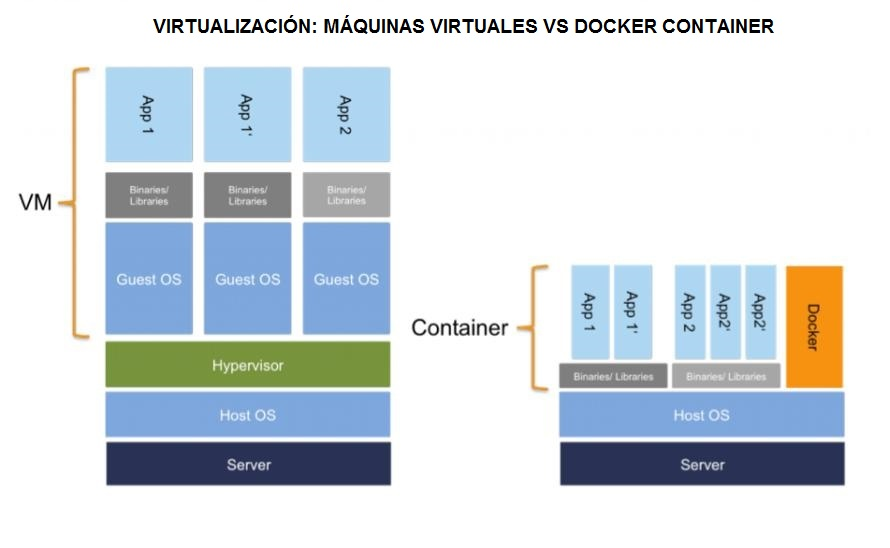
\includegraphics[width=1\textwidth]{imagenes/capitulo1/docker-vm-container.png}
    \caption{Containers vs VMs.}
	\vspace{0.3cm}
    \footnotesize{Fuente: Crisp Research, “Container-Technologien auf dem Vormarsch: Docker in a Nutshell”, 2014}
    \label{Container vs VM}
\end{figure}

Un contenedor es un método de virtualización en el nivel del sistema operativo. Esto permite que varias instancias de un sistema operativo se ejecuten en el mismo kernel, lo que permite un uso más eficiente de los recursos disponibles.

Usar contenedores  facilita a los usuarios finales ejecutar aplicaciones en diferentes plataformas. Las tecnologías de contenedores, como \textit{Docker}, eliminan la necesidad de considerar las diferentes características de la plataforma. El contenedor simplemente se ejecuta como un entorno aislado en la parte superior de la plataforma. Todo lo específico de la aplicación se incluye en un paquete que se ejecuta en la parte superior de cualquier plataforma de hardware. Esto permite al desarrollador centrarse en la aplicación, no en la plataforma subyacente.

Por  tanto, el desafío dentro de un entorno de IT moderno típico es el hecho de la existencia de una gran cantidad de entornos de hardware y multitud de stacks o pilas que necesitan soporte. Cuando hablamos de una pila  o stack, estamos hablando de un entorno completo que se usa para abrir los contenedores, como se puede ver a la derecha de la Fig. \ref{Container vs VM} en comparación de la pila usada para las máquinas virtuales que vemos en la izquierda. 

\begin{figure}
    \centering
    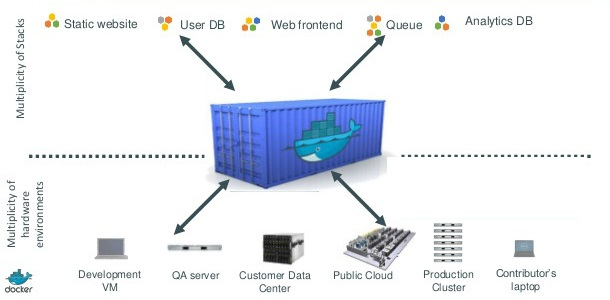
\includegraphics[width=1\textwidth]{imagenes/capitulo1/docker-stacks.png}
    \caption{Docker stacks.}
	\vspace{0.3cm}
    \footnotesize{Fuente: Docker }
    \label{Docker stacks}
\end{figure}

Algunas pilas existentes se ilustran en la Fig.\ref{Docker stacks}, como un sitio web estático, una base de datos de usuario (\textit{user DB}), una interfaz web, una cola o una base de datos de análisis \textit{(analytics BD}). Estas pilas son más que sólo la aplicación, hay un entorno completo que se necesita para ejecutar la pila en la parte superior de un sistema operativo. El propósito de la contenerización es ponerlo todo en un contenedor, de forma que creamos un paquete autónomo donde todo está incluido con el fin de poder ser manipulado usando operaciones estándar y ejecutarse consistentemente en prácticamente cualquier plataforma de hardware como puede ser una VM, un servidor de QA (\textit{Quality Assurance}), un centro de datos de clientes, una nube pública, un \textit{cluster} de producción, una PC portátil, etc.

Por lo tanto, al trabajar con contenedores, los desarrolladores de aplicaciones pueden eliminar los problemas relacionados con la ejecución de aplicaciones sobre diferentes sistemas operativos.

De esta forma, en general, la tecnología de contenedores está haciendo que las IT sean más eficientes.

\begin{itemize}
\item Se pueden implementar fácilmente muchas instancias de una aplicación para que se ejecute sobre un kernel único.
\item Este kernel proporciona entornos aislados y, por lo tanto, seguros.
\item A su vez, esto hace que los contenedores en ejecución sean un proceso seguro: un usuario de un contenedor no puede acceder a los recursos que están asignados a otro contenedor. 
\item Debido al hecho de que muchos contenedores se pueden usar sobre el mismo kernel, los recursos se pueden usar de una manera más eficiente. 
\item La implementación es mucho más llevadera debido al tamaño relativamente pequeño de los contenedores.
\end{itemize}

¿Cuáles son por tanto las diferencias entre los contenedores y la virtualización? Básicamente que los contenedores y la virtualización se utilizan en diferentes contextos:

\begin{itemize}
\item Usaremos contenedores si queremos ejecutar múltiples copias de una sola aplicación, con lo que podremos balancear la carga. 
\item Por otro lado, usaremos máquinas virtuales si necesitamos la flexibilidad de ejecutar múltiples aplicaciones o si queremos poder ejecutarlas en cualquier sistema operativo.
\end{itemize}

Tanto los contenedores como las máquinas virtuales se pueden ejecutar juntos en una nube IaaS.

\section{Cloud Computing}
La computación en la nube o \textit{Cloud Computing}, es un tipo de computación basada en Internet que proporciona recursos de procesamiento compartido y datos a computadoras y otros dispositivos bajo demanda. Permite el acceso bajo demanda a un grupo compartido de recursos informáticos, como redes, servidores, almacenamiento, aplicaciones y servicios, que normalmente están alojados en centros de datos de terceros. La computación en la nube es una metáfora para hacer referencia a un concepto. Para un usuario, los elementos de red que representan los servicios prestados por el proveedor son invisibles, como oscurecidos por una nube. La conclusión es que, desde la perspectiva del usuario, realmente no importa qué recursos se ejecutan o dónde, todo lo que importa son los recursos mismos.

OpenStack pertenece a la categoría de\textit{ computación en la nube IaaS}. Sin embargo, OpenStack evoluciona continuamente, ampliando su alcance. En ocasiones, el enfoque de OpenStack va más allá de IaaS.
Vamos a profundizar más sobre IaaS en cloud y los diferentes tipos de cloud.

\subsection{Tipos de cloud computing}

\begin{figure}[!ht]  \centering
    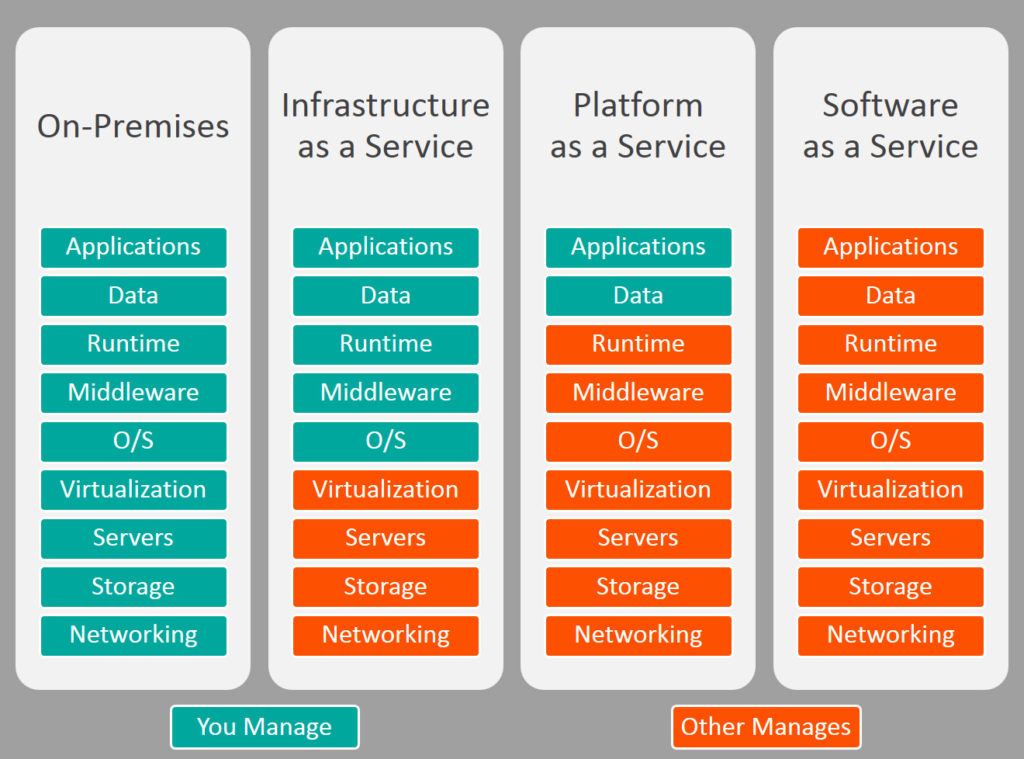
\includegraphics[width=1\textwidth]{imagenes/capitulo1/iaas-paas-saas-comparison.png}
    \caption{Clasificación de cloud computing en base a los recursos que se gestionan.}
	\vspace{0.3cm}
    \footnotesize{Fuente: Stephen Watts, “SaaS vs PaaS vs IaaS: What’s The Difference and How To Choose”, bmc blogs, 2017}    
    \label{comparacion-cloud}
\end{figure}

El concepto de \textit{computación en la nube} es muy amplio, hasta el punto de que podemos afirmar que no existe tal cosa como la computación en la nube. Si le pide a un usuario final que explique qué es la computación en la nube y luego le hace la misma pregunta al administrador del sistema, obtendremos dos descripciones diferentes. En general, hay tres enfoques importantes cuando se trata de computación en la nube dependiendo de los tipos de recursos que se gestionen. En la Fig.\ref{comparacion-cloud} se puede ver esta clasificación tomando como referencia un despliegue tradicional donde se gestionan todos los recursos. Otro punto de vista que lleva a la misma división es, de acuerdo al usuario final de la nube (Fig.\ref{clas-cloud-usuario}):

\begin{itemize}
\item 
\textbf{IaaS (\textit{Infrastructure as a Service})}: Es una infraestructura que se utiliza para proporcionar máquinas virtuales. Va más allá de la virtualización porque la nube agrega escalabilidad y aspectos bajo demanda a la virtualización ofreciendo un control total sobre la infraestructura disponiendo de mecanismos de procesamiento, almacenamiento, red y otros recursos computacionales. Ejemplos de este tipo de arquitectura son: Amazon Web Services, Rackspace Cloud Servers o Mirantis Cloud Platform .
\end{itemize}


\begin{itemize}
\item 
\textbf{PaaS (\textit{Platform as a Service})}: El proveedor suministra la red, los servidores, el almacenamiento, el sistema operativo y el middleware para alojar una aplicación, como casos de uso tenemos: Google App Engine, Windows Azure, OpenShift o Heroku
\end{itemize}

\begin{itemize}
\item \textbf{SaaS (\textit{Software as a Service})}: El proveedor da acceso a una aplicación alojada en la nube como ocurre por ejemplo en Google Apps o Dropbox.
\end{itemize}

\jorge{Pon la fuente en la figura \ref{clas-cloud-usuario} (o dibújala tú, como veas).}

\begin{figure}[!ht]  \centering
    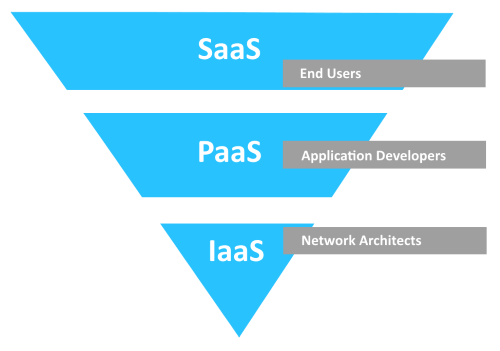
\includegraphics[width=1\textwidth]{imagenes/capitulo1/saas-paas-iaas.png}
    \caption{Clasificación de cloud computing en función del usuario.}
	\vspace{0.3cm}
    \label{clas-cloud-usuario}
\end{figure}

\begin{figure}
    \centering
    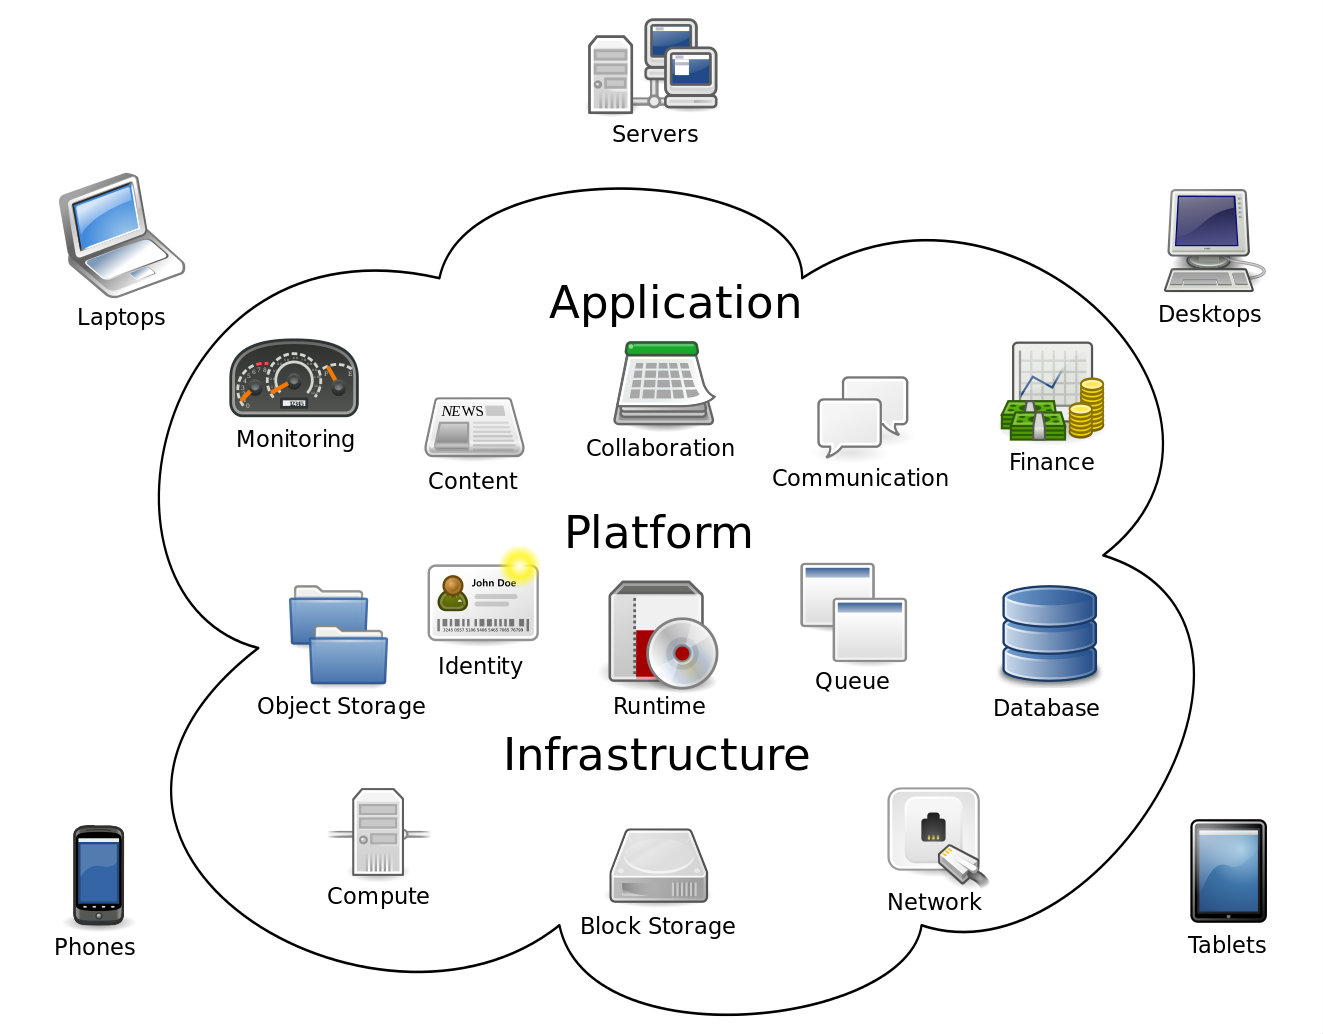
\includegraphics[width=1\textwidth]{imagenes/capitulo1/cloudcomputingDoit.png}
    \caption{Entorno Cloud Computing.}
	\vspace{0.3cm}
    \footnotesize{Fuente:Sam Johnston, "Cloud Computing", licensed underCC BY-SA 3.0 Unported, retrieved from Wikipedia)}
    \label{cloudcomputingDoit}
\end{figure}

En la Fig.\ref{cloudcomputingDoit} podemos ver representado todo lo que realmente podemos hacer en Cloud Computing. Vemos una nube a la que se puede acceder desde teléfonos, portátiles, servidores, escritorios y tabletas, realmente  es accesible desde  cualquier dispositivo. Dentro de la nube tenemos aplicaciones, plataformas e infraestructura. La infraestructura es la nube IaaS. En la nube IaaS, se están proporcionando recursos de cómputo, almacenamiento en bloque y redes. Luego está la plataforma, que es la plataforma como servicio en la nube (PaaS), en la que se proporcionan el almacenamiento de objetos, servicios de identificación, el tiempo de ejecución de los procesos, la cola y la base de datos. Y por último, en la capa más alta, tenemos la nube de aplicaciones que conocemos como nube de software como servicio (SaaS), en la que se están ofreciendo aplicaciones que pueden ser muy diversas, como los ejemplos que aparecen en la figura de monitorización, contenidos específicos, colaboración, comunicación o finanzas.

\subsection{Beneficios del cloud computing}
La computación en la nube presenta diversos beneficios. Hace que las IT sean flexibles para los usuarios así como también para los administradores:


\begin{itemize}
\item Proporciona fácil acceso a los activos de IT esenciales. Esto hace que sea lo más fácil posible para los usuarios emplear estos activos.
\end{itemize}

\begin{itemize}
\item Permite el autodespliegue. Los usuarios ya no necesitan un administrador de IT para implementar un nuevo servidor.
\end{itemize}

\begin{itemize}
\item Proporciona escalabilidad. Cuando se quede sin recursos físicos, es fácil agregar nuevos recursos.
\end{itemize}

\subsection{Modelo de Servicio IaaS}
Como hemos comentado ya, OpenStack se basa inicialmente en un modelo IaaS. Las nubes IaaS se pueden ofrecer de diferentes maneras, utilizando diferentes modelos de servicio:


\begin{itemize}
\item \textbf{Nube privada (\textit{Private Cloud})}. Una empresa crea una infraestructura IaaS que es solo para uso privado.
\end{itemize}

\begin{itemize}
\item \textbf{Nube pública (\textit{Public Cloud})}. La capacidad de la nube se ofrece como un servicio básico, como es el caso de la telefonía que ofrece un proveedor de telecomunicaciones. Los clientes contratan una parte de la infraestructura de la nube pública.
\end{itemize}

\begin{itemize}
\item \textbf{Nube híbrida (\textit{Hybrid Cloud})}. Este tipo de servicio IaaS es un modelo en el que una sesión en la nube consta de componentes de IaaS privados y públicos.
\end{itemize}

\subsection{Funcionamiento del modelo IaaS}
El funcionamiento de la computación IaaS es el siguiente: un usuario final accede al portal de la nube para derivar una máquina virtual. Mientras se prepara la instancia, el usuario final toma decisiones sobre redes, almacenamiento y seguridad. El almacenamiento persistente es opcional. Al final de la vida útil de la VM, esta desaparecerá. 

La nube IaaS proporciona una plataforma flexible para ejecutar contenedores, así como máquinas virtuales, de una manera flexible:

\begin{itemize}
\item La nube IaaS ofrece un portal de autoservicio.
\item También se proporciona almacenamiento escalable y conexión en red.
\end{itemize}

La computación en la nube IaaS funciona mejor para entornos que necesitan soluciones de IT flexibles. Si no necesitamos escalabilidad y autoservicio, quizás sea mejor optar por otro tipo de virtualización.

\section{NFV}

OpenStack Foundation describe NFV (\textit{Network Function Virtualization}) simplemente como una nueva forma de definir, crear y administrar funciones y servicios de red al reemplazar dispositivos físicos dedicados, con software que puede ser automatizado y administrado por OpenStack.

Al igual que las máquinas virtuales tomaron el lugar de muchos servidores dedicados en los centros de datos, NFV simplemente continúa con la mentalidad de reemplazar hardware físico inflexible y patentado por software. Una muestra de ello podemos verla en la Fig.\ref{clasicovsnfv}. 

Es aquí donde entran en juego las funciones de red virtuales (\textit{Virtual Network Function, VNF}). Las VNF son responsables de completar tareas de red específicas, y pueden ser máquinas virtuales, un contenedor, abarcar múltiples contenedores, múltiples máquinas virtuales o servidores bare metal, todo en la parte superior de la infraestructura informática y de red subyacente. 

Algunos ejemplos de VNF son puertas de enlace o \textit{gateways} móviles, \textit{routers}, servicios de red de entrega de contenido, cortafuegos, aceleradores WAN, DNS e incluso funciones básicas de paquete, todas ellas implementadas de manera virtual.


\begin{figure}[!ht]  \centering
    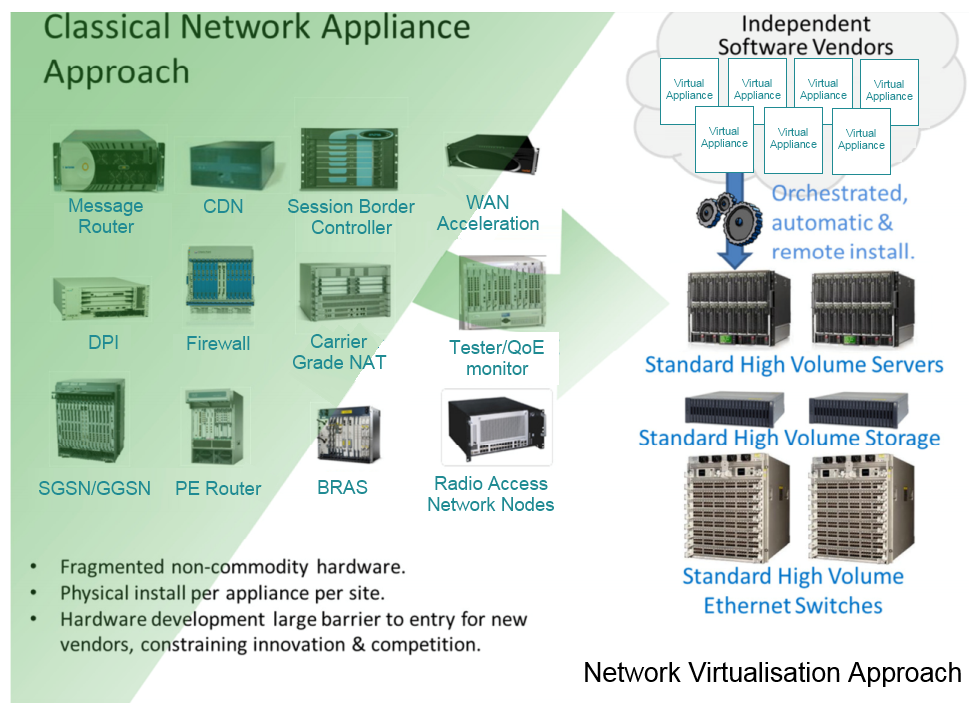
\includegraphics[width=1\textwidth]{imagenes/capitulo1/clasicovsnfv.png}
    \caption{Infraestructura física propietaria vs NFV.}
	\vspace{0.3cm}
    \footnotesize{Fuente: ETSI}
    \label{clasicovsnfv}
\end{figure}

\subsection{Beneficios de NFV}
En general, la mayoría de los beneficios de NFV se centran en agilidad, flexibilidad y simplicidad. Hoy en día, la industria de las telecomunicaciones es más competitiva que nunca y con los márgenes decrecientes, los costos y la demanda de nuevos servicios en aumento, NFV promete ofrecer algunas soluciones viables nuevas. Algunos de los beneficios detallados de NFV son los siguientes:


\begin{itemize}
\item Flexibilidad en la red a través del aprovisionamiento automatizado.
\item Aprovechamiento de la tecnología de código abierto y la innovación.
\item La flexibilidad de los controladores y complementos.
\item Completo acceso y uso de APIs que permiten un desarrollo más rápido.
\item El uso de hardware COTS (\textit{Commercial Off-The-Shelf}) frente a los dispositivos patentados.
\item Eficiencia operativa de una mejor orquestación en centros de datos, regiones y empresas.
\item Amplia gama disponible de documentación.
\end{itemize}

Los beneficios de NFV en OpenStack (frente a otras plataformas) aumentan la eficiencia y reducen los requisitos de Capex y Opex (inversión y gasto), potencia y espacio \cite{silverman_what_2018}.

\subsection{Diferencias entre NFV y SDN}
Aunque NFV y SDN son similares, ambas tienen claras diferencias. Tanto SDN como NFV son una forma de proporcionar funciones de red y automatización de redes heredadas, pero el objetivo de SDN es diferente de NFV. 

SDN consiste en la softwarización de las redes con el fin de simplificarlas, hacerlas más flexibles y reducir costes. Para ello usa un controlador encargado de ejecutar el software que gestiona elementos de red física como \textit{switches}, \textit{firewalls} y \textit{routers}, implementándose en la parte superior de la infraestructura de red física sobre la que se ejecuta la nube. 

NFV consume estas SDN como parte de una solución más grande y luego agrega funcionalidad adicional sobre las SDN. Algunos ejemplos de esto son \textit{firewalls} virtuales, filtros de contenido, aplicaciones antivirus, balanceadores de carga, \textit{routers}, etc. Estas funciones adicionales se denominan VNF o funciones de red virtuales. Aunque SDN juega un papel importante en el aprovisionamiento de recursos de NFV, la misión de NFV es virtualizar las funciones del nivel de aplicación sobre las de SDN \cite{silverman_difference_2018}.

A pesar de estas diferencias, en OpenStack se suele referenciar a los elementos de conectividad de red creados por \textit{Neutron}, proyecto que veremos en la sección \ref{subsec:Neutron}, como SDN.

\jorge{Yo quizá quitaría esa última frase. No aporta mucho sino que más bien lía. OpenStack usa una red SDN virtualizada (es decir, con switches software en lugar de switches físicos) para la red de interconexión de los nodos de cómputo y demás elementos. Pero eso no tiene nada que ver con que luego se implementen VNFs sobre OpenStack.}

\subsection{ETSI}
En los últimos años, la arquitectura NFV ha crecido más allá de ser simplemente una prueba de concepto para el administrador de infraestructura virtual (\textit{Virtual Infrastructure Manager}, VIM) principal que se utiliza para orquestar herramientas de gestión y orquestación de servicios automatizados para la infraestructura de NFV. Sin embargo, para definir mejor las especificaciones de lo que debería ser una plataforma de NFV, los grupos de expertos de OpenStack y los líderes de la industria de las telecomunicaciones han creado un gabinete específico alrededor de las NFV en Telecomunicaciones.

Fundada en 2012 por siete de los mayores operadores de redes de telecomunicaciones, la ETSI (European Telecommunication Standars Institute) creó el Grupo de especificación industrial de facto para NFV. Tras 5 años y más de 100 publicaciones después, lo que comenzó como una prueba de concepto ahora se ha convertido en la base para el estudio de mecanismos de de interoperabilidad. Los resultados de estas pruebas producen estándares para las organizaciones miembro y la industria europea de TIC en general.\cite{noauthor_etsi_nodate}

La ETSI actualmente está trabajando en la definición de la arquitectura y los requisitos para las VNF con el fin de:

\begin{itemize}
\item Maximizar la estabilidad y garantizar la confiabilidad del servicio.
\item Integración fluida con plataformas existentes y servicios heredados EMS, NMS, OSS, BSS y de orquestación de red.
\item Desarrollo de soluciones altamente efectivas y portátiles que tengan una amplia aplicación para proveedores de servicios.
\item Maximizar la eficiencia en la migración a nuevas plataformas virtualizadas.
\item Simplificar y optimizar las operaciones de telecomunicaciones.
\end{itemize}

\begin{figure}
    \centering
    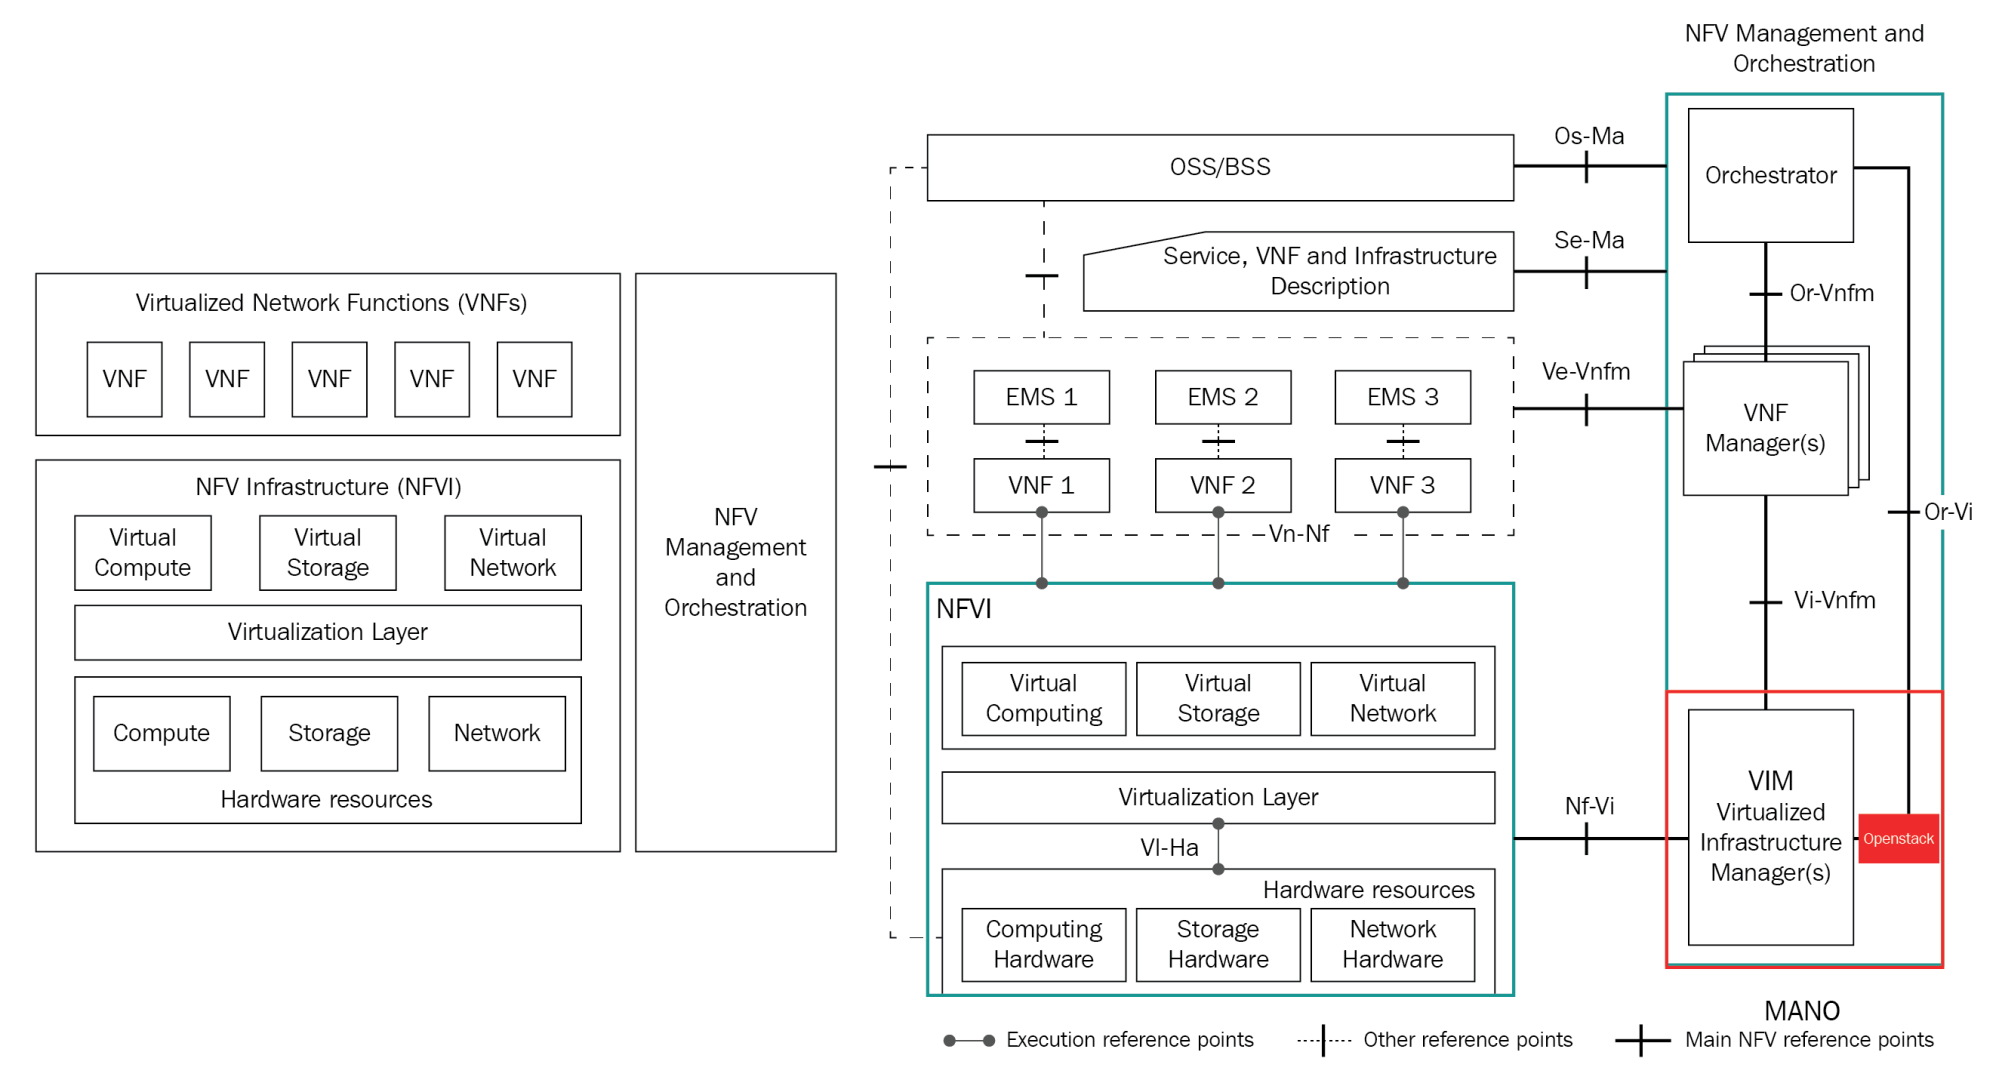
\includegraphics[width=1\textwidth]{imagenes/capitulo1/NFV_arquitectura.png}
    \caption{ETSI MANO Architectural Framework. Arquitectura para  NFV.}
	\vspace{0.3cm}
    \footnotesize{Fuente: ETSI NFV architecture}
    \label{arquitectura-NFV}
\end{figure}

\subsection{El rol de Openstack en NFV}
En la imagen de la Fig.\ref{arquitectura-NFV} podemos ver la base para construir todos los sistemas NFV. En la parte de la izquierda se muestra la arquitectura general de NFV y los principales componentes mientras que en la derecha tenemos como esos componentes funcionan conjuntamente.

El rol de OpenStack es del VIM. El VIM orquesta el hardware contenido en el cuadro de infraestructura NFVI (NFV Infrastructure) para ejecutar las VNFs.



\chapter{Estado del arte} 
\label{chap:estadodelarte}

A pesar de ser la elección de OpenStack un requisito del proyecto, los motivos de su elección frente al resto de plataformas libres y de pago son varios. 

En este capítulo vamos a proceder a describir los servicios y características \textit{cloud} que ofrecen algunos de los proveedores de servicio IaaS principales y justificaremos la elección de OpenStack haciendo una pequeña comparativa.

También veremos algunas de las empresas más fuertes que ofrecen un servicio de computación en la nube basado en OpenStack para a continuación justificar la vía por la que optaremos.

Para finalizar el capítulo veremos algunos datos que nos darán una clara imagen de la importancia de OpenStack en los despliegues de IT y el panorama TIC actual.

\section{Plataformas de Cloud Computing}
Al desplegar un proyecto de IaaS pretendiendo crear nuestra propia nube, inmediatamente se nos vienen a la cabeza proveedores de servicio de pago como Amazon Web Services, Rackspace Cloud Server, Mirantis, Microsoft Windows Azure, VMware o Google Cloud. 

Existen otros proveedores que ofrecen plataformas open source como es el caso de Eucalyptus, OpenNebula o CloudStack.

Sin mas dilación, vamos a ver las características principales de algunos de estos proveedores (dos de pago y dos open source) los cuales hemos elegido por su relevancia dentro de los servicios \textit{cloud}.

\subsection{Amazon Web Services}

\begin{figure}
    \centering
    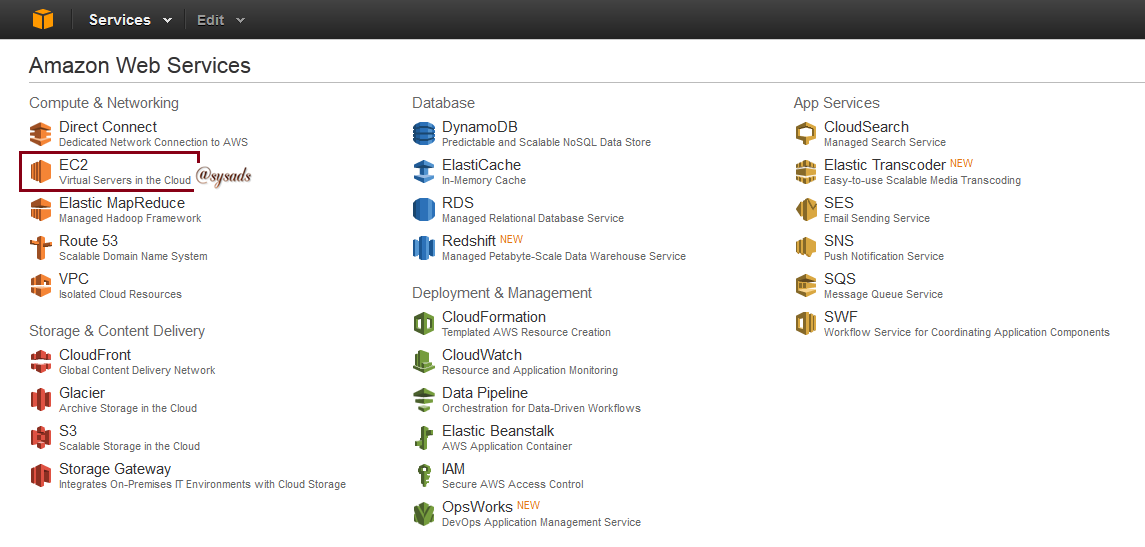
\includegraphics[width=0.7\textwidth]{imagenes/capitulo2/amazon.png}
    \caption{Panel de control de Amazon Web Services.}
	\vspace{0.3cm}
    \footnotesize{Fuente: Amazon}
    \label{amazon}
\end{figure}

Amazon Elastic Compute Cloud (Amazon EC2) es un servicio web que proporciona capacidad informática con tamaño modificable en la nube. Está diseñado para facilitar a los desarrolladores recursos informáticos escalables vía web a través de una sencilla interfaz cuyo panel de control podemos ver en la Fig.\ref{amazon}. Según la propia empresa ofrecen \cite{noauthor_aws_nodate}:

\begin{itemize}
\item Reducción del tiempo necesario para obtener y arrancar nuevas instancias de un servidor en minutos, lo que permite escalar rápidamente la capacidad, ya sea aumentándola o reduciéndola, según cambien sus necesidades.
\item Modelo económico consecuente. Pago sólo por la capacidad que se utiliza realmente.
\item Amazon EC2 proporciona a los desarrolladores las herramientas necesarias para crear aplicaciones resistentes a errores y para aislarse de los casos de error más comunes.
\item Compatibilidad con otros servicios de AWS.
\item Fiabilidad. El servicio se ejecuta en los centros de datos e infraestructura de red acreditados de Amazon.
\item Seguridad. Mecanismos de VPC, listas de acceso, VPN IPsec e instancias aisladas.
\item Asequibilidad. Amazon EC2 ofrece ventajas financieras dentro su corporación.
\end{itemize}

\subsection{VMware}
VMware es una compañía suministradora de servicios de virtualización por software donde las máquinas virtuales proporcionan un ambiente de ejecución similar, a todos los efectos, a un computador físico. Entre sus servicios de virtualización ofrece \cite{noauthor_virtualizacion_nodate}:

\begin{itemize}
\item Virtualización de servidores.
\item Virtualización de redes.
\item Virtualización de escritorios.
\item Virtualización de aplicaciones.
\item Virtualización de almacenamiento.
\end{itemize}

\subsection{VMware vSphere}
Dentro de las opciones que nos brinda VMware cabe destacar VMware vSphere, diseñado para organizaciones que desean optimizar los activos de infraestructura
tecnológica existentes y demorar las costosas expansiones del centro de datos,
\textit{VMware® vSphere® Standard Edition} proporciona una solución de consolidación básica de las aplicaciones, a fin de reducir drásticamente los costes de hardware, además de acelerar la implementación de las aplicaciones sin tener que programar ningún tiempo de inactividad.

VMware vSphere permite a los usuarios ejecutar aplicaciones críticas para el negocio con confianza y responder con mayor rapidez a las necesidades empresariales acelerando el cambio hacia la computación en la nube para los centros de datos.

Esta herramienta ofrece una serie de servicios \cite{noauthor_vmware-vsphere-datasheet.pdf_nodate} como vemos en la Fig.\ref{VMware} que la dotan de ventajas entre las que destacamos:

\begin{itemize}
\item Mayor eficiencia gracias a la automatización y mejora del rendimiento del hardware pasando del 15 al 80\% de utilización.
\item Disminución de gastos de propiedad y operativos.
\item Escalabilidad y disponibilidad.
\item Plataforma basada en estándares.
\end{itemize}

\begin{figure}
    \centering
    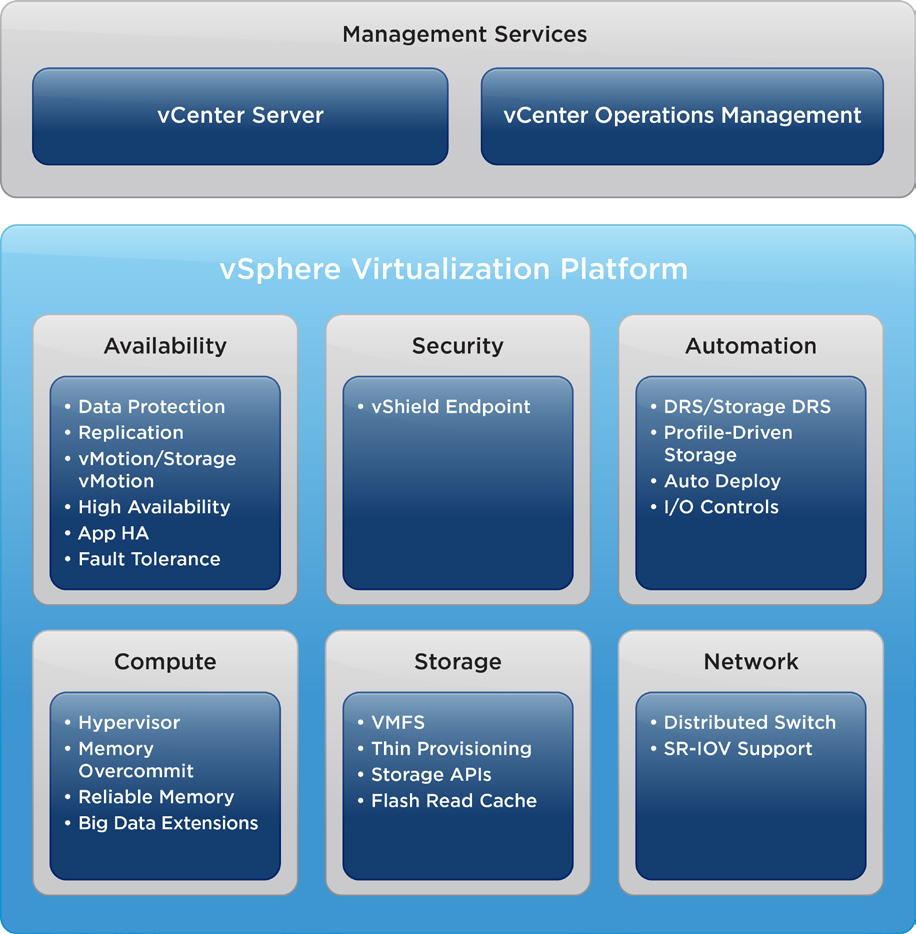
\includegraphics[width=0.7\textwidth]{imagenes/capitulo2/VMware.png}
    \caption{Servicios de VMware vSphere.}
	\vspace{0.3cm}
    \footnotesize{Fuente: VMware}
    \label{VMware}
\end{figure}

\subsection{Apache CloudStack}
Apache CloudStack es un proyecto de alto nivel de la Fundación de Software
Apache. El proyecto desarrolla software de código abierto y nubes con infraestructura
como servicio (IaaS).
Este proyecto provee las herramientas necesarias para entregar nubes públicas de
manera fiable y escalable.
Entre sus características se encuentran las siguientes \cite{noauthor_apache_nodate}:

\begin{itemize}
\item Trabaja con hipervisores como Xen, KVM, HyperfV o Vmware ESXiconVsphere.
\item Provee una interfaz sencilla para el manejo de toda la operativa de un
IaaS por medio de  una interfaz visual o de comandos.
\item Tiene una API Nativa.
\item Compatibilidad con Amazon S3 y EC2.
\item Maneja almacenamiento para instancias basado en los hipervisores
además de plantillas, capturas de instancias e Imágenes ISO como
almacenamiento secundario.
\item Servicios de redes desde la capa de enlace a la de aplicación como por ejemplo: DHCP, NAT, cortafuegos y VPNs.
\item Está separada en partes: Red, cómputo y almacenamiento.
\item Soporte multi-usario o multi-tenant: a un proyecto pueden acceder varios usuarios concurrentemente.
\end{itemize}

\subsection{OpenNebula}
OpenNebula surge como un proyecto de investigación llevado a cabo desde la Universidad Complutense de Madrid. Esta enfocado en la computación distribuida, virtualización y plataformas IaaS bajo una licencia Apache 2.0.\cite{noauthor_about_nodate}

Esta plataforma esta dotada con algunas funcionalidades que convierten a OpenNebula en un gestor de VDC (Virtual Data Center) con el que encargarse desde la capa más básica de red y almacenamiento, hasta los procesos de gestión de usuarios, tiempos de uso, explotación de recursos y escalabilidad:

\begin{itemize}
\item Gestión de recursos flexible y despliegue de máquinas pre-configuradas.
\item Gestión de usuarios: uso, facturación, provisionamiento.
\item Gestión de perfiles de seguridad.
\item Gestión de redes.
\item Gestión de almacenamiento.
\item Mecanismos de alta disponibilidad y clusters.
\item Creación de virtual centers, zonas o nubes híbridas.
\item Aplicaciones en Market App.
\item Servicios de monitorización. 
\item API para integración.
\item Sistema de Hooks.
\item Compatible con hipervisores Xen, KVM, QUEMU, VMWare ESXI, ESX Server.
\end{itemize}

\subsection{Comparativa de las plataformas Cloud de pago con OpenStack}

El principal motivo de la elección de OpenStack frente a otras plataformas de pago como VMware o AWS, es precisamente el económico. La filosofía del proyecto es que se realice mediante una plataforma cloud de software libre apta para la investigación. 

Además OpenStack cuenta con todos los servicios que estas plataformas de pago ofrecen. La principal diferencia radica en el hecho de que las plataformas de pagos ofrecen sus propia infraestructura y el despliegue y uso es mucho más sencillo e intuitivo. Basta con contratar aquellos servicios que queramos y estos serán administrados por nosotros.

Esto no es obviamente algo que deseemos pues el objetivo de nuestro proyecto es realizar el despliegue de nuestra propia infraestructura y adaptarla a aquellos recursos y servicios que queramos y de los que podamos disponer.

\subsection{Comparativa de las plataformas Cloud open source con OpenStack}

Eucalyptus, OpenNebula y CloudStack, son los principales competidores a la hora de realizar nuestra elección frente a OpenStack. 

El primer caso, Eucalyptus, si ni quiera existe ya hoy en día, razón por la cuál no hemos hablado de dicho proyecto.

Con respecto a OpenNebula y CloudStack, una característica fundamental para tomar la decisión se representa en la Fig.\ref{comparativa cloud open source} extraída de la web de OpenNebula \cite{noauthor_eucalyptus_nodate} donde podemos ver una comparativa de las distintas herramientas en función de dos criterios:

\begin{itemize}
\item El modelo de cloud:
\begin{itemize}
\item Virtualización del centro de datos. Entender la nube como una extensión de la virtualización en el centro de datos.
\item Provisión de infraestructura: Herramienta de aprovisionamiento para suministrar recursos virtualizados según demanda.
\end{itemize}
\item La flexibilidad.
\end{itemize}

\begin{figure}
    \centering
    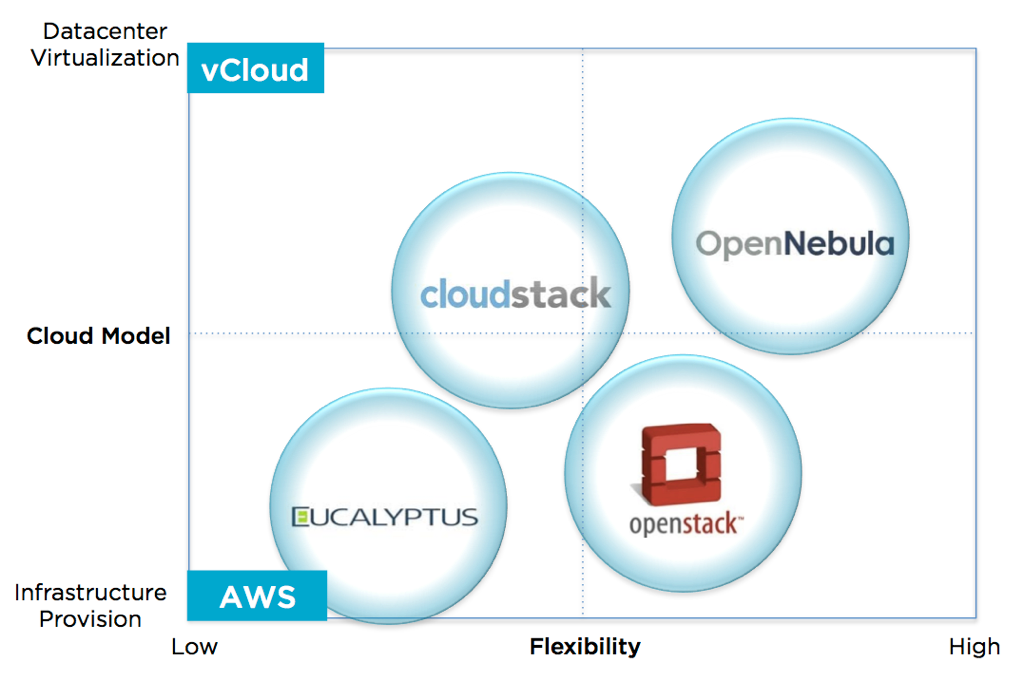
\includegraphics[width=0.7\textwidth]{imagenes/capitulo2/comparativaCloudPublica.png}
    \caption{Comparativa entre clouds open source en función del uso y la flexibilidad.}
	\vspace{0.3cm}
    \footnotesize{Fuente: Ignacio M.Llorente, “Eucalyptus, CloudStack, OpenStack and OpenNebula: A Tale of Two Cloud Models", OpenNebula, 2013}
    \label{comparativa cloud open source}
\end{figure}

Cómo vemos, OpenStack se postula como la plataforma más flexible para construir nuestra IaaS. Además, posee todas las características de sus competidores incorporando una actualización constante de los proyectos que forman parte de esta herramienta y que podemos incorporar a nuestro proyecto de forma modular en función de nuestras necesidades.

Para acabar la comparación, un estudio realizado en 2013 por Qingye Jiang \cite{qingye_jiang_cy12-q4_2013} en el que hace una comparativa de estas cuatro plataformas, ya mostraba la clara tendencia de comunidad, empresas y desarrolladores a usar OpenStack. En la Fig.\ref{comparativa del chino} vemos una extracción del estudio en el que se aprecia el número de participantes mensual en los proyectos y como OpenStack irrumpió desde un inicio tomando clara ventaja al resto de soluciones.

\begin{figure}
    \centering
    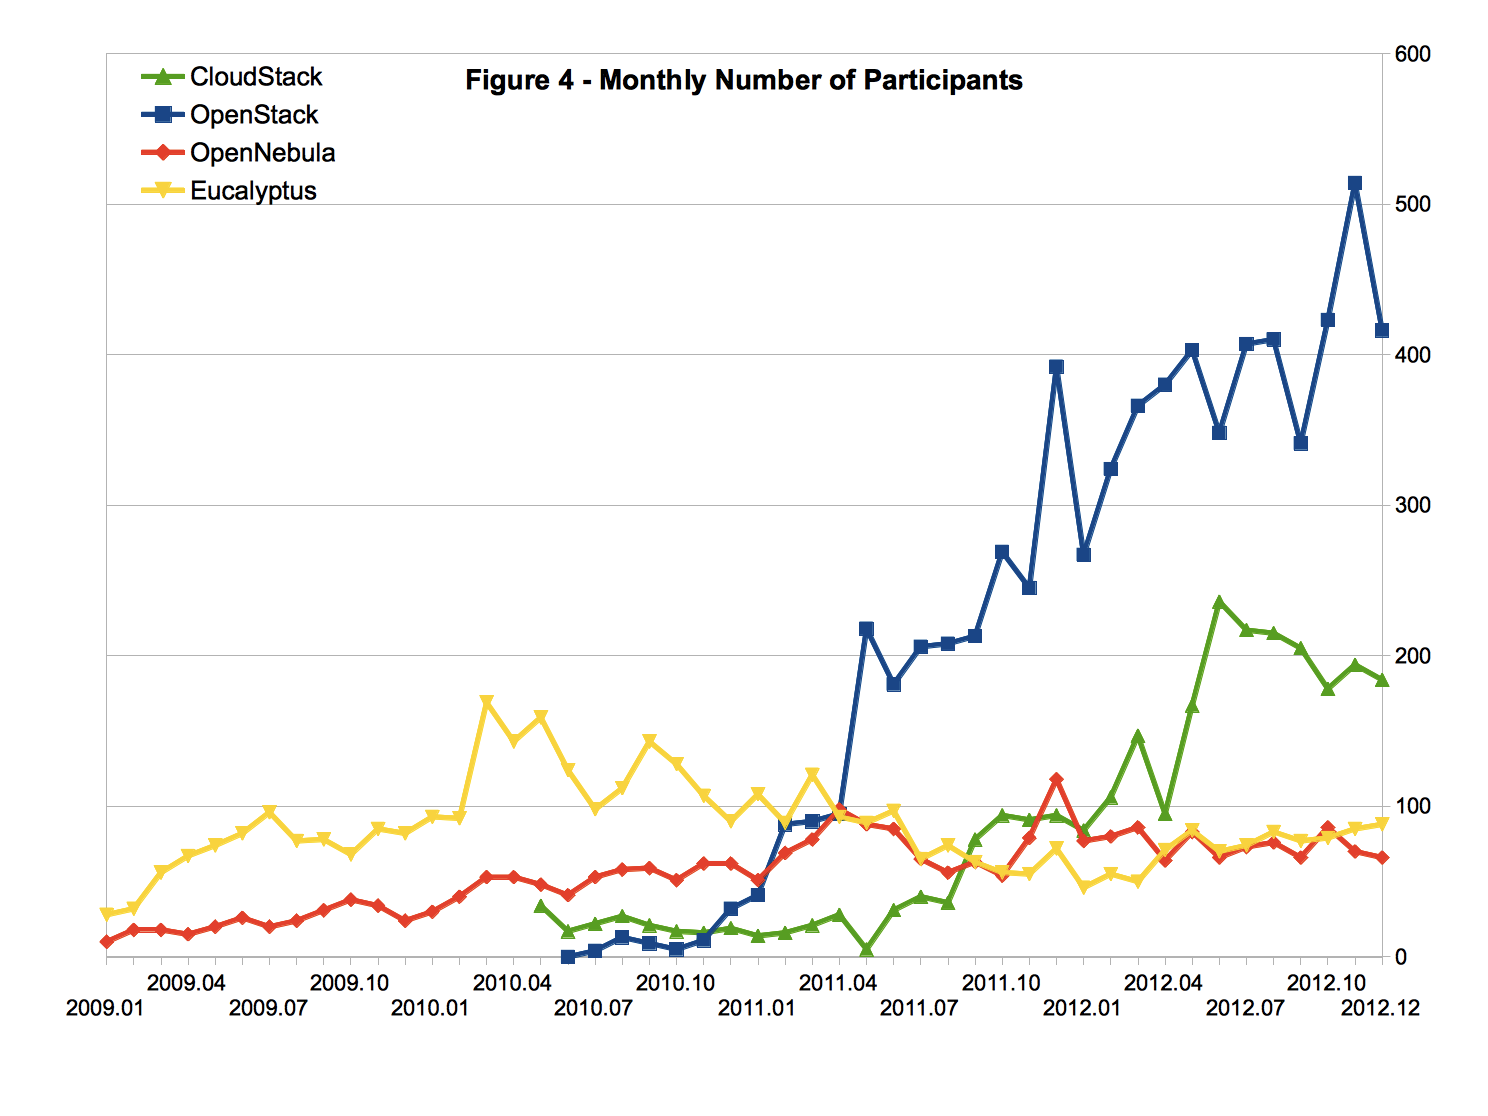
\includegraphics[width=0.7\textwidth]{imagenes/capitulo2/mesOpenStack.png}
    \caption{Número de participantes mensual.}
	\vspace{0.3cm}
    \footnotesize{Fuente: Qingye Jiang, “OpenStack vs OpenNebula vs Eucalyptus vs CloudStack", Open Source IaaS Community Analysis, 2013}
    \label{comparativa del chino}
\end{figure}


\section{Vendedores de OpenStack}
Son varios los proveedores que ofrecen sus productos y servicios junto con OpenStack. Estos proveedores abarcan desde distribuidores de hipervisores con estrecha integración a su plataforma hasta proveedores en la nube que ofrecen versiones de cloud públicas, privadas o híbridas. En lo que sigue de la sección, nombraremos algunas de las más representativas del mercado \cite{shrivastwa_vendor_2016}.

\subsection{VMware Integrated OpenStack}

De esta solución podemos destacar:

\begin{itemize}
\item VMware Integrated OpenStack viene con un proveedor de hipervisores. 
\item Se  puede obtener de forma gratuita con una licencia enterprise plus de VMware.
\item Se integra muy bien en el cliente web vSphere y despliega un OpenStack enfocado a un entorno productivo en solo unos pocos clics.
\item Está estrechamente integrado con el ESXi Hypervisor. 
\item La última versión integrada es \textit{Kilo}.
\end{itemize}


Su popularidad radica en el hecho de que existen muchas empresas que ya han hecho una inversión considerable en términos de licencias de VMware para hipervisores \cite{noauthor_integrated_nodate}.

\subsection{Rackspace Cloud}
Rackspace necesita una mención especial, no solo porque ejecutan una famosa nube pública basada en OpenStack, sino también porque si no fuera por ellos, ni siquiera tendríamos OpenStack ya que fueron Rackspace y NASA los que comenzaron este proyecto en 2010. Sin embargo, todavía están en la versión \textit{Icehouse} con el hipervisor Xen \cite{noauthor_choosing_nodate}.

\subsection{HP Helion}
En el segmento de software libre y  código abierto (FOSS) para productos en la nube, OpenStack y Eucalyptus fueron dos productos que resolvieron los mismos problemas. HP adquirió Eucalyptus y lo ha agregó a sus ofertas en la nube de Helion. Actualmente incorpora también OpenStack pudiendo elegir entre ambas opciones \cite{noauthor_software_nodate}.

\subsection{Cisco OpenStack}
Cisco tiene una distribución OpenStack que se ejecuta en su chasis y proporciona soluciones en la nube, en su mayoría privadas, para las empresas que permiten una fácil implementación de una instalación compatible con OpenStack en sus centros de datos \cite{noauthor_cisco_nodate}.

\subsection{Mirantis OpenStack}
Mirantis OpenStack es uno de los más flexibles y al mismo tiempo, una distribución abierta de OpenStack que además ofrece servicio de soporte técnico.

En cuanto a los hipervisores, se abarca desde Xen, Docker, Hyper-V, ESXi, LXC (contenedores Linux), QEMU y KVM. Por lo tanto, si se desean opciones más respaldadas en términos de hipervisores, esta será la elección ideal \cite{noauthor_mirantis_nodate}.

\subsection{SwiftStack}
SwiftStack es un ejemplo de implementación parcial de OpenStack. Solo implementa como su nombre lo indica, Swift, el servicio de almacenamiento de objetos de OpenStack \cite{noauthor_swiftstack_nodate}.

\subsection{IBM Cloud Manager}
El administrador de IBM Cloud pertenece al gigante tecnológico IBM, que proporciona integración con el hipervisor z/VM ejecutándose en mainframes. También proporciona conjuntos de herramientas de gestión junto con su distribución. Su lanzamiento actual se basa en \textit{Juno} \cite{peterson2700042wjc_ibm_2009}.

\subsection{Suse Cloud}
Basada en OpenStack y Crowbar, esta oferta de nube privada admite implementaciones mixtas de hipervisor en la nube basadas en la versión de OpenStack de \textit{Icehouse} \cite{noauthor_suse_nodate}.

\subsection{Sobre los vendedores}
De nuevo, a la hora de implementar nuestra IaaS, no vamos a optar por ninguno de los vendedores citados sino que, partiendo de la instalación de Ubuntu Server en nuestros servidores, realizaremos nuestro propio despliegue por varios motivos:

\begin{itemize}
\item El primero vuelve a ser el económico. Como proyecto de investigación y prueba de concepto que estamos realizando, la barrera económico es clave en el desarrollo del proyecto.
\item Todas las soluciones citadas dan soporte sólo a algunos de los proyectos que forman OpenStack. De este modo, proyectos menos conocidos o usados por su naturaleza, como el caso de Tacker, no tendrían cabida. Además, así podremos incorporar sólo aquellos proyectos que nos ayuden a cumplir nuestros objetivos.
\item Otro motivo es la naturaleza académica del proyecto. Realizando nuestro propio despliegue alcanzaremos un conocimiento mucho más profundo acerca de los aspectos relativos al despliegue de una nube IaaS.
\item Por último, la mayoría de distribuidores se basan en versiones de OpenStack que ya no tiene soporte. En nuestro caso elegiremos para el desarrollo Queens, que es la última versión estable \cite{noauthor_releases:_nodate} del proyecto e incorpora actualizaciones de todos los servicios y proyectos de OpenStack. 
\end{itemize}



\section{El papel de OpenStack en el ámbito IT}

El proyecto OpenStack surge de la colaboración global de desarrolladores tecnológicos y de computación en la nube que crearon esta plataforma. Cientos de las marcas más grandes del mundo incluyendo AT\&T, Bloomberg, Best Buy, Comcast, eBay, PayPal, SAP, Time Warner Cable, Verizon, Visa, Walmart, Wells Fargo y Yahoo, por nombrar algunos, confían en OpenStack para el funcionamiento diario de sus negocio, reduciendo costos y ganando en movilidad. 

\begin{figure}
    \centering
    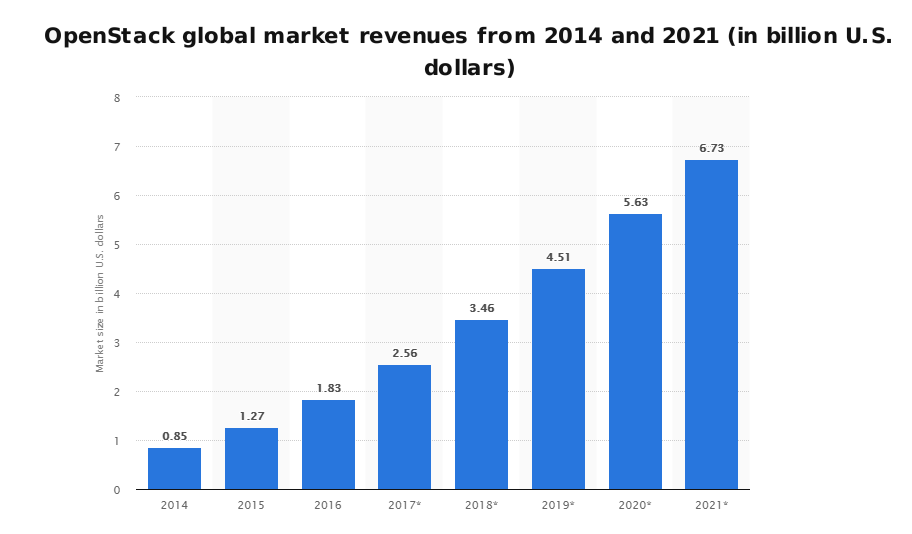
\includegraphics[width=0.7\textwidth]{imagenes/capitulo2/ganancias_OpenStack.png}
    \caption{Ingresos globales de mercado de OpenStack de 2014 a 2021 en miles de millones de dólares estadounidenses
.}
	\vspace{0.3cm}
    \footnotesize{Fuente: Statista}
    \label{ganancias_OpenStack}
\end{figure}

OpenStack es utilizado por el 50\% de la lista de las compañías que más ingresos generan en EE.UU. conocida como \textit{US Fortune 100} \cite{noauthor_fortune_nodate}, que abarca industrias que incluyen todo tipo de servicios, finanzas, fabricación, medios de comunicación, investigación, gubernamental, universitarios, venta minorista, tecnología y telecomunicaciones. Para mostrar este hecho en términos económicos, en la Fig.\ref{ganancias_OpenStack} se muestra un estudio del portal de estadísticas \textit{Statista} \cite{noauthor_statistic_nodate} donde se estima que las ganancias que generará la plataforma solo este año serán de aproximadamente 3.46 billones de dólares americanos con una tendencia anual creciente.


OpenStack está basado en estándares abiertos.  Uno de los principales elementos de OpenStack es la API abierta (\textit{Application Program Interface}), que es un conjunto de definiciones de rutina, protocolos y herramientas para crear software y aplicaciones. Debido a que la API OpenStack está tan bien desarrollada, atrae a los desarrolladores, facilitando su trabajo.


Lanzado en 2010, el proyecto OpenStack, cuenta con una de las comunidades de código abierto de más rápido crecimiento en el mundo, está respaldado por una comunidad vibrante de desarrolladores y algunos de los nombres más grandes en la industria. Hasta la fecha, posee una contribución de más de 20 millones de líneas de código por más de 90000 personas y 600 empresas en 185 países. En la Fig.\ref{Alcance de OpenStack} podemos ver un resumen de las dimensiones del proyecto hasta la fecha.

\begin{figure}
    \centering
    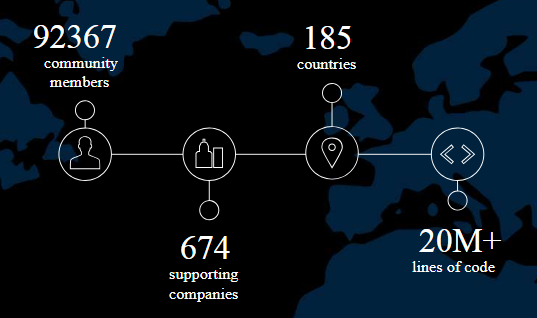
\includegraphics[width=0.7\textwidth]{imagenes/capitulo2/community.png}
    \caption{Alcance de OpenStack.}
	\vspace{0.3cm}
    \label{Alcance de OpenStack}
\end{figure}

Por tanto, el hecho de ser una plataforma open source unido a que es la herramienta más usada para entornos cloud en la actualidad y la que cuenta con la mayor comunidad en su ámbito y un número enorme de empresas contribuidoras fundamentales en cualquier desarrollo tecnológico de hoy día, hace que la elección sea sencilla.

\subsection{Casos de éxito}

OpenStack es el producto de nube más exitoso, las implementaciones con él son demasiadas para detallarlas. En esta sección, veremos algunos de los casos de uso más comunes donde se puede ver OpenStack en acción.\cite{shrivastwa_openstack_2015}

\begin{itemize}
\item \textbf{Enterprise Private Cloud}. Uno de los casos de uso más comunes si nos encontramos en la organización de IT de cualquier empresa que opte por ofrecer una nube privada a sus diferentes unidades de negocios, que ahora demandan agilidad, flexibilidad y menor tiempo de lanzamiento al mercado, es sin duda OpenStack.

Algunas de las empresas que lo han adoptado son eBay, Alcatel-Lucent, BMW, PayPal, NASA y Sony, entre otras.

\item \textbf{Proveedores de servicio}. Si miramos líneas de negocio de proveedores de servicios, como un proveedor de centro de datos, es posible que este desee comenzar a ofrecer servicios en la nube. La naturaleza distribuida de OpenStack puede ayudarlo a crear una nube con el fin de proveer del servicio de un centro de datos virtualizado a sus usuarios, agregando algunas integraciones adicionales por encima de la oferta estándar de OpenStack, como conjuntos de herramientas y SLA.

Hay varios proveedores de servicios que usan OpenStack hoy como AT \& T, Telstra, CCS (Cisco Cloud Services), Korea Telecom, Dream Host, y más.

\item\textbf{Escuelas / Centros de investigación}. Incluso las escuelas usan OpenStack en sus laboratorios para proporcionar rápidamente diferentes tipos de cargas de trabajo para los estudiantes, el personal y los profesores de investigación que están llevando a cabo proyectos o investigando en varios campos de su estudio. No depender del equipo de IT reduce en gran medida el tiempo requerido para comenzar un proyecto.

Algunos de los ejemplos notables son CERN, MIT, CSAIL, etc.

\item \textbf{Proveedores web, SaaS}. Este tipo de empresas necesitan agilidad. Hay varios cientos de ellos y sus criterios de éxito dependen de cuán rápido puedan incorporar nuevas características a sus productos, por lo tanto, el Dev / Test y todo el paradigma DevOps para ellos se convierte en la clave para la supervivencia y OpenStack puede ayudarlos a lograrlo. Estas compañías inevitablemente usan OpenStack o un equivalente para abordar esta tarea.

Algunos ejemplos en este segmento serían MercadoLibre.com o Platform 9.
\end{itemize}


\chapter{Planificación y costes} \label{chap:planificacionycostes}
El primer paso, una vez que hemos esbozado la idea del proyecto que tenemos entre manos, consiste en realizar una planificación detallada en la que establezcamos y definamos de manera precisa las tareas necesarias para abordarlo teniendo en cuenta todos los aspectos que pueden influir en el correcto desarrollo del mismo.

Para lograr la implantación de nuestra cloud y dar así un servicio de IaaS, tenemos que pasar por diversas fases de desarrollo que comentaremos en el siguiente punto. Además, se necesita de una planificación temporal que acompañe a las tareas y que veremos también en este capítulo.

No podemos olvidar los recursos necesarios para la elaboración del proyecto tanto humanos, como hardware,  software y servicios. Estos recursos se han escogido, en ocasiones, basándonos en el uso de los mismos durante la realización de los estudios de Grado.

Finalmente concluiremos este punto con un desglose del coste estimado de los distintos elementos del proyecto de los que iremos hablando a lo largo del capítulo y que darán un coste final total como colofón.


\section{Fases de desarrollo}
En esta sección vamos a listar todas las tareas que se van a llevar a cabo, agrupándolas en distintas fases y acompañándolas de una pequeña descripción. 

Las distintas fases de desarrollo junto las tareas de las que se componen, así como las fechas de inicio y fin y el número de días empleado para cada una se muestran en la Fig.\ref{fig:tareas}. Como se puede apreciar existe una clara relación entre las tareas y la estructura de la memoria \ref{subchap:estrucutramemoria}. Además tenemos los correspondientes diagramas de Gantt que muestran la contemporización de tareas por meses, en la Fig.\ref{fig:ganttMes} y para una mejor visualización por trimestres en la Fig.\ref{fig:gantTrimes}. 

En estas figuras podemos ver que la duración estimada del proyecto en días laborales desde que se inicia la primera tarea hasta que finaliza la última, entre las cuales está planificada la realizarán algunas tareas en paralelo, hacen un total de 223 días, de los cuales se estima un trabajo de de 3 horas diarias en días laborales, lo cuál tendremos en cuenta en el apartado \ref{subchap:costeshumanos} de costes humanos .

\begin{figure}
    \centering
    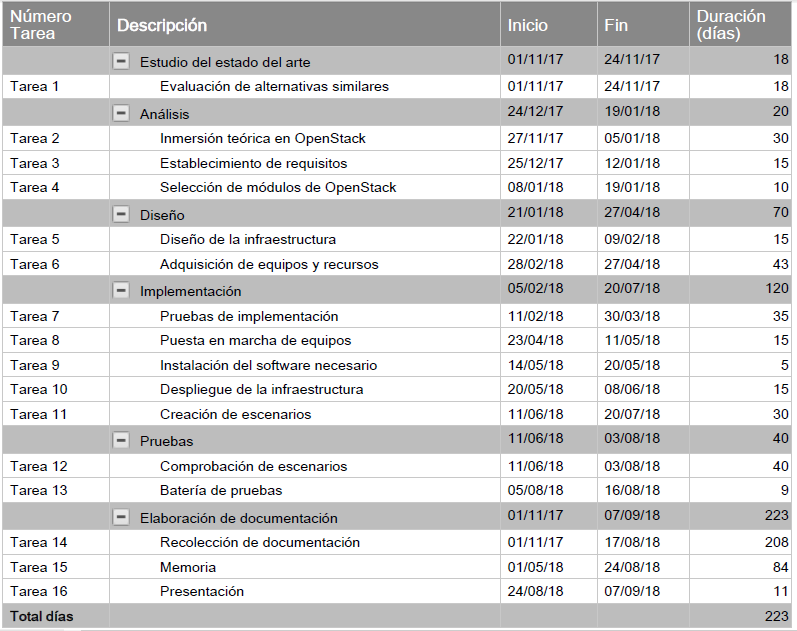
\includegraphics[width=1\textwidth]{imagenes/capitulo3/tareas.png}
    \caption{Planificación de tareas.}
	\vspace{0.3cm}
    \label{fig:tareas}
\end{figure}

\begin{figure}
    \centering
    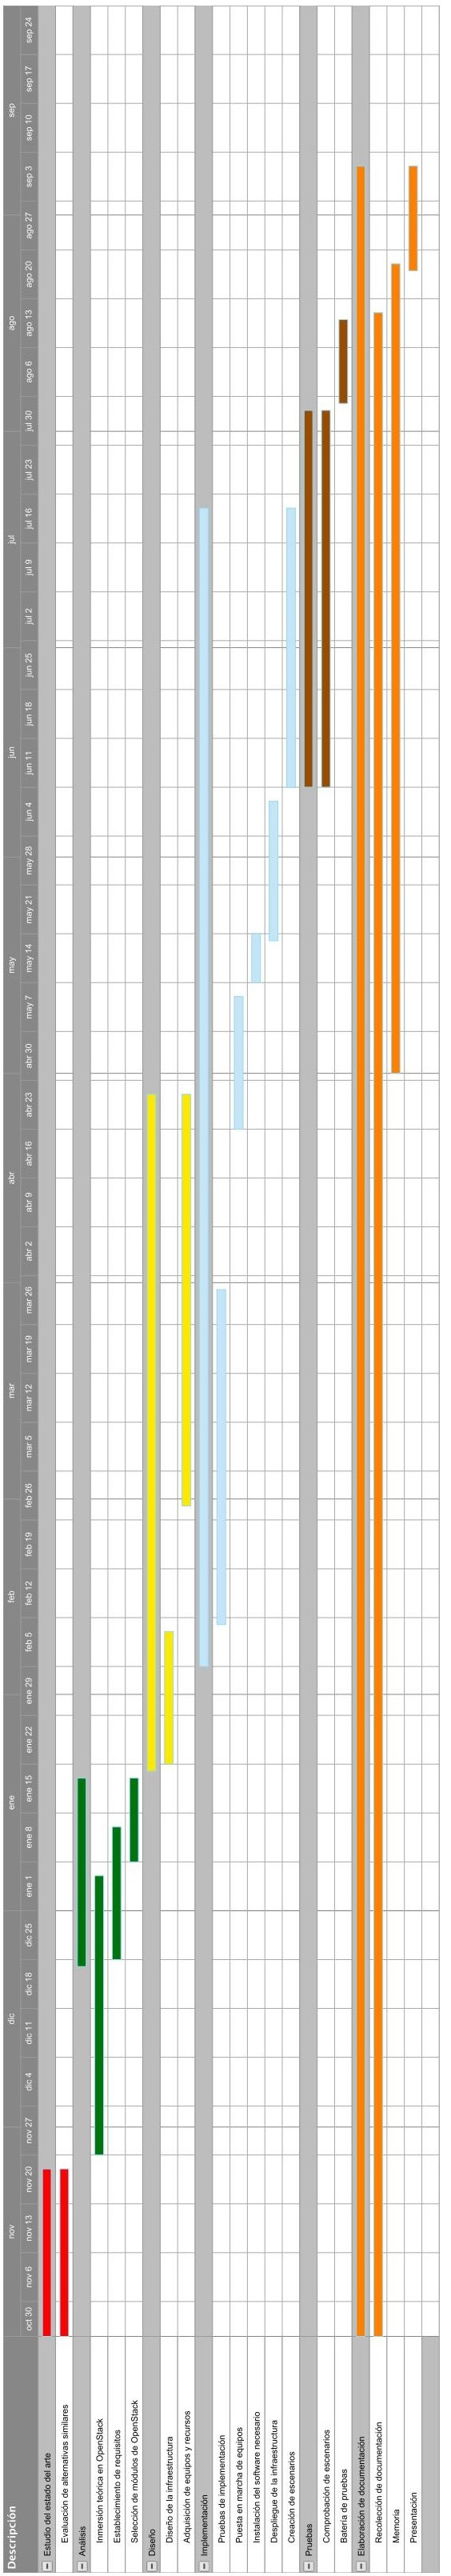
\includegraphics[width=0.32\textwidth]{imagenes/capitulo3/0001.jpg}
    \caption{Diagrama de Gantt mensual.}
	\vspace{0.3cm}
    \label{fig:ganttMes}
\end{figure}


\begin{figure}
    \centering
    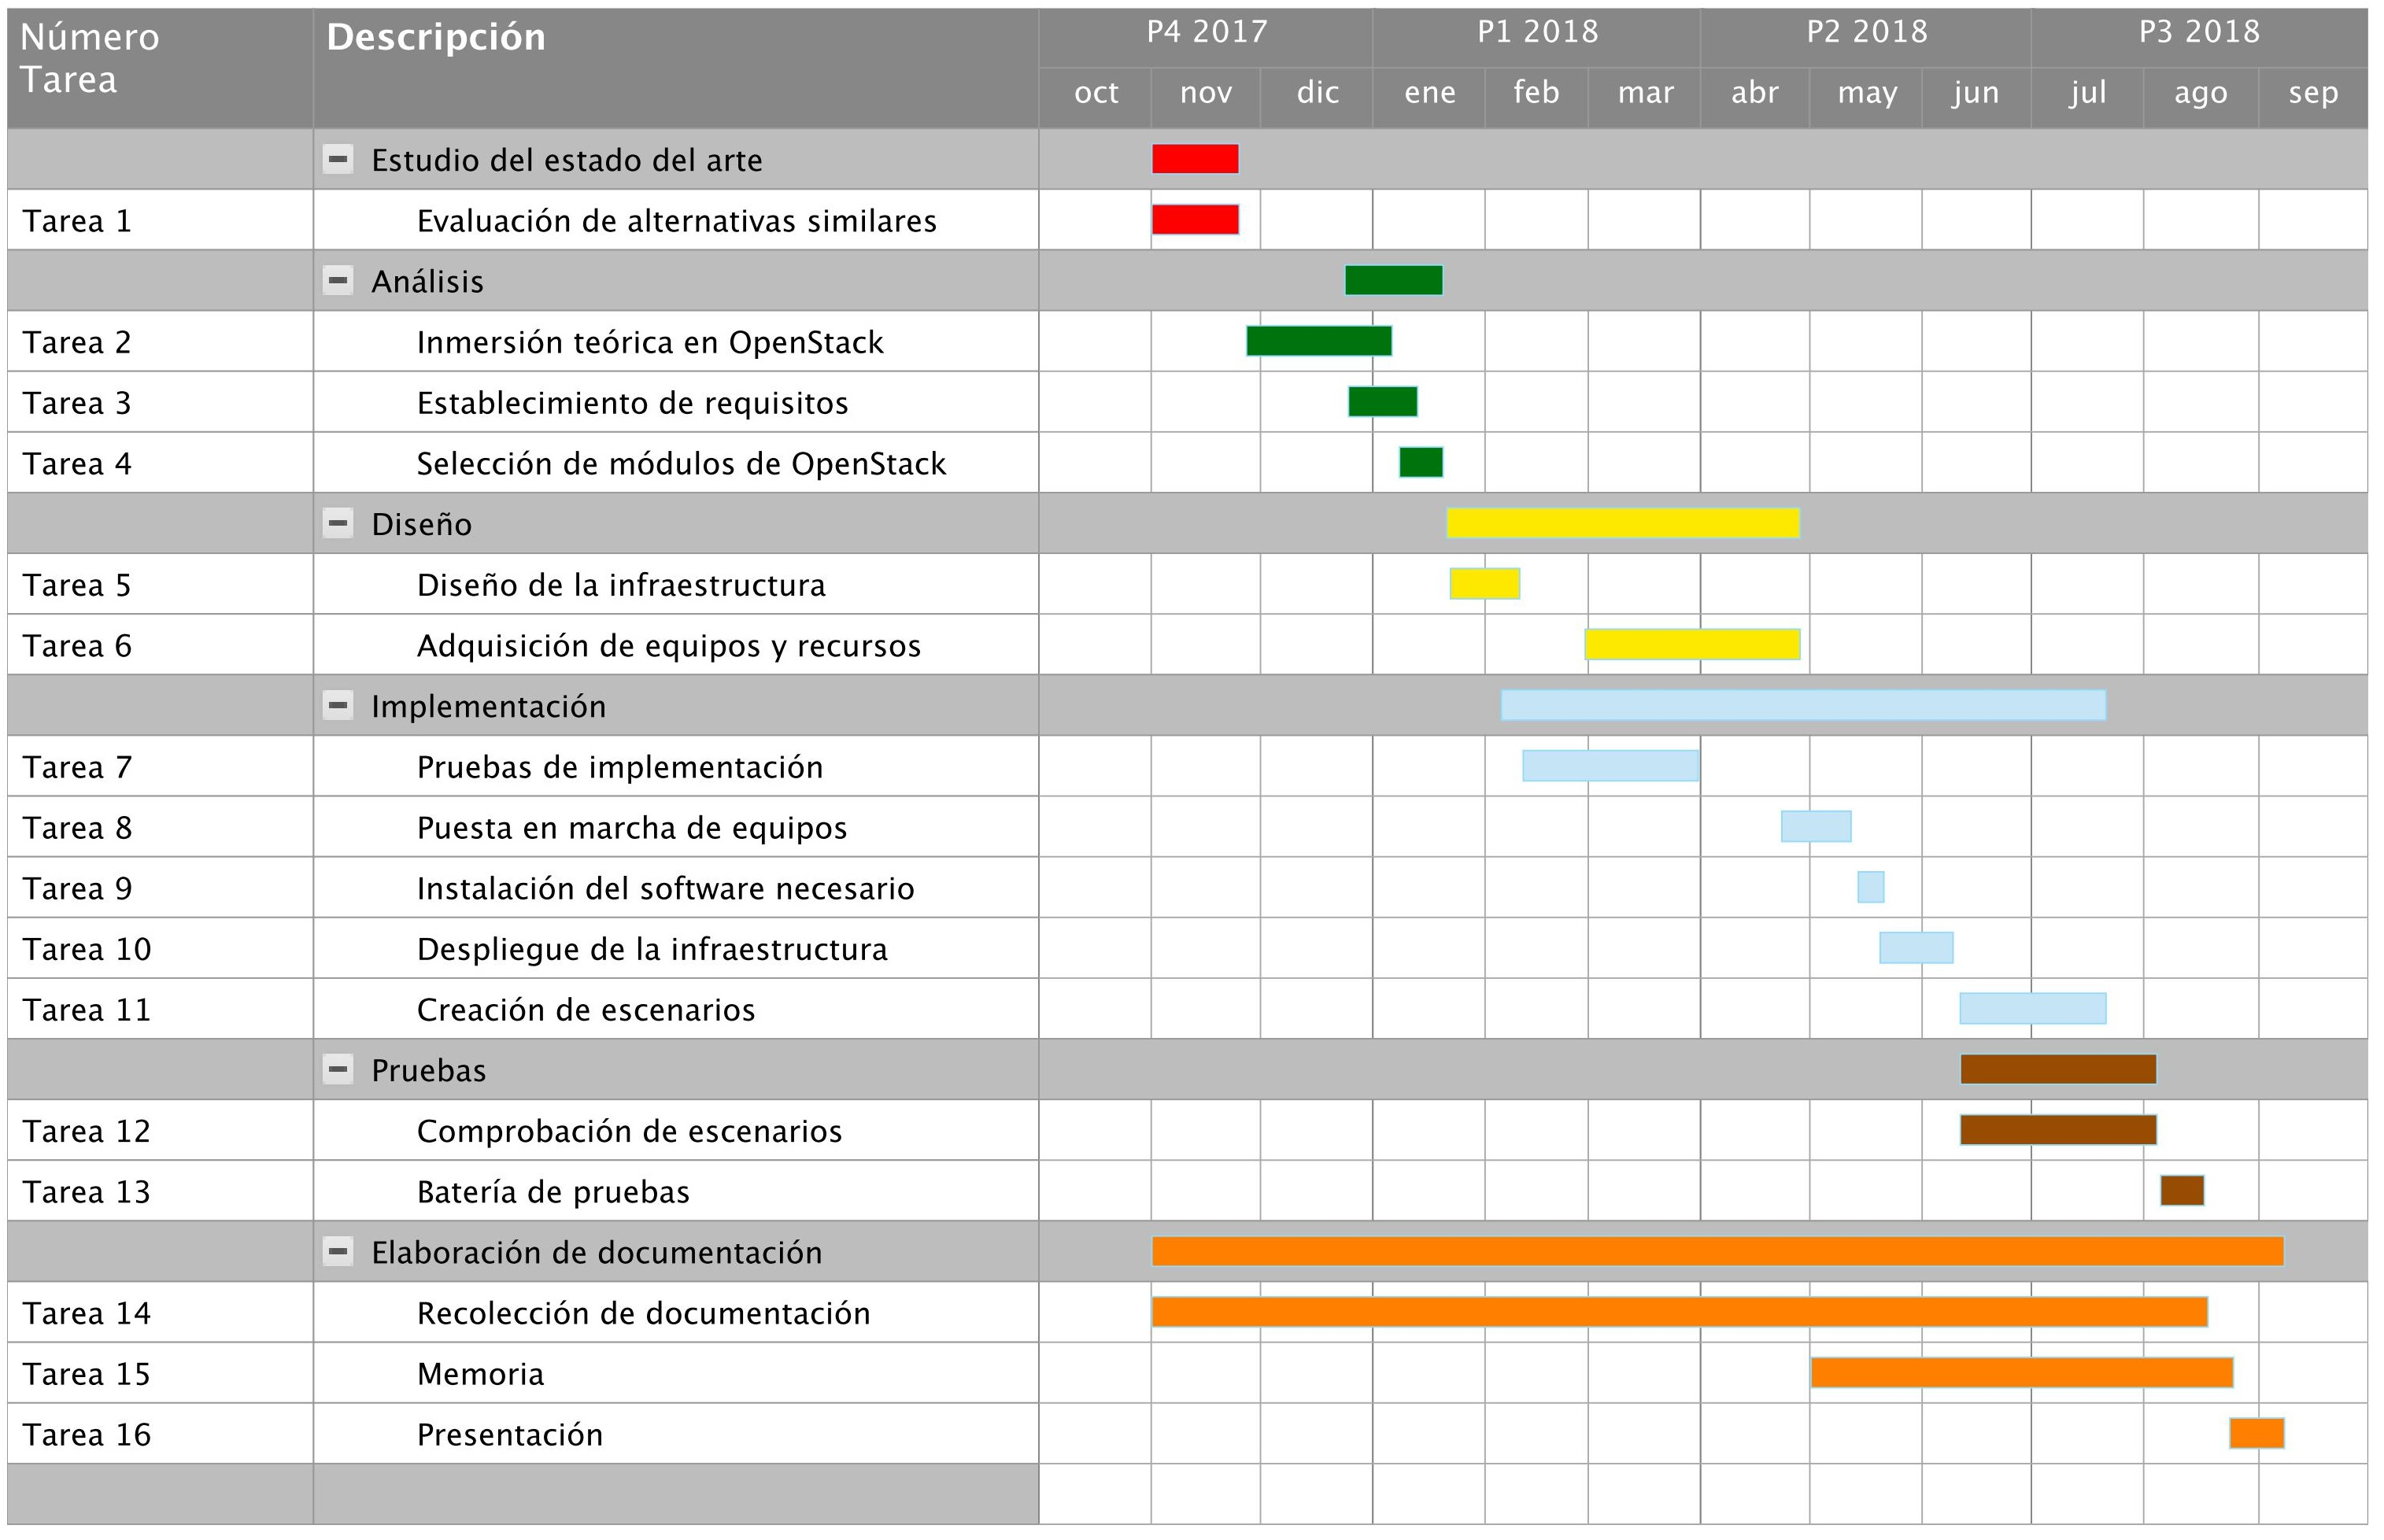
\includegraphics[width=1\textwidth]{imagenes/capitulo3/gantt-trimestral.jpg}
    \caption{Diagrama de Gantt trimestral.}
	\vspace{0.3cm}
    \label{fig:gantTrimes}
\end{figure}


\subsection{Estudio del estado del arte}
Dentro de esta primera fase, se evaluarán distintas alternativas similares a OpenStack para determinar si es la herramienta idónea para abordar el proyecto.

\subsection{Análisis}
Esta fase de análisis es vital, ya que nos servirá par adquirir un conocimiento profundo de OpenStack a nivel teórico así como definir los requisitos que necesitaremos para llevar a buen puerto este proyecto.

Una vez realizadas estas tareas tendremos el nivel necesario para decidir que módulos de OpenStack necesitamos instalar para poder gestionar métricas, alarmas, orquestación de funciones de red y otros.

En la memoria, el resultado de este apartado se ve reflejado a lo largo de todos los capítulos en los que se analizan distintos temas en función del apartado en el que nos encontremos.

\subsection{Diseño}
Ya definida la planificación de los requisitos, especificaciones y  módulos a estudiar para nuestro entorno IaaS, podemos diseñar la infraestructura de red que soportará nuestro servicio a nivel teórico.

En esta fase y en paralelo se irán adquiriendo los recursos hardware y software que necesitaremos tras el estudio de la fase anterior.

\subsection{Implementación}
Con todo a punto, en esta fase nos pondremos a desplegar el entorno con el que trabajaremos en OpenStack. Para ello en primer lugar se realizarán una serie de pruebas de instalación e implementación en un ordenador personal para una vez puesta en marcha los distintos equipos necesarios, poder instalar el software de OpenStack y realizar el despliegue de la infraestructura sea una tarea más ágil y precisa.

En este apartado se crearán también los distintos escenarios que justifican la elaboración de esta memoria.


\subsection{Pruebas}
El despliegue de la infraestructura finalizará con la comprobación del correcto funcionamiento de los distintos escenarios planteados en los que se harán una serie de pruebas para asegurarnos de que el entorno creado se comporta de acuerdo a las necesidades de orquestación de funciones de red que tenemos.

\subsection{Documentación}
Esta última fase comienza desde el principio de la elaboración del proyecto. Por un lado desde el inicio hasta prácticamente el final del proyecto se irá recolectando información y fuentes que iremos necesitando para superar las distintas fases aquí explicadas.

Se incluye aquí la realización tanto de la memoria técnica como de la presentación para la defensa final que se expondrá ante el jurado.

\section{Recursos}
En esta sección se hará un desglose en distintas subsecciones de los recursos que puedan estar implicados en este proyecto, tanto humanos como de hardware y software, facilitando así la estimación de costes en la sección posterior.

\subsection{Recursos humanos}
Los recursos humanos de este proyecto serán las personas implicadas en el mismo, a saber:

\begin{itemize}
\item D. Jorge Navarro Ortiz. Profesor titular de universidad del departamento de \textit{Teoría de la señal, telemática y comunicaciones} de la \textit{Universidad de Granada}. Tutor del presente trabajo fin de grado.
\end{itemize}

\begin{itemize}
\item Alejandro Toledo Juan. Estudiante del \textit{Grado en Ingeniería de Tecnologías de Telecomunicación} en la \textit{Escuela Técnica Superior de Ingenierías Informática y de Telecomunicación}, \textit{Universidad de Granada}. Autor del presente trabajo fin de grado.
\end{itemize}


\subsection{Recursos hardware}
Para la implementación del proyecto se requerirán los siguientes recursos hardware:
\begin{itemize}
\item Ordenador portátil Sony Vaio PCG-81112M con procesador Intel Core i7-4710HQ a 2,5 GHz, con una memoria RAM de 8 GB y disco duro de 500 GB. Este portátil será utilizado para la realización de pruebas de implementación de OpenStack antes de la instalación definitiva en los servidores.
\item Servidor 1. Asus G11 CD-K-SP012T. Procesador Intel Core i7-7700 a 3,6 GHz, con una RAM de 16 GB DDR4 y disco duro de 1TB más 128 GB SSD SATA3. Este servidor será el principal a la hora del desarrollo e implementación de nuestra nube.
\item Servidor 2. Acer G3-710. Procesador Intel Core i7-7700 a 3,6 GHz, con memoria RAM de 32 GB y disco duro de 1TB más 256 GB SSD. En este servidor se creará la segunda región de nuestra cloud que simulará un data center localizado en otro emplazamiento geográfico.
\item TP-LINK DGE-Tarjeta de Red Gigabit 10/100/1000. Tarjeta de red que se instalará en el segundo servidor para poder conectarse a Internet y permitir la conexión externa a través del primer servidor, ya que sólo dispondremos de una IP pública.
\item Cable RJ-45 Cat.5e. NANOCABLE: RJ45, Cat.5e UTP AWG24, latiguillo de 20 mts. Cable de red con latiguillo incluido de categoría 5e que usaremos para conectar los servidores entre sí y uno de ellos, el primero, a la toma de red que nos dará conexión a Internet.
\item Regleta APC P5BV-SP Regleta con Proteccion 5 Tomas y Coaxial 230V. Regleta que usaremos para conectar la alimentación de los servidores a la toma eléctrica.
\end{itemize}

\subsection{Recursos software}
Del mismo modo, he aquí el listado del software necesario para el desarrollo del TFG.
\begin{itemize}
\item Sistema operativo Ubuntu Server 16.04 LTS. Se ha optado por este sistema ya que es el aconsejado por los creadores de OpenStack para realizar la instalación all-in-one con Devstack y por el uso habitual del mismo durante el Grado y a nivel personal.
\item Openstack. El software necesario para la instalación de todos los componentes necesarios lo encontramos en los  repositorios de GitHub de all-in-one Devstack.\cite{noauthor_devstack:_2018}
\item Overleaf. Procesador de textos online gratuito basado en LATEX que usaremos para la redacción de la memoria.
\item Zotero. Herramienta para la gestión de referencias bibliográficas.
\item Smartsheet. Es un software online que nos permite diseñar diagramas de Gantt en distintos formatos.
\item Lucidchart. Esta herramienta disponible online, nos permite realizar todo tipo de diagramas: diagramas de red, diagramas de flujo, esquemas, diagramas UML...
\end{itemize}

\section{Estimación de costes}

\subsection{Costes humanos}\label{subchap:costeshumanos}
Actualmente en España no existe un salario de referencia para un profesional del sector\cite{noauthor_boe.es_nodate}, por tanto la estimación que aparece en la tabla \ref{tab:coste-recursos-humanos} se ha realizado en base a lo que suele cobrar un ingeniero de telecomunicaciones en función de su experiencia. Así, el precio por hora del trabajo en el proyecto realizado por Alejandro Toledo Juan, será de 20 \euro/hora mientras que el realizado por D.Jorge Navarro Ortiz y que se corresponde con las tutorías será de 50 \euro/hora. 

\renewcommand\arraystretch{1.1}
\begin{table}[!h]
\centering
\begin{adjustbox}{max width=\textwidth}
\begin{tabular}{|c|l|c|l|c|}
\hline
\textbf{Concepto} & \textbf{Precio/hora} & \textbf{Horas} & \textbf{Total}   \\
\hline \hline
Trabajo en el proyecto & 20 \euro/hora & 669 & 13380 \euro \\
\hline
Tutorías & 50 \euro/hora & 14 & 700 \euro \\
\hline
\multicolumn{3}{|l|}{\textbf{Total}} & \textbf{14080 \euro} \\
\hline
\end{tabular}
\end{adjustbox}
\caption{Estimación de costes de recursos humanos.}
\label{tab:coste-recursos-humanos}
\end{table}


\subsection{Costes hardware}
En la tabla \ref{tab:costes-hardware} se muestra un desglose de los costes de los recursos hardware. Para el coste de los servidores y el PC, se ha tenido en cuenta que el tiempo de vida útil está en torno a los 4 años, es decir, 48 meses. Se estima pues el coste de estos en el proyecto calculando la parte proporcional de ese coste para 5 meses que será el tiempo que se estima estén operativos:

Precio total del PC Portátil: 783.49\euro. Precio proporcional: 81.16\euro.
Precio total del Servidor 1: 1132.78\euro. Precio proporcional: 117.99\euro.
Precio total del Servidor 2: 1542.59\euro. Precio proporcional: 160.69\euro.
\renewcommand\arraystretch{1.1}
\begin{table}[!h]
\centering
\begin{adjustbox}{max width=\textwidth}
\begin{tabular}{|c|l|c|l|c|}
\hline
\textbf{Concepto} &  \multicolumn{1}{|c|}{\textbf{Descripción}} & \textbf{Cantidad}  & \textbf{Precio (\euro)}  \\
\hline \hline
PC Portátil & Sony Vaio: i7, 8 GB RAM  & 1 & 81.16 \\
\hline
Servidor 1 & Asus: i7, 16 GB RAM & 1 & 117.99 \\
\hline
Servidor 2 & Acer: i7, 32 GB RAM & 1 & 160.69 \\
\hline
Tarjeta Ethernet & TP-LINK DGE-Tarjeta de Red Gigabit 10/100/1000
 & 1 & 12.26 \\
\hline
Cable RJ-45 Cat.5e & NANOCABLE: RJ45, Cat,5e UTP AWG24, latiguillo de 20 mts
 & 2 & 13.56 \\
\hline
Regleta & APC P5BV-SP Regleta con Protección 5 Tomas y Coaxial 230V
 & 1 & 15.99 \\
\hline
\multicolumn{3}{|l|}{\textbf{Total}} & \textbf{402.11} \\
\hline
\end{tabular}
\end{adjustbox}
\caption{Estimación de costes de recursos hardware.}
\label{tab:costes-hardware}
\end{table}


\subsection{Costes software}
Como podemos ver en la tabla \ref{tab:costes-software} Todas las tecnologías que se pretenden usar en el proyecto están licenciadas bajo una licencia Open Source y por tanto no tienen ningún coste asociado.

\renewcommand\arraystretch{1.1}
\begin{table}[!h]
\centering
\begin{adjustbox}{max width=\textwidth}
\begin{tabular}{|c|l|c|l|c|}
\hline
\textbf{Concepto} &  \multicolumn{1}{|c|}{\textbf{Descripción}} & \textbf{Cantidad}  & \textbf{Precio (\euro)}  \\
\hline \hline
Sistema Operativo & Ubuntu Server 16.04 LTS
  & 3 & 0 \\
\hline
Openstack & All-in-one Devstack & 3 & 0 \\
\hline
Overleaf & Procesador de texto en LATEX online & 1 & 0 \\
\hline
Zotero & Gestor de referencias bibliográficas & 1 & 0 \\
\hline
Smartsheet & Diseño de diagramas de Gantt & 1 & 0 \\
\hline
Lucidchart & Diseño de diagramas  & 1 & 0 \\
\hline
\multicolumn{3}{|l|}{\textbf{Total}} & \textbf{0} \\
\hline
\end{tabular}
\end{adjustbox}
\caption{Estimación de costes de recursos software.}
\label{tab:costes-software}
\end{table}

\subsection{Costes de servicios}
Además de los costes ya citados, existen otros derivados de los servicios necesarios para el desarrollo de este trabajo y que tienen que entrar también en la planificación de gastos. Estos aparecen en la tabla \ref{tab:costes-servicios}. 

Vamos ahora a justificar la estimación de los mismos:

\begin{itemize}
\item Como podemos ver en la Fig.\ref{fig:tareas}, la puesta en marcha de los equipos comenzará el 23/04/18. En la puesta en marcha se contempla la solicitud de acceso al aula donde se han alojarán los equipos, de la IP pública necesaria para el acceso externo y la propia solicitud de los equipos hasta su posterior recepción. Se prevé disponer de los equipos ya instalados el 11/05/2018.

La desinstalación de la infraestructura  una vez finalizado el proyecto y la presentación, está planificada para el 14/07/2018. Esto hace un total de 127 días, o bien, 3048 horas.

En la tabla \ref{tab:costes-servicios} se ha calculado el precio de la luz teniendo en cuenta que el 11/05/2017, un año antes en la misma fecha que se prevé estén instalados los servidores, el precio medio de 1kWh era de 0.09808\euro/kW en Endesa.\cite{noauthor_endesa_nodate}

Mencionar que el precio se ha estimado en base al pico de potencia consumido por lo que será previsiblemente menor al que aparece.

\item Línea de acceso a Internet, que será la que nos permita la conexión remota y el acceso a la red externa en el entorno creado. La línea tiene un coste de 30\euro/mes y estará disponible durante 5 meses.
\end{itemize}


\renewcommand\arraystretch{1.1}
\begin{table}[!h]
\centering
\begin{adjustbox}{max width=\textwidth}
\begin{tabular}{|c|l|c|l|c|}
\hline
\textbf{Concepto} &  \multicolumn{1}{|c|}{\textbf{Descripción}} & \textbf{Consumo total(kW/h)}  & \textbf{Precio (\euro)}  \\
\hline \hline
Consumo energético & 2 servidores de 150 W  & 914.4 & 89.68\\
\hline
Internet & Línea de acceso durante 5 meses a 30\euro/mes &  & 150  \\
\hline
\multicolumn{3}{|l|}{\textbf{Total}} & \textbf{239.68} \\
\hline
\end{tabular}
\end{adjustbox}
\caption{Coste estimado de los servicios.}
\label{tab:costes-servicios}
\end{table}


\section{Presupuesto final}
\renewcommand\arraystretch{1.1}
\begin{table}[!h]
\centering
\begin{adjustbox}{max width=\textwidth}
\begin{tabular}{|c|l|}
\hline
\textbf{Concepto} & \textbf{Precio (\euro)}  \\
\hline \hline
Recursos humanos &  14080 \\
\hline
Recursos hardware & 402.11  \\
\hline
Recursos software & 0 \\
\hline
Servicios & 239.68 \\
\hline
\textbf{Total} & \textbf{14721.79} \\
\hline
\end{tabular}
\end{adjustbox}
\caption{Presupuesto final estimado.}
\label{tab:costes-final}
\end{table}

Una vez identificados todos los recursos que se van a utilizar y lo costes asociados a estos, podemos hacer un presupuesto final en el que aparecen todos ellos \ref{tab:costes-final}.

\jorge{Ten cuidado que te sales del margen}

Finalmente vemos que el coste total estimado del proyecto es de \textbf{14721.791\euro}, CATORCE MIL SETECIENTOS VEINTIUNO CON SETENTA Y NUEVE EUROS.
\chapter{Herramientas utilizadas} \label{chap:herramientasutilizadas}
En este capítulo vamos a ver los orígenes de OpenStack, de donde viene y como podemos contribuir con el proyecto. 

Después discutiremos el rol de la \textit{OpenStack Foundation} y cómo los diferentes grupos de OpenStack Foundation están trabajando juntos para hacer de OpenStack la solución en la nube más importante de nuestros días. 

Además veremos una descripción general de alto nivel de OpenStack y estudiaremos como usar OpenStack para hacer que la administración de la infraestructura de IT sea más flexible. 

Para ello, iremos tratando los diferentes proyectos de OpenStack que forman el núcleo de proyectos principales, como son Nova, Neutron, Glance o Cinder entre otros. 

Listaremos también otros proyectos y servicios importantes de OpenStack haciendo énfasis finalmente en aquellos relevantes para la orquestación de NFVs y la consecución de nuestros objetivos.

\section{Orígenes de OpenStack}
OpenStack comenzó en 2010, como un proyecto conjunto de \textit{Rackspace Hosting} y \textit{NASA (National Aeronautics and Space Administration)}. La NASA contribuyó con su plataforma \textit{Nebula}, que luego se convirtió en \textit{Nova}. Rackspace contribuyó con su plataforma \textit{Cloud Files}, que más tarde acabó derivando en  en \textit{Swift}.

En abril de 2011, se produjo el lanzamiento de \textit{OpenStack Bexar} en Ubuntu. Más tarde ese mismo año, Debian incluyó \textit{OpenStack Cactus} en su distribución. En 2012, Red Hat anunció una vista previa de su distribución OpenStack también. Desde entonces, muchos otros le siguieron, incluyendo Oracle, HP y Vmware.

\section{OpenStack Foundation}
\textit{The OpenStack Foundation}, es una fundación que promueve el desarrollo global, la distribución y la adopción del sistema en la nube, proporcionando recursos compartidos para hacer crecer la nube de OpenStack. También permite a los proveedores de tecnología y desarrolladores ayudar en la producción de software en la nube. \cite{noauthor_foundation_nodate}

Existen dentro del gran número de de empresas que conforman la \textit{OpenStack Foundation} distintos estatus según el tipo de rol que tengan como miembros. Dependiendo del rol pueden tener una participación mayor o menor en el abastecimiento de fondos para capacitar y promover la comunidad y el software de OpenStack además de encargarse de la gestión del proyecto. Entre las empresas que participan se encuentran Intel, Huawei, Rasckpace, RedHat, SUSE, Mirantis, Cisco, Citrix, Lenovo, Juniper y un sin fin de compañías más.\cite{noauthor_companies_nodate}


\section{El Core de los proyectos en Openstack}
OpenStack incluye numerosos proyectos, cada uno de ellos con un estado de adopción diferente. Al mismo tiempo, se están agregando nuevos proyectos de forma regular.
Si deseamos aprender acerca de OpenStack, es importante familiarizarse con los diferentes productos que existen. Dos veces al año, la \textit{OpenStack Summit} toma  decisiones sobre la implantación de nuevos proyectos, por lo que se están agregando nuevos proyectos de forma regular.

En el sitio web de OpenStack \cite{noauthor_open_nodate}, se puede obtener una visión general actualizada de todos los proyectos que existen. OpenStack Foundation distingue entre servicios principales y servicios opcionales. Los servicios principales que forman el core son \textit{Nova, Neutron, Swift, Cinder, Keystone y Glance}. Una de las cosas interesantes que podemos ver en la web, es la adopción actual. Así, por ejemplo, vemos como Nova es una parte esencial de OpenStack, porque el 93\% de todas las nubes OpenStack lo usan.


También podemos ver que hay servicios opcionales, y algunos de ellos bastante usados en los despliegues de OpenStack, como es el caso de \textit{Horizon}, por ejemplo, que existe desde hace 7 años y lo adoptan el 86\% de todas las implementaciones de OpenStack. Pero también surgen constantemente nuevos servicios como \textit{Magnum} y \textit{Congress}. Por tanto, para cualquier servicio, si vemos los detalles de ellos, podremos ver información sobre los mismos en la wiki del proyecto, indicadores de uso, puntuación, o si es un proyecto que está comenzando o ya maduro.

\begin{figure}
    \centering
    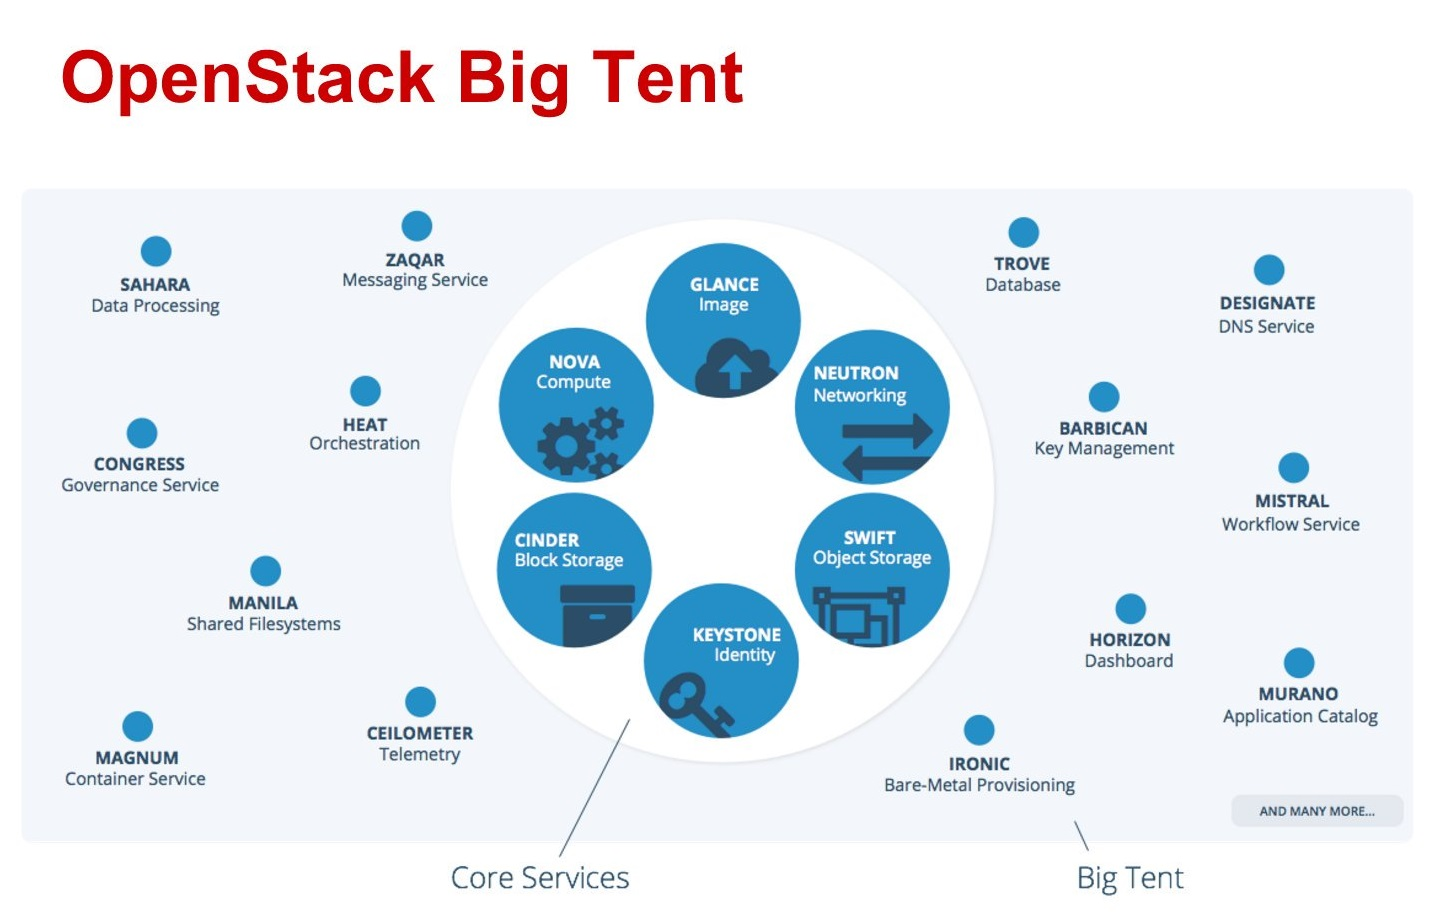
\includegraphics[width=0.7\textwidth]{imagenes/capitulo4/bigtent.png}
    \caption{Big Tent and Core Services.}
	\vspace{0.3cm}
    \footnotesize{Fuente: OpenStack}
    \label{fig:bigtent}
\end{figure}


Actualmente existen una serie de servicios dentro de OpenStack conocidos como \textit{Big Tent and Core Services} que podemos ver en la Fig.\ref{fig:bigtent} entre los que se encuentran el núcleo de servicios de Openstack antes citados, y otros servicios que son habituales encontrar en los despliegues de OpenStack y que varían en función del uso que se le vaya a dar a la infraestructura. 

Estos servicios junto a otros relevantes se describen en los siguientes apartados. Además en el anexo \ref{chap:arquitectura} podemos ver el esquema lógico de OpenStack con los componentes y relación que existe  entre la mayoría de proyectos que trataremos.

\subsection{Núcleo de servicios}

\begin{tcolorbox}[colback=orange!5!white,colframe=orange!75!black]
Jorge: Si no me equivoco, las SDN dadas por Nova son para crear las redes entre máquinas virtuales y hacia el exterior, ¿verdad? Coméntalo, porque, tal como lo pones ahora, da la sensación de que OpenStack también sirva para implementar redes SDN, y esa no es su función.
\end{tcolorbox}

\begin{itemize}
\item \textbf{Nova Compute}. Es la interfaz para el hipervisor. Se asegura de que las máquinas virtuales se puedan ejecutar en algún lugar de la nube.
\end{itemize}

\begin{itemize}
\item \textbf{Neutron Networking}. Proporciona redes definidas por software (\textit{Software Defined Networks}, SDN) en la nube a través del uso de switches software \textit{Open vSwitch}.
\end{itemize}
%Neutron es un proyecto de OpenStack usado para proporcionar conectividad de red como un servicio.

\begin{itemize}
\item \textbf{Swift Object Storage}. Con Swift podemos usar el almacenamiento en la nube de una forma inteligente, un almacenamiento que no esté vinculado a dispositivos físicos, sino que se organice en objetos binarios que se pueden dispersar por toda la nube de una manera distribuida y replicada.
\end{itemize}

\begin{itemize}
\item \textbf{Cinder Block Storage}. Como administradores, podemos usarla para proporcionar almacenamiento persistente a la máquina virtual que estamos implementando en la nube.
\end{itemize}

\begin{itemize}
\item\textbf{Keystone Identity}. Keystone nos permite combinar todo lo anterior. Podemos crear usuarios, roles o perfiles y servicios. Con esta herramienta definiremos que usuario tiene acceso a qué servicio específico y cómo los servicios específicos pueden comunicarse entre sí.
\end{itemize}

\begin{itemize}
\item \textbf{Glance Image}. Es el servicio de imágenes, necesario para implementar una instancia de una imagen en la nube. 
\end{itemize}

\subsection{Nova}
Nova es quizás el proyecto principal más importante en OpenStack \cite{noauthor_nova_nodate}. Este proyecto es el responsable de administrar el ciclo de vida de las instancias de cómputo. Ahora bien, ¿qué es una instancia de cómputo? El término de cómputo del inglés \textit{compute} es simplemente otro nombre para Nova, que podrá ser cualquier equipo o servidor en el que esté instalado el servicio y una instancia es una máquina virtual, por tanto, Nova se encarga de ejecutar la máquina virtual. 

Para ello, Nova se conecta al hipervisor pero no es el hipervisor en sí mismo. Esto lo hace muy interesante ya que independientemente del hipervisor que se esté ejecutando, bien sea Xen, KVM, VMware, vSphere o cualquier otro, Nova lo puede tratar. 
Nova instalará un agente en el hipervisor para asegurarse de que sea compatible con nuestro entorno OpenStack y se hará responsable de crear, planificar y  desmantelar las máquinas virtuales bajo demanda, incluyendo los procesos del servicio Nova que se ejecutan en el controlador de la nube, así como los agentes Nova, que se ejecutan en el hipervisor.

\subsection{Neutron}\label{subsec:Neutron}
El siguiente proyecto central de OpenStack es \textit{Neutron}. Neutron posibilita la creación de redes definidas por software. Las SDN permiten a los usuarios definir su propia red para las instancias que se implementen.\cite{noauthor_neutron_nodate}

\begin{figure}
    \centering
    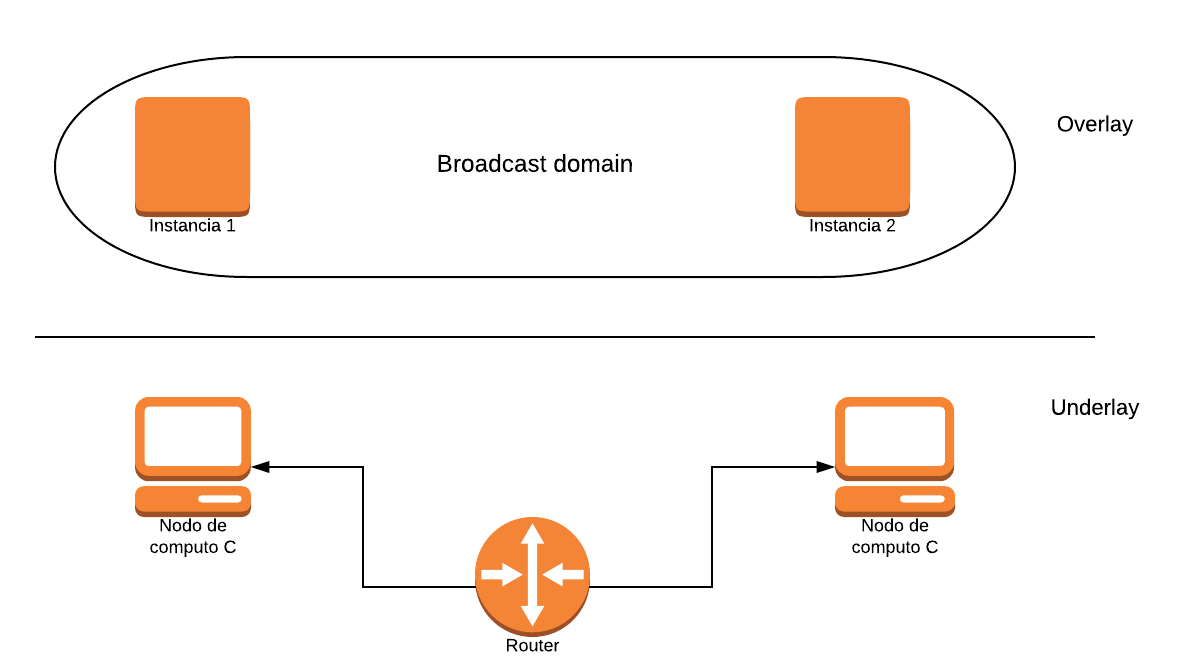
\includegraphics[width=0.7\textwidth]{imagenes/capitulo2/sdn_openstack.png}
    \caption{SDN en Openstack.}
	\vspace{0.3cm}
    \label{SDN en Openstack}
\end{figure}

Imaginemos un entorno típico de OpenStack como el de la Fig.\ref{SDN en Openstack}. En este supuesto entorno hay dos nodos C de cómputo diferentes. Estos nodos se conectarán mediante el uso de una red física que simulamos como un router en la figura. Llamamos a esta parte, la red subyacente , \textit{underlay network}. En esta red física se realizará enrutamiento y lo necesario para que funcione. Esta parte de la configuración de la red física será típicamente lo que el usuario de OpenStack no conocerá.

El nivel de usuario, que será el nivel más alto, es lo que llamaremos la red de superposición o \textit{network overlay}. En el nivel de usuario, puede haber distintas instancias ejecutándose en lugares diferentes (instancias 1 y 2 ejecutándose cada una en un nodo), pero el usuario puede desear implementar estas instancias como si se usaran en el mismo dominio de difusión (\textit{broadcast domain}), formando así una red lógica.

En un dominio de difusión, las instancias estarán en la misma red, por lo que, ¿cómo puede ser que estén en el mismo dominio de difusión si en la red subyacente tenemos diferentes redes físicas? Esto es exactamente de lo que Neutron se está ocupando mediante el uso de redes definidas por software. Para hacerlo, Neutron necesita interconectar la arquitectura de la red física, para lo cual utiliza una arquitectura conectable (\textit{pluggable architecture}). Esta arquitectura conectable admite muchos proveedores y tecnologías de redes. Por lo tanto, si se ha realizado una gran inversión en alguna tecnología de red patentada, es probable que haya un buen plugin de Neutron disponible. La mayoría de los proveedores de red tienen plugins de Neutron, por lo que no tendremos por norma general problemas con esto.

Además, Neutron proporciona una API para que los usuarios definan las redes y los archivos adjuntos en ellas. Como resultado, para un programador o administrador será relativamente sencillo crear su propio entorno de SDN, como veremos más adelante.

\subsection{Swift}
El siguiente proyecto central de OpenStack del que hablaremos es \textit{Swift}. Swift está diseñado para proporcionar escalabilidad en el nivel de almacenamiento. Funciona con objetos binarios para almacenar datos de una manera distribuida y replicada. \cite{noauthor_swift_nodate}

El almacenamiento finalmente termina en un disco duro y un disco duro es un dispositivo físico. El problema con los dispositivos físicos es que son limitados y no son muy escalables, por lo que si todo nuestro almacenamiento en la nube estuviese en un servidor que proporciona diferentes discos duros, no tendríamos escalabilidad. Para tenerla, Swift ofrece un modelo de almacenamiento basado en objetos.

\begin{figure}
    \centering
    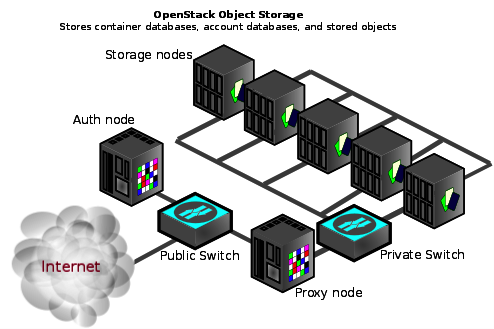
\includegraphics[width=0.7\textwidth]{imagenes/capitulo2/swift_storage.png}
    \caption{Almacenamiento de objetos distribuido con Swift.}
    \footnotesize{Fuente: Mirantis}
	\vspace{0.3cm}
    \label{Swift Storage}
\end{figure}

Para entender el funcionamiento de Swift nos fijaremos en la Fig.\ref{Swift Storage}. La idea sobre Swift es que tenemos una aplicación que usaremos para escribir datos. En un entorno OpenStack, la aplicación no escribe un archivo en el disco duro, sino que esta puede interactuar con el almacenamiento de objetos de Swift que  se está comunicando a su vez con muchos nodos de almacenamiento.

En la Fig.\ref{Swift Storage} podemos ver distintos nodos de almacenamiento (\textit{Storage nodes}). Swift está usando un proxy y cuando el proxy de Swift recibe datos de la aplicación, va a crear objetos binarios. Estos objetos binarios son los fragmentos de datos.

Digamos que tenemos objetos binarios A, B y C. En Swift, el objeto binario A se puede almacenar en uno de los nodos de almacenamiento, el objeto binario B en otro y el C en otro diferente. Si solo se almacena una vez, el sistema no será tolerante a fallos, por lo que Swift incluye un algoritmo de replicación para almacenar los objetos binarios en múltiples nodos. Por defecto, esto se hará tres veces, es decir, cada objeto se almacenará en tres nodos diferentes, aunque podríamos almacenarlo en un número mayor de nodos si así lo requerimos.

Este proceso hace que el almacenamiento sea más eficiente ya que en el momento en que la aplicación necesita recuperar los datos, se dirigirá al proxy Swift nuevamente y el proxy Swift estará utilizando un algoritmo avanzado para determinar exactamente dónde residen los objetos binarios, enviando llamadas a todos los nodos de almacenamiento involucrados. Debido a todos estos nodos de almacenamiento que podrán funcionar en paralelo, los datos llegarán al proxy de Swift, y por lo tanto, a la aplicación, de una manera muy rápida. Y así es como se consigue con OpenStack hacer que el almacenamiento sea escalable.

Aún tiene más ventajas, imaginemos que estos nodos de almacenamiento son de un terabyte cada uno. Cuando nos estamos quedando sin almacenamiento disponible, es bastante fácil agregar un par de nodos de almacenamiento Swift más, e incluso se pueden reequilibrar los objetos binarios que están escritos en la configuración de almacenamiento de Swift.

La aplicación que se usa para hablar con Swift, está utilizando una API RESTful.
REST es una forma estándar de comunicación en un entorno OpenStack como ya sabemos. Esto significa que la aplicación no está escribiendo un archivo en un sistema de archivos, sino que está utilizando una llamada RESTful API, que es entendida por Swift proxy. La API RESTful es el lenguaje nativo de OpenStack, y eso convierte a Swift en la opción nativa para el almacenamiento de objetos en OpenStack.

\subsection{Glance}
El siguiente proyecto importante de OpenStack es Glance. Glance se usa para almacenar imágenes de disco de la máquina virtual\cite{noauthor_glance_nodate}. Las máquinas virtuales, que son las instancias, no están instaladas, sino que se generan a partir de una imagen que podemos descargar\cite{noauthor_get_nodate}. Es como arrancar Linux desde un live CD. Las imágenes se pueden descargar fácilmente o se pueden crear para que coincidan con las necesidades específicas dentro de una organización.

En la web se proporcionan diferentes imágenes en la nube para diferentes sistemas operativos, que incluyen CentOS, Debian, Fedora, básicamente, todas las principales distribuciones de Linux, e incluso incluye Microsoft Windows.

Una imagen interesante es la imagen de CirrOS y lo es porque es muy pequeña, solo de trece megabytes, motivo por el cual la usaremos para realizar nuestros despliegues posteriormente debido a la limitación principalmente de RAM de nuestro entorno.

Así pues, Glance es como nuestra tienda de imágenes. Esto significa que si un administrador desea iniciar una instancia, iniciará la instancia desde el almacén de imágenes de Glance y es por ello que Glance es un pilar básico de OpenStack.

Para que todo sea escalable, el almacén de imágenes de Glance normalmente usa el almacenamiento de objetos Swift como un back-end. Por supuesto no hay porque utilizar el almacenamiento de objetos de Swift, pero usarlo lo hace más escalable. La otra opción sería usar el almacenamiento local como back-end para Glance, pero estariamos usando entonces almacenamiento local y por tanto vinculado a un servidor físico que contiene las imágenes física y que no es muy escalable.

\subsection{Cinder}
El siguiente proyecto esencial de OpenStack es Cinder\cite{noauthor_openstack_nodate-6} encargado de proporcionar almacenamiento persistente a las instancias. 

Por defecto, el almacenamiento de las instancias es efímero.  Es también como arrancar desde un live CD en Linux. Si trabajamos desde un live CD e intentamos cambiar el archivo de configuración, ¿dónde se cambiaría? porque la imagen del live CD está cargada en la RAM y realmente no existe en ningún disco duro grabable.

Este es el mismo problema que tenemos con las imágenes de Glance, y es por eso que en OpenStack, el almacenamiento instantáneo es efímero. Cinder es lo que permite a los administradores asignar almacenamiento persistente a las instancias.

Cinder también puede usar diferentes backends. Puede ser un almacenamiento local, que de forma predeterminada será LVM de Linux (\textit{Linux Volume Manager}) o puede incluir almacenamiento de objetos Swift y Ceph, incrementando así la escalabilidad.

\subsection{Keystone}
\begin{figure}
    \centering
    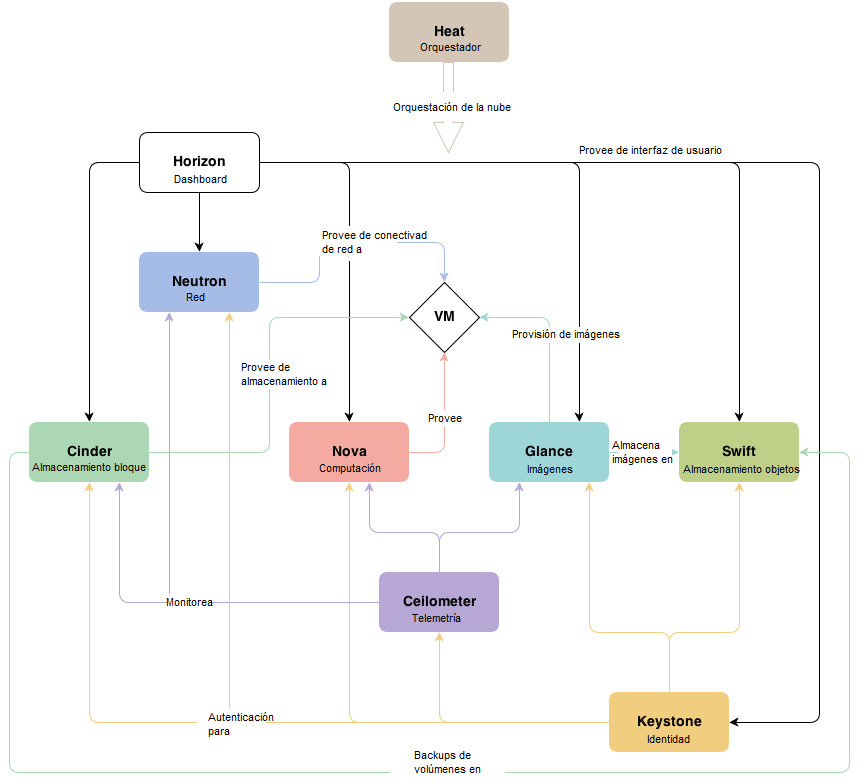
\includegraphics[width=0.7\textwidth]{imagenes/capitulo4/arquitectura1.png}
    \caption{Arquitectura conceptual de OpenStack.}
	\vspace{0.3cm}
    \footnotesize{Fuente: Daniel Romero Sanchez, “Openstack desde cero - Keystone”, DBigCloud, 2015} 
    \label{arquitecturaOpenStack}
\end{figure}

Ninguna nube OpenStack podría existir sin los servicios proporcionados por el proyecto Keystone. Keystone se usa para la autenticación, autorización y enumeración de todos los servicios y backends.\cite{noauthor_keystone_nodate}

Con servicio nos referimos en este caso a cualquiera de los proyectos que se implementa en OpenStack. De este modo, si queremos poder ejemplo acceder a Nova, Nova debe definirse como un servicio en Keystone y el backend proporciona una URL que da acceso al servicio específico. Como administradores, también podremos consultar estos servicios y backends como veremos.

Keystone es un elemento central en OpenStack tal como refleja la Fig.\ref{arquitecturaOpenStack} donde aparecen los principales proyectos de OpenStack que hemos ido enumerando y las relaciones comentadas que existen entre ellos.

En Keystone, los usuarios y roles se crean y se asignan a proyectos, que también se conocen como \textit{tenants}. Un proyecto, también conocido como tenant, por lo general, es un cliente de OpenStack. Si OpenStack se usa como una nube pública, pueden ser diferentes empresas que están contratando espacio en la nube en OpenStack y para distinguir entre los recursos disponibles para un cliente y otro cliente, OpenStack está utilizando esta noción de proyectos o tenants.

En un entorno de proyecto, normalmente se crearán cuentas de usuario a las que se asignarán roles específicos y dependiendo del rol asignado a una cuenta de usuario, los usuarios tendrán más o menos opciones para hacer cosas en OpenStack.

De todo ello se ocupa Keystone, por lo tanto, Keystone es un repositorio central para todos los servicios y resultados de backends.

De forma predeterminada, Keystone está utilizando una base de datos, que es la base de datos MariaDB (derivada de MySQL), para almacenar información, lo cual no significa que no podamos cambiarla a otras que queramos usar como OracleDB o bien, usar un directorio LDAP.

\subsection{\textit{The big tent}}
Otros proyectos interesantes de OpenStack que no forman parte de los principales pero que tienen un alto índice de adopción son:

\begin{itemize}
\item \textbf{Ceilometer.} Ceilometer es conocido como el servicio de telemetría y se usa para medición y registro. Recopila datos que pueden ser consultados por un software de terceros, pero también se pueden usar para obtener estadísticas de uso que se pueden pasar al servicio de Heat. Según la información que obtiene de Ceilometer, Heat puede ampliar o reducir automáticamente la cantidad de recursos en la nube.\cite{noauthor_celiometer_nodate}

\item\textbf{Trove.} Trove es un Database as a Service para OpenStack. Provee a OpenStack de motores de bases de datos relacionales y no relacionales. Su objetivo es ofrecer la funcionalidad de base de datos a los usuarios sin la necesidad de ocuparse de tareas de administración complejas. Como resultado, los usuarios así como los administradores pueden implementar instancias de base de datos fácilmente.\cite{noauthor_trove_nodate}

\item \textbf{Sahara.} Sahara es Big Data en OpenStack. Está configurado para ofrecer una fácil implementación de Hadoop sobre OpenStack. Sahara se ocupa de los parámetros de Hadoop, como la versión, la topología del clúster y el hardware. El usuario proporciona estos parámetros y Sahara implementará automáticamente el clúster. Sahara puede agregar y eliminar nodos fácilmente al clúster según sea necesario.\cite{noauthor_sahara_nodate}

\item \textbf{Ironic.} Ironic es el programa de aprovisionamiento  bare metal de OpenStack y fue desarrollado para implementar máquinas físicas (y no máquinas virtuales). Ironic es una API bare metal de hipervisor con un conjunto de complementos que interactúan con los hipervisores de bare metal. Utiliza PXE (\textit{Preboot Execution Enviornment}) o IPMI (\textit{Intelligent Platform Management Interface}) para aprovisionar y encender máquinas o apagarlas. Ironic también funciona con complementos específicos del proveedor para aportar funcionalidades adicionales.\cite{noauthor_ironic_nodate}


\item \textbf{Zaqar.} Zaqar es el servicio de mensajería OpenStack. Es una alternatia a una instalación independiente del servicio de mensajería AMQP (\textit{Advanced Message Queuing Protocol}) o ZeroMQ. Zaqar puede usar una API REST basada en HTTP, así como una API basada en websocket para la comunicación. Zaqar permite el manejo de colas de múltiples usuarios y proporciona una alta disponibilidad interna y escalabilidad, lo cual es un reto en los servicios de mensajería independientes.\cite{noauthor_zaqar_nodate}

\item \textbf{Manila.} Originalmente está basado en Cinder. Manila es el servicio de sistema de archivos de OpenStack. Ofrece una alternativa al almacenamiento local o de objetos, proporcionando así una solución de almacenamiento flexible.\cite{noauthor_manila_nodate}

\item \textbf{Designate.} El proyecto Designate proporciona DNS como servicio para OpenStack: acceso a API REST para administración de dominios y registros, utilizable en entorno multi-tenant, integrado con Keystone para autenticación, se integra con Noa y Neutron para la generación automática de registros DNS y soporte nativo para Bind9 y PoweDNS.\cite{noauthor_designate_nodate}

\item \textbf{Barbican.} Barbican implementa seguridad y administración de claves en la nube, proporcionando una API REST. Está diseñado para almacenamiento, aprovisionamiento y administración de todo tipo de claves, incluidas contraseñas, claves de cifrado y certificados X.509.\cite{noauthor_barbican_nodate}

\item \textbf{Magnum.} El proyecto Magnum fue desarrollado para permitir la administración de contenedores en OpenStack.  Su objetivo es integrar los motores de orquestación de contenedores como recursos de primera clase en OpenStack. Un ejemplo importante de este tipo de motor es Kubernetes: Magnum permite integrar Kubernetes en un entorno OpenStack para que pueda ejecutar contenedores orquestados de Kubernetes encima de OpenStack. El resultado es que se pueden integrar contenedores en OpenStack de manera similar a como las instancias se integran encima de Nova.\cite{noauthor_magnum_nodate}

\item \textbf{Murano.} El proyecto Murano proporciona un catálogo de aplicaciones para OpenStack. El objetivo de este proyecto es permitir que los desarrolladores de aplicaciones y los administradores de la nube publiquen las aplicaciones disponibles en un catálogo. Esto permite a los usuarios consultar una lista de aplicaciones en la nube de una manera fácil de navegar.\cite{noauthor_murano_nodate}

\item\textbf{Congress.} Congress es un proyecto de Policy as a Service. Proporciona gobernanza y cumplimiento como servicios en la nube. El administrador puede definir políticas y Congress se encargará de implementar estas políticas.\cite{noauthor_congress_nodate}

\item\textbf{Heat.}  Se usa para desplegar un conjunto de instancias en un entorno OpenStack. Esto nos permite desplegar múltiples máquinas virtuales relacionadas de una manera sencilla. Heat usa HOT (Heat Orchestration Template) o AWS CloudFormation template para definir las pilas o conjuntos de instancias orquestando de esta forma el resto de proyecto (ver Fig.\ref{arquitecturaOpenStack}). Este proyecto lo trataremos en detalle en la sección \ref{subchap:heat}.
\end{itemize}

\subsection{Detrás de los proyectos de OpenStack}
Detrás de todos estos servicios de OpenStack que forman el núcleo básico, también hay algo más. Siempre se requieren algunos servicios vitales y estos incluyen:

\begin{itemize}
\item La sincronización de tiempo o \textit{timestamp}. Esta es necesaria porque muchos servicios están utilizan timestamps para la comunicación, por ejemplo en Keystone. Keystone está enviando tickets que se basan en timestamps y si los servicios no llegan a un acuerdo en el momento adecuado, entonces, no habrá comunicación.
\item Otro servicio es la base de datos de MariaDB de la que hemos estado hablando cuando hablamos sobre Keystone, usada para almacenar toda la información relacionada con la nube. Esto es muy interesante porque como administradores, podremos consultar la base de datos y obtener información sobre lo que está sucediendo fuera de ella.
\item También está la cola de mensajes o \textit{message queue}. La cola de mensajes es un componente esencial al que los servicios acceden para intercambiar mensajes de forma ordenada entre los distintos servicios necesarios. Es como un servidor de correo SMTP en el manejo del correo electrónico, un servicio que se encarga de entregar el mensaje al destino correcto. Openstack incorpora AMQP como servicio de mensajería, siendo el agente predeterminado RabbitMQ.
\end{itemize}

En una implementación de OpenStack que está automatizada, todo esto se creará automáticamente. Si por contra optamos por implementar OpenStack manualmente, deberemos encargarnos nosotros mismos de estos tres servicios esenciales.

\section{La API RESTful}

Para comprender OpenStack, hay que entender el funcionamiento de la \textit{API RESTful}. REST es un método genérico para proporcionar acceso a todos los componentes de OpenStack. Todas las APIs de OpenStack son RESTful, lo que proporciona un acceso uniforme. Esto facilita el trabajo para los desarrolladores, ya que se usan los mismos estándares en todas partes y un desarrollador puede usar el mismo lenguaje en todo lo que hace.

El acceso a la API RESTful se puede utilizar al implementar comandos, pero también directamente usando curl, un proyecto de software consistente en una biblioteca (\textit{libcurl}) y un intérprete de comandos (\textit{curl}) orientado a la transferencia de archivos y que soporta protocolos como FTP, FTPS, HTTP, HTTPS, TFTP, SCP, SFTP, Telnet, DICT, FILE y LDAP entre otros.\cite{noauthor_curl_nodate}

Vamos a hacer una pequeña demostración de lo que la API RESTful hace posible.
Imaginemos que estamos en una máquina OpenStack. En la máquina OpenStack, podemos usar un comando como este:

\begin{lstlisting}[style=Consola]
stack@jorge-All-Series:/opt/stack# curl -s -X POST http://192.138.4.201:5000/v2.0/tokens -H "Content-Type: application/json" -d ' ("auth": {"tenantName": "'"$OS_TENANT_NAME"'", "passwordCredentials": {"username": "'"$OS_USERNAME"'", "password": "'"$OS_PASSWORD"'"}}}' | python -m json.tool
\end{lstlisting}

De este modo, estamos haciendo una llamada a la API de forma directa. Como administradores, no nos interesará hacer esto, pero es una forma de exponer lo que sucede detrás de la interfaz web de Horizon, o de la línea de comandos.

Al usar este comando, estamos accediendo a un endpoint de la API utilizando el método POST, por lo que, estamos haciendo un POST a tokens y estamos especificando en el content-type que el tipo de datos sea json, proporcionando además  credenciales de autenticación. Por último, redirigimos el resultado a Python, que está utilizando la herramienta json.

Como resultado obtendremos:

\begin{lstlisting}[style=Consola]
          ],
          "endpoints links": [],
          "name":"Image Service",
         "type":"image"
     },
          "endpoints": [
                {
                    "adminURL:"http://10.5.1.201:35357/v2.0",
                    "id":"5797558684004446bbe92448ffd3f6fw",
                    "internalURL":"http://10.5.1.201:5000/v2.0"
                    "publicURL":"http://10.5.1.201:5000/v2.0"
                    "region":"RegionOne"
                }
            ],
           "endpointss_links": [],
           "name":"keystone",
           "type":"identity"
     }
],
"token":{
    "audit_ids": [
          "3RAGfK16Ssui3kA6M2Cgmg"
      ],
     "expire":"2018-07-28T14:51:152",
     "id":"bb9ad8edda2e434a9b261c539a8bf1ea",
     "issued_at":"2018-07-28T14:51:152.86034ZZ",
     "tenant": {
           "description":"deafult tenant",
           "enabled":"true",
           "id":"7db988ced11842e3af279aaa2425f362",
           "name":"demo"
       }
},
"user": {
     "id":"ae8380b700344341994183c0cd6db4f9",
     "name":"demo",
     "roles": [
            {
                "name": "_member_"
            }
       ],	
      "roles_links": [],
      "username": "demo"
\end{lstlisting}

Esta es la información en crudo que OpenStack proporciona al administrador. Más adelante veremos la existencia de una línea de comandos que hace que esta tarea más sencilla y que existe también una interfaz web,  Horizon, que la hace mucho más amigable e intuitiva para el usuario.

Como conclusión, saber que uno de los puntos fuertes de OpenStack es que todo es compatible con la API RESTful y debido a ello cada vez es más fácil comunicarse entre los diferentes servicios.

\section{Horizon}
Al tratar la API RESTful y en la Fig.\ref{arquitecturaOpenStack} vemos un proyecto del que aún no hemos hablado, Horizon \cite{noauthor_horizon_nodate}. Horizon es el dashboard de OpenStack y proporciona una interfaz web para una fácil administración de instancias y otras propiedades de OpenStack tanto para los administradores de la nube como para los usuarios que se creen y que quieran gestionar los recursos proporcionados de dicha nube.

Horizon es uno de los componentes más populares de OpenStack. Se usa con mucha frecuencia porque es mucho más fácil de usar que la poderosa interfaz de línea de comando y esa es la razón por la cual los usuarios finales usan Horizon.

Como nota importante, al trabajar desde Horizon notaremos que la perspectiva que se obtiene como usuario administrador es diferente a la perspectiva que se verá como un usuario tenant o invitado.
El usuario administrador es responsable de la administración de los tenants así como de la infraestructura de la nube, mientras que un usuario tenant es responsable de administrar el entorno del tenant, de ahí las diferencias que se apreciarán.

\subsection{API REST vs CLI vs Horizon}
Vamos a hacer una pequeña comparativa entre la API, la línea de comandos o CLI (Command Line Interface) y Horizon. Hemos visto previamente un comando insertado con el que usamos la API. Esta API puede ser utilizada por cualquiera o cualquier aplicación puede usarla para solicitar información directamente de OpenStack y la respuesta se proporciona en el formato json, lo cual no es muy legible.

Si OpenStack no está siendo usado por un desarrollador, probablemente no elija la opción de la API. Es por eso que desde la CLI también podemos usar comandos de OpenStack. Por ejemplo, la lista de puntos finales de OpenStack, que presenta más o menos la misma información que la llamada a la API que acabamos de ver en el apartado anterior usando curl:

\begin{lstlisting}[style=Consola]
stack@jorge-All-Series:/opt/stack# openstack endpoint list
\end{lstlisting}

Y que nos devuelve como resultado los datos de la Fig.\ref{endpointlist}.

\begin{tcolorbox}[colback=orange!5!white,colframe=orange!75!black]
Jorge: Esta figura no se ve, arréglala.
\end{tcolorbox}


\begin{figure}
    \centering
    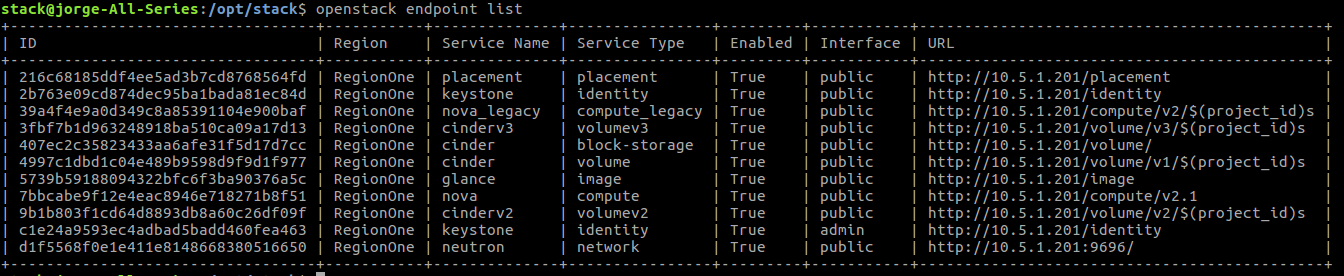
\includegraphics[width=1\textwidth]{imagenes/capitulo4/endpointlist.png}
    \caption{Lista de endpoints.}
	\vspace{0.3cm}
    \label{endpointlist}
\end{figure}

Pero aún así, esta forma de trabajo requiere trabajar con comandos complicados, motivo por el que existe Horizon. En la Fig.\ref{DashboardInicio} podemos ver el listado de los endpoints cliclando en "Acceso a la API" al acceder al escritorio o \textit{dashboard} de Horizon. Esta forma de trabajar es mucho más intuitiva al ser gráfica que el resto y será la preferida en algunos casos.


\begin{figure}
    \centering
    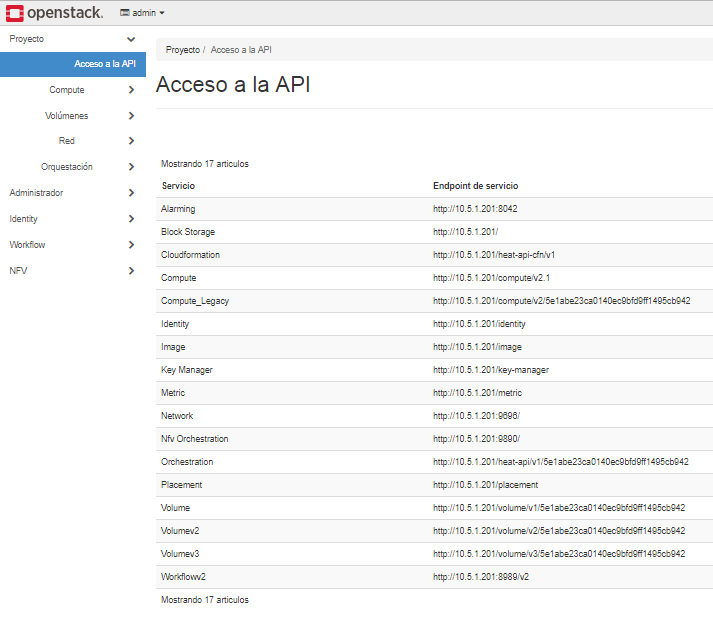
\includegraphics[width=1\textwidth]{imagenes/capitulo4/endpointlistHorizon.png}
    \caption{Lista de endpoints desde Horizon.}
	\vspace{0.3cm}
    \label{DashboardInicio}
\end{figure}

\section{Heat} \label{subchap:heat}

\begin{figure}
    \centering
    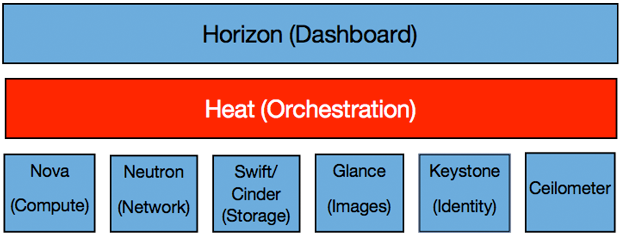
\includegraphics[width=0.7\textwidth]{imagenes/capitulo4/coordinacionHEat.png}
    \caption{Heat: capa de orquestación.}
	\vspace{0.3cm}
    \label{CapaHeat}
\end{figure}

En el capítulo \ref{chap:implementacion} donde vamos a ver como implementar nuestro entorno, veremos como utilizar el dashboard de Horizon y como trabajar desde la CLI. En los comienzos del cloud computing, aprovisionar de recursos mediante la línea de comandos pronto dejó de ser viable y los administradores comenzaron a realizar scripts en bash con la CLI para automatizar la creación de entornos. Pero pronto empezó a dar problemas este método. ¿Qué ocurre si ejecutamos un script accidentalmente, o si queremos eliminar sólo algunos recursos, o bien hacer un único cambio? Esta es la motivación del surgimiento de Heat. Además, esta evolución hacia Heat la veremos claramente tras leer el capítulo \ref{chap:implementacion} de implementación, en el que se verá la administración del entorno con estas herramientas.

Heat se introdujo en 2013 con la versión \textit{Grizzly} de OpenStack. Se basa en una pila o \textit{stack} que no es mas que una descripción de los parámetros de orquestación donde se indican todos los recursos de OpenStack a aprovisionar. Heat se ocupa por tanto del aprovisionamiento y la configuración sin necesidad de preocuparnos de las dependencias o el orden de ejecución, creando así una capa de abstracción entre los servicios básicos (Fig.\ref{CapaHeat}). Además, Heat es compatible con  el formato de plantillas de AWS CloudFormation.


\subsection{Arquitectura de Heat}
Hay cuatro componentes esenciales de un proyecto en Heat que podemos ver en la Fig.\ref{heat_architecture}, cada uno con una única función \cite{dorn_heat_2017}:
\begin{itemize}
\item \textbf{heat}. Es la CLI que se comunica con la API de heat, heat-api.
\item \textbf{heat-api}. Es el componente que proporciona una API REST nativa de OpenStack que procesa las solicitudes y las envía al motor heat-engine.
\item \textbf{heat-api-cfn}. Este componente proporciona una API de consulta del estilo AWS que es compatible con AWS CloudFormation y procesa las solicitudes y las envía a heat-engine.
\item \textbf{heat-engine}. Es el cerebro de la operación y hace el trabajo principal de orquestar el lanzamiento de plantillas o \textit{templates} y proporcionar respuesta al usuario de la API.
\end{itemize}

\begin{figure}
    \centering
    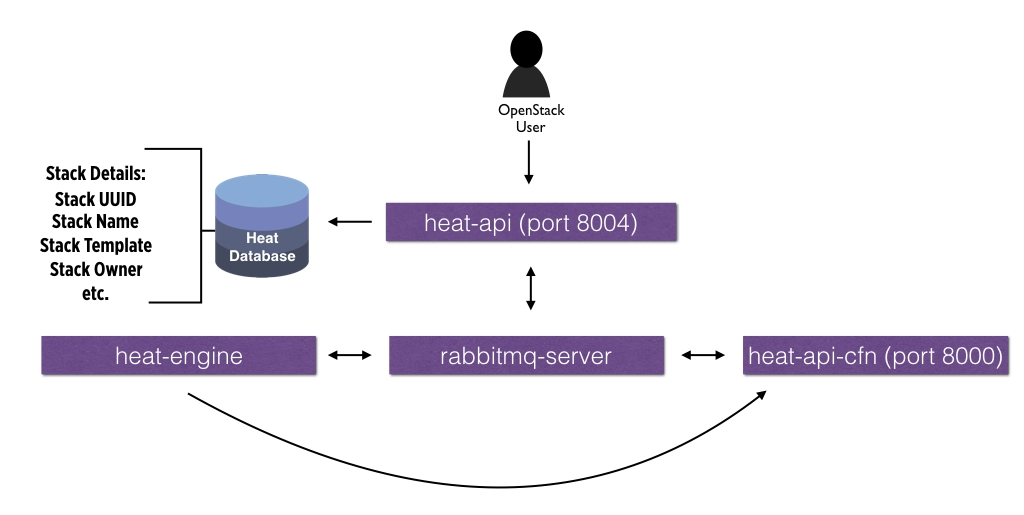
\includegraphics[width=0.7\textwidth]{imagenes/capitulo4/heat_architecture.png}
    \caption{Arquitectura de Heat.}
	\vspace{0.3cm}
    \footnotesize{Fuente: Matt Dorn, "Preparing for the Certified OpenStack Administrator Exam" Packt Publishing, 2017 }
    \label{heat_architecture}
\end{figure}


\subsection{Conceptos sobre Heat}

Ahora que conocemos los componentes de Heat vamos a presentar una serie de conceptos más sobre esta herramienta de orquestación:

\begin{itemize}
\item \textbf{Resources}. Son objetos que se crearán o modificarán durante la orquestación. Los recursos pueden ser redes, routers, subredes, instancias, volúmenes, direcciones IP flotantes, grupos de seguridad y más.
\item \textbf{Stack}. En Heat, una pila o stack es una colección de recursos.
\item \textbf{Parameters}. Permiten al usuario proporcionar información a la plantilla durante la implementación. Por ejemplo, si desea ingresar el nombre de una instancia durante la orquestación, ese nombre podría ingresarse como un parámetro en la plantilla y cambiarse cada vez que se ejecute.
\item \textbf{Template}. Plantilla en la que se indica como se define y describe un stack con código.
\item \textbf{Output}. Como su nombre indica, las salidas proporcionan información al usuario.
\end{itemize}

\subsection{Funcionamiento de Heat}
Ahora que entendemos los conceptos básicos sobre Heat, podemos comprender mejor cómo funciona.

\begin{enumerate}
\item La orquestación se define en un template al describir los objetos (recursos) en un formato legible y fácilmente entendible.
\item El usuario crea el stack que hará que la herramienta heat-cli apunte al archivo y a los parámetros de la plantilla.
\item La herramienta heat-cli se comunica con  heat-api.
\item El heat-api envía la solicitud al heat-engine.
\item El heat-engine procesa la solicitud comunicándose con las otras APIs de OpenStack y devuelve la salida al usuario.
\end{enumerate}

\subsection{Heat Orchestration Template}

\begin{figure}
    \centering
    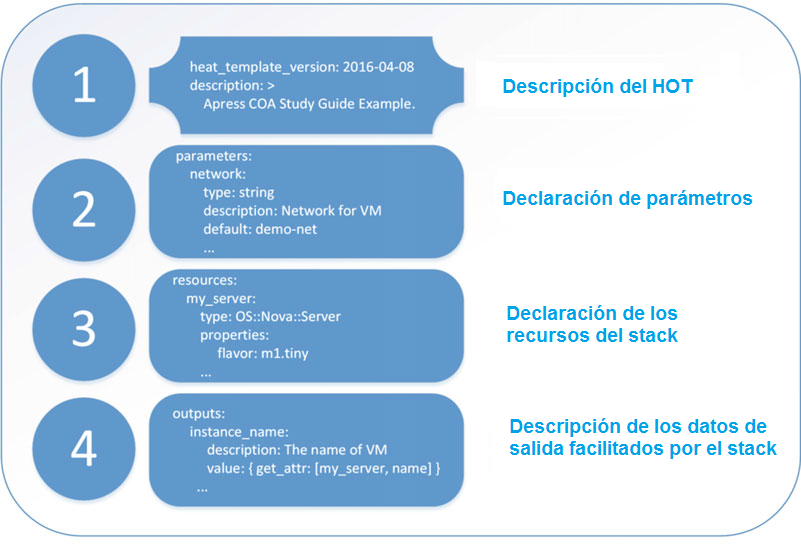
\includegraphics[width=0.7\textwidth]{imagenes/capitulo4/heat_template.png}
    \caption{Heat Orchestration Template.}
	\vspace{0.3cm}
    \footnotesize{Fuente: Andrey Markelov, “Certified OpenStack Administrator Study Guide”, apress, 2016 }
    \label{heat_template}
\end{figure}

Todos estos elementos aparecen al crear una plantilla como se aprecia en la Fig.\ref{heat_template} que muestra la anatomía de un template en Heat conocida como HOT (Heat Orchestration Template).

Una plantilla de Heat suele ser un archivo YAML, un lenguaje de serialización basado en JSON cuyo fin es su fácil comprensión y que contiene los siguientes campos \cite{dorn_horizon_2017}:

\begin{itemize}
\item Version.
\item Description.
\item Parameters.
\item Resources.
\item Output.
\end{itemize}

Sólo son obligatorios tres de los campos antes mencionados para obtener una plantilla básica: version, description y resources. 

%“” 
\section{Tacker}
Tacker es un proyecto oficial de OpenStack que construye un gestor genérico de VNF que se conoce como VNF Manager (VNFM) y un orquestador de NFV, NFV Orchestrator (NFVO), para implementar y operar con los servicios de red y las funciones de red virtual (VNF), en una plataforma que proporcione la infraestructura como OpenStack. 

Tacker se basa en ETSI MANO Architectural Framework \ref{arquitectura-NFV} para formar su arquitectura \ref{TackerArquitectura} y proporciona un stack funcional para la orquestación de servicios de red extremo a extremo utilizando VNFs.\cite{noauthor_tacker_nodate}

\begin{figure}
    \centering
    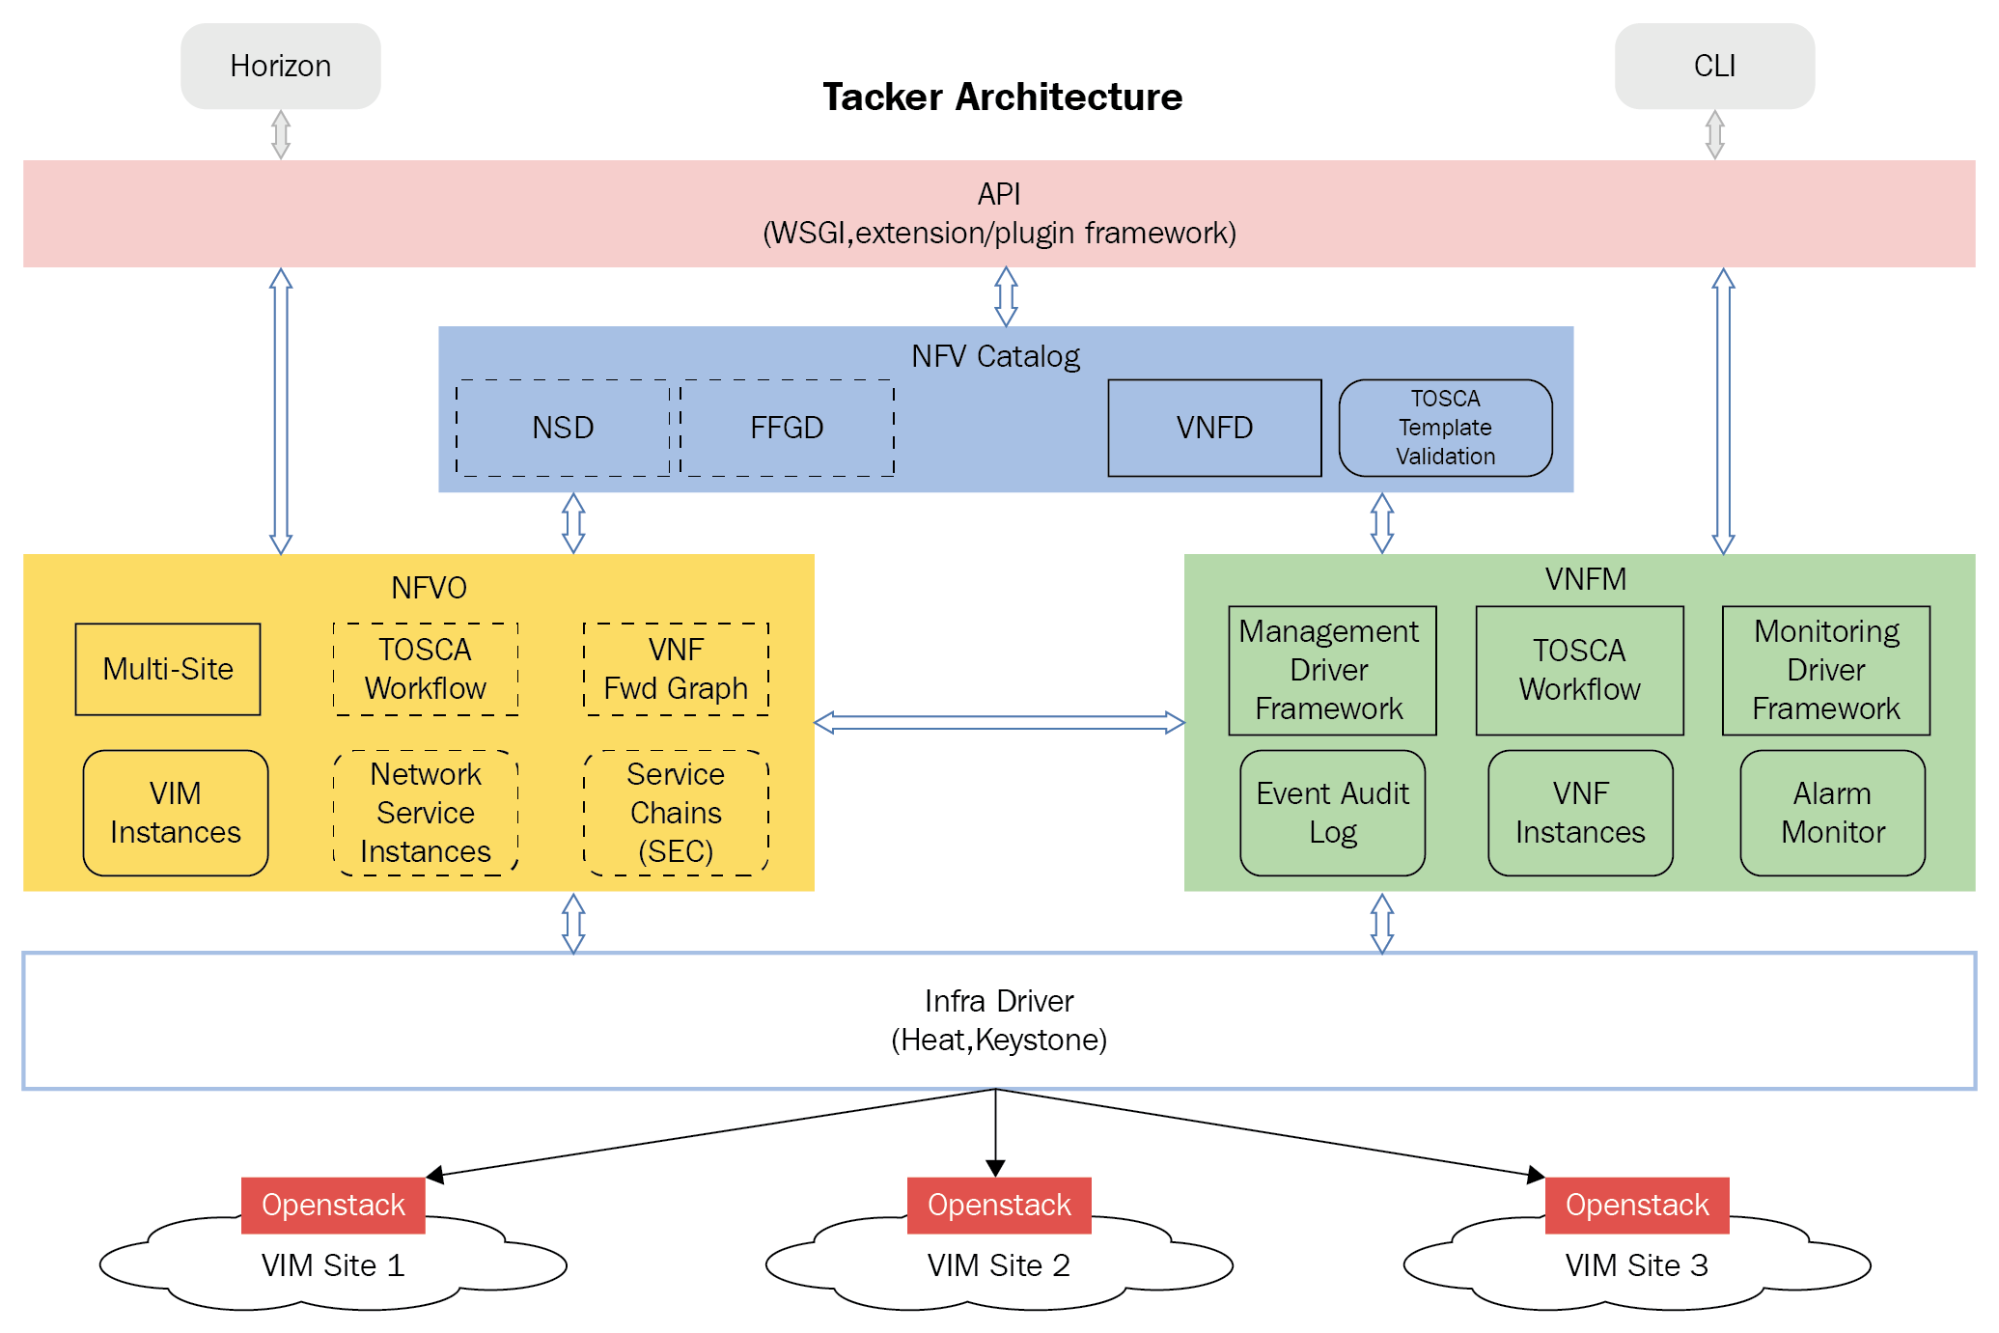
\includegraphics[width=0.7\textwidth]{imagenes/capitulo4/TackerArquitectura.png}
    \caption{Arquitectura de Tacker.}
	\vspace{0.3cm}
    \footnotesize{Fuente: Openstack Wiki}
    \label{TackerArquitectura}
\end{figure}

\begin{tcolorbox}[colback=orange!5!white,colframe=orange!75!black]
Jorge: Entiendo que lo siguiente aún no está hecho, porque habría que poner algún texto introductorio...
\end{tcolorbox}


\subsection{Motivación de Tacker}
En la mayoría de las demandas en telecomunicaciones, la alta disponibilidad y fiabilidad en su infraestructura es crítica. 

Al igual que la mayoría de las plataformas cloud y aplicaciones nativas en la nube, esto se logra a través de la escalabilidad horizontal de la arquitectura a consta de dejar a un lado las prácticas tradicionales de escalabilidad vertical en las que únicamente se requiere cada vez de más hardware y mayor capacidad. 

A pesar de no poder asegurar proporcionar el 99.999\% del tiempo de actividad del hardware en un entorno cloud, si podemos crear mecanismos que hagan que los servidores trabajen como un clúster con la finalidad de repartir el trabajo y asegurar alta disponibilidad. 

De esto trata la escalabilidad horizontal, cuya naturaleza es distribuida. Más allá de desplegar una infraestructura celular usando distintos nodos de Nova en OpenStack, Tacker ayuda a aumentar la disponibilidad. 

\subsection{Funciones de Tacker}
Dentro de los recursos y funciones de red virtual extremo a extremo que proporciona encontramos: 

\subsubsection{Catálogo NFV:} 
\begin{itemize}
\item VNF Descriptors, (VNFD).
\item Network Services Descriptors, (NSD).
\item VNF Forwarding Graph Descriptors, (VNFFGD).
\end{itemize}

Todos estos descriptores se basan OASIS TOSCA \cite{noauthor_tosca_nodate} y proporcionan algunos requisitos para definir descriptores de servicio de red (NSD), descriptores VNF (VNFD) y descriptores de gráficos de reenvío VNF (VNFFGD) utilizando \textit{TOSCA templates}. Estas plantillas se analizan y se traducen en plantillas de Heat, transmitiéndose después a un controlador que interactúa con la infraestructura de OpenStack, Heat y Keystone. La relación de estos descriptores con la arquitectura de Tacker podemos verla en la Fig.\ref{TackerArquitecturaDescriptores}.

\begin{figure}
    \centering
    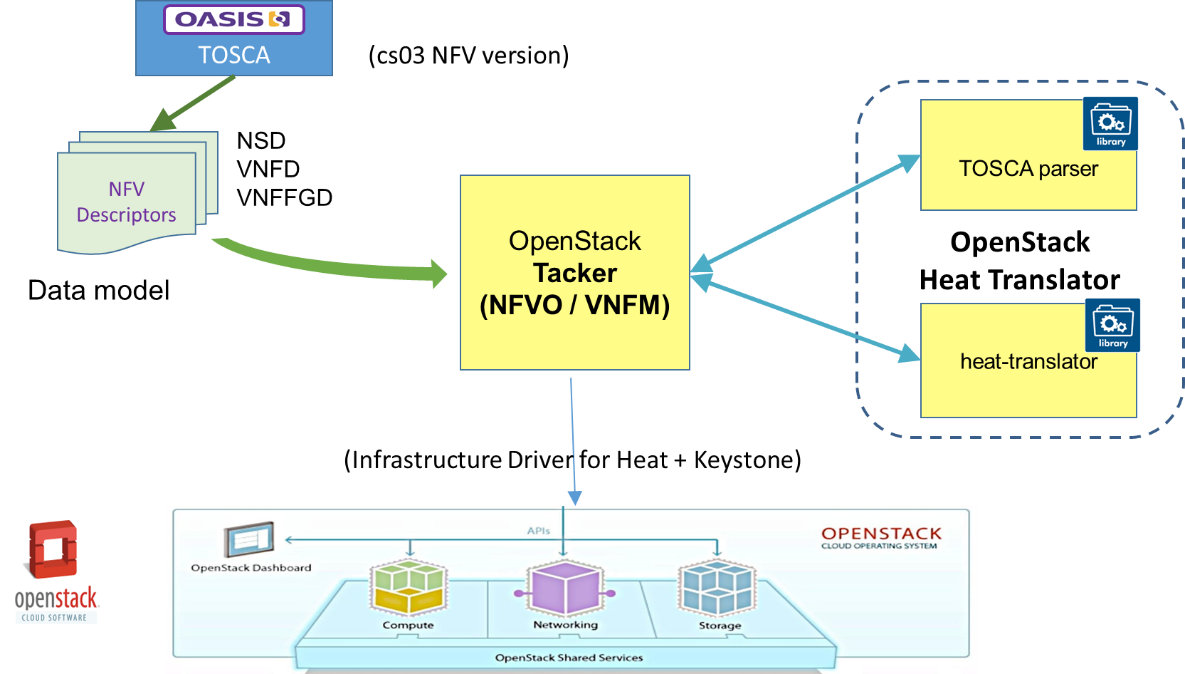
\includegraphics[width=0.7\textwidth]{imagenes/capitulo4/DescriptoresTacker.png}
    \caption{Descriptores en arquitectura de Tacker.}
	\vspace{0.3cm}
    \footnotesize{Fuente: Openstack Wiki}
    \label{TackerArquitecturaDescriptores}
\end{figure}

\subsubsection{VNFM:} 
\begin{itemize}
\item Ciclo de vida básico de una VNF (crear / actualizar / eliminar).
\item Posicionamiento mejorado basado en plataforma (EPA) de cargas de trabajo NFV de alto rendimiento.
\item Supervisión del estado de las VNFs implementadas.
\item Auto-recupearción / auto-escalado  de VNFs basado en políticas.
\item Facilitar la configuración inicial de cada VNF.
\end{itemize}

\subsubsection{NFVO:} 
\begin{itemize}
\item Implementación de servicios de red  extremo a extremo mediante el uso de plantillas que incorporan VNFs.
\item Políticas de despliegue de VNF para garantizar su formación de manera eficiente.
\item Conexión de VNFs mediante SFC (\textit{Service Function Chaining}),  especificadas en un descriptor VNF Forwarding Graph Descriptor.
\item Verificaciones de recursos VIM y asignación de recursos.
\item Capacidad de organizar VNFs en múltiples VIM y regiones múltiples (POPs).
\end{itemize}

\section{Ceilometer}
Dentro de los servicios de telemetría que ofrece OpenStack encontramos \textit{Ceilometer}. El proyecto Ceilometer es un servicio de recopilación de datos de medición y eventos de los servicios de OpenStack. Estos datos pueden ser utilizados por otros proyectos de OpenStack para actuar en función de ellos como en el caso de Heat y son almancenados en una base de datos \textit{MongoDB}.

El servicio de telemetría consta de los siguientes componentes \cite{noauthor_celiometer_nodate}:

\begin{itemize}
\item \textbf{Compute agent (ceilometer-agent-compute)}. Se ejecuta en cada nodo de cómputo para sondeos y estadísticas de utilización de recursos.
\item \textbf{Central agent (ceilometer-agent-central)}. Se ejecuta en un servidor de administración central para sondear las estadísticas de utilización de recursos no vinculados a instancias o nodos de cómputo. Se pueden iniciar múltiples agentes para escalar el servicio horizontalmente. 
\item\textbf{Notification agent (ceilometer-agent-notification)}. Se ejecuta en un servidor central de administración y consume mensajes de la o las colas de mensajes para generar datos de eventos y medición. Los datos se entregan a los destinatarios pertinentes.
\end{itemize}





\chapter{Diseño} \label{chap:diseno}
El objetivo de este apartado será explicar el diseño por el que se ha optado tanto físico como lógico y los motivos que han hecho que tomemos esas decisiones. 

\section{Diseño físico del entorno}

Para el dimensionado del entorno físico, se ha tenido en primer lugar en cuenta el objetivo del proyecto. Dado que la motivación del mismo es crear una infraestructura en la que podríamos implementar cualquier servicio y dotarla de mecanismos de orquestación de funciones de red que proporcionen escalabilidad y redundancia para asegurar alta disponibilidad, en principio se pensó el instalar cuatro máquinas distintas: dos en una localización geográfica y otras dos en otra diferente. En cada una de las localizaciones tendríamos un servidor dedicado con los servicios de autenticación (Keystone) y dashboard (Horizon), que compartirían los datos de todos los usuarios y proyectos disponibles, y en los otros dos el resto de servicios de OpenStack. Además cada localización tendría una IP pública de acceso distinta, creando así un entorno multi-región como el que aparece en la Fig.\ref{active-active-region}

Puesto que sólo pudimos disponer de dos equipos y una dirección IP pública, para la configuración de la infraestructura física hemos optado por realizar la configuración de la Fig.\ref{fisico}, donde tenemos dos servidores interconectados entre sí, cada uno de ellos simulando una localización geográfica distinta.

El acceso al exterior se hará a través del Servidor 1 para ambas configuraciones de OpenStack que es el que tiene una toma que conecta con el ISP que nos da acceso a la red pública con IP 150.214.190.177. Además se instaló una tarjeta de red en el Servidor 1 para poder conectarlo al Servidor 2 a través de la red 10.5.2.0/24 y que este pueda salir a través del Servidor 1 hacia Internet, creando así el direccionamiento que podemos apreciar en el esquema anterior.

Por último, mencionar que los servidores se instalarán en el despacho 2.21 de la ETSIIT.

\begin{figure}
    \centering
    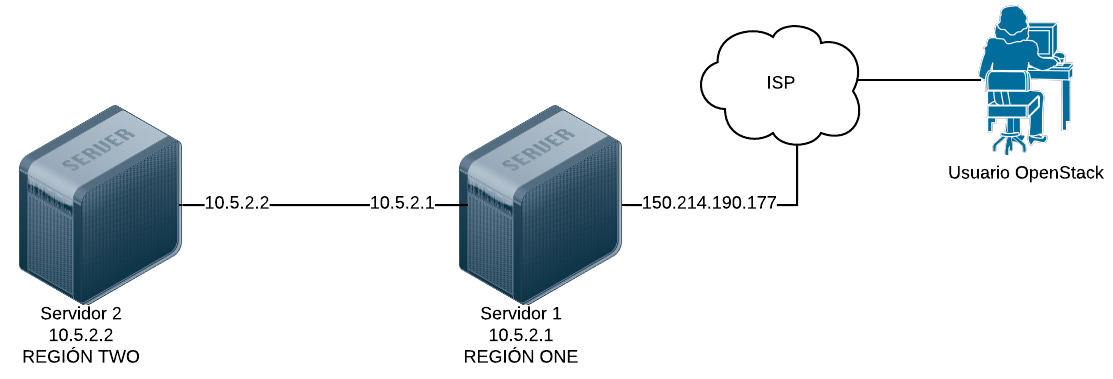
\includegraphics[width=0.7\textwidth]{imagenes/capitulo5/fisico.png}
    \caption{Diseño físico de la infraestructura.}
	\vspace{0.3cm}
    \label{fisico}
\end{figure}

\section{Diseño de un entorno multi-región}

El objetivo de este diseño multi-región, es el de poder usar de forma activa más de una localización geográfica en nuestra cloud proporcionando redundancia, orquestación  y alta disponibilidad, de forma que conseguimos una administración centralizada de nuestra nube, pudiendo disponer de la recuperación de los servicios que se quisieran implementar en la nube ante posibles desastres. 

Si nos fijamos en la Fig.\ref{fisico}, veremos que la Región One, será la implementación de OpenStack con todos sus servicios en el Servidor 1, mientras que la Región Two, será la implementación de OpenStack con todos los servicios que instalemos salvo Keystone y Horizon, pues estos servicios se gestionarán desde el Servidor 1.

Los componentes de la arquitectura por tanto son:

\begin{itemize}
\item Dos implementaciones separadas de OpenStack en la nube, que a su vez equivalen a dos regiones. En este ejemplo, tenemos la Región One y la Región Two \ref{active-active-region}. Estas regiones ejecutan los servicios principales de OpenStack, excepto Keystone y Horizon. Cada región puede tener todos los AZ nodos complementarios que se deseen, aunque en nuestro caso se pondrá un único nodo en cada una.
\item Otra región OpenStack dedicada exclusivamente a hospedar los servicios Keystone y Horizon. Esta región podría clasificarse como la región de administración. En el despliegue que haremos, debido a que sólo disponemos de dos servidores, los servicios de Keystone y Horizon se desplegarán en uno de los servidores, el Servidor 1, que equivale en la Fig.\ref{active-active-region} a la Región One.
\item Las regiones One y Two aprovechan la región de administración para gestionar la autenticación y la interfaz web de la GUI al centralizar la gestión y creación de usuarios, inquilinos y proyectos, proporcionando un solo dashboard para administrar todas las regiones activas.
\end{itemize}


Debida a las limitaciones presentadas, en la sección \ref{subsec:DespliegueProduccion}, se propone el despliegue de un entorno en producción donde se pueda disponer de más nodos.

\begin{figure}
    \centering
    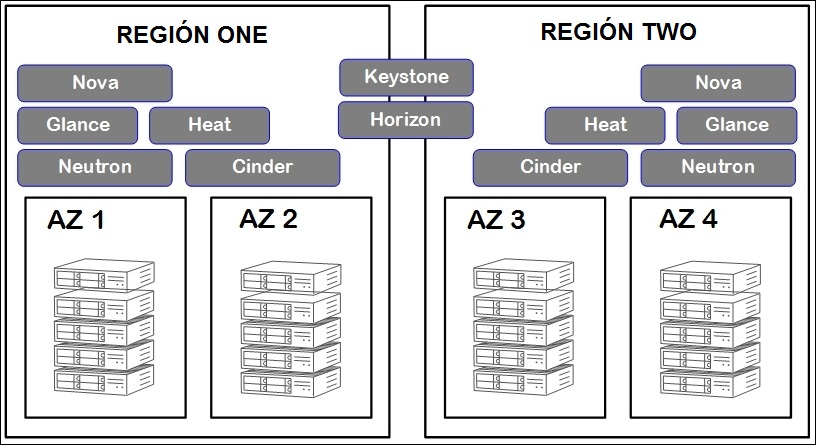
\includegraphics[width=0.7\textwidth]{imagenes/capitulo5/active-active-region.png}
    \caption{Entorno Multi-Región.}
	\vspace{0.3cm}
    \footnotesize{Fuente: Walter Bentley, "OpenStack Administration with Ansible 2 - Second Edition" Packt Publishing, 2016 }
    \label{active-active-region}
\end{figure}

\section{Diseño lógico}
Una vez hayamos conseguido implementar esta configuración los objetivos de diseño serán varios, resultando el esquema de la Fig.\ref{logicoSDN}:

\begin{figure}
    \centering
    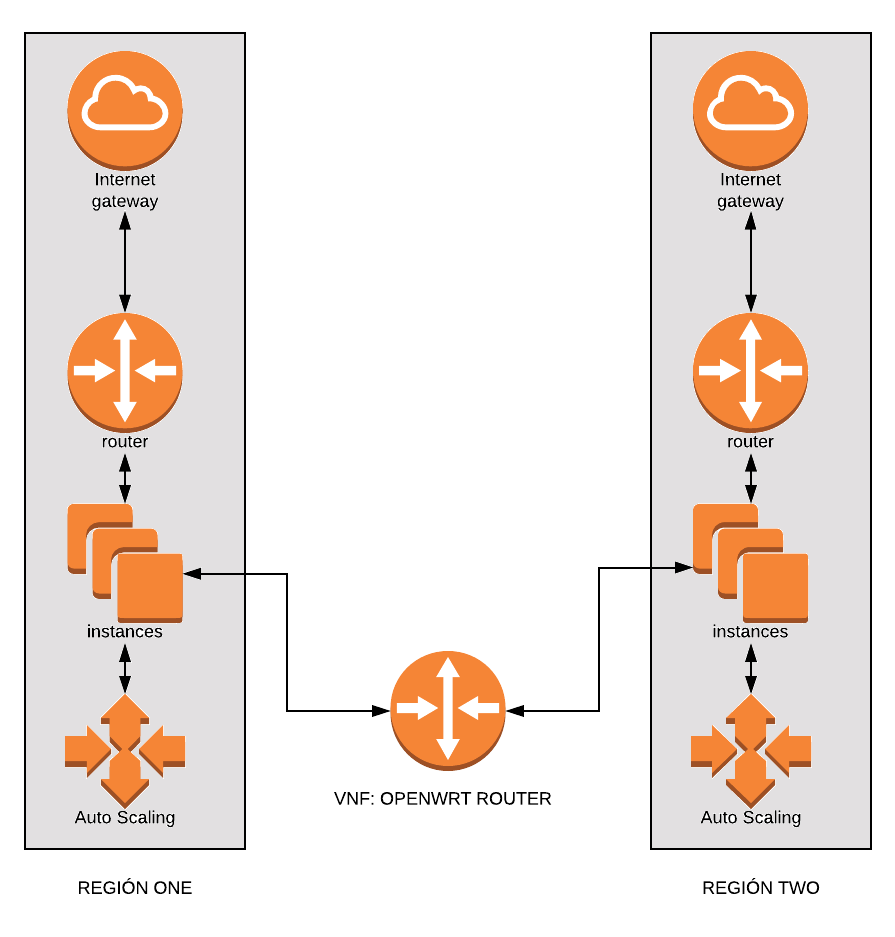
\includegraphics[width=0.7\textwidth]{imagenes/capitulo5/logico.png}
    \caption{Diseño del escenario de red a crear con OpenStack.}
	\vspace{0.3cm}
    \label{logicoSDN}
\end{figure}

\begin{tcolorbox}[colback=red!5!white,colframe=red!75!black]
En este esquema se puede poner también floating IP, y diferenciar entre las distintas capas y la red interna y externa.
\end{tcolorbox}

\begin{itemize}
\item Configurar un esquema de red SDN, basado en un esquema de red jerárquico por capas conforme a lo aprendido durante el Grado en la especialidad de Telemática. En el tendremos la capa de acceso, donde implementaremos las instancia, y la capa de distribución con core colapsado que estará formada por los routers SDN que nos darán acceso a la red externa.
\item Este esquema de red se creará en primer lugar en la Región One, a través del dashboard de Horizon.
\item En la Región Two, implementaremos un esquema de red similar pero esta vez gestionado desde la CLI.
\item Usaremos Heat para la orquestación de distintas instancias de forma automática en base al uso de la CPU de las mismas. De este modo estaremos haciendo gestión de NFVs y autoescalado con el uso de HOT.
\item Por último, crearemos una VNF que en este caso será un router OpenWRT, para interconectar instancias de ambas regiones con el uso de Tacker, realizando así la orquestación de esta NFV en concreto.
\end{itemize}

\subsection{Requisitos del diseño lógico}
Para llevar a cabo este diseño, necesitaremos crear algunos recursos:

\begin{itemize}
\item Creación del entorno SDN. Se crearán los routers, redes y subredes necesarios para la implementación de los escenarios tal y como se verá en el siguiente capítulo.
\item Floating IP. Lo ideal para crear IPs flotantes sería disponer de varias IPs públicas, dado que no es el caso, en ambos servidores se crearán interfaces virtuales en las tarjetas de red para poder abordar el problema de disponer de una sola IP pública. El concepto de  IP flotante se verá con detalle en la sección \ref{subsec:IP-flotante} del siguiente capítulo.
\item Listas de acceso / Firewall. Debemos de establecer listas de acceso que actuarán de firewall para declarar el tráfico tanto entrante como saliente que deseamos permitir. En Openstack esto se hace a través de los \textit{security groups}. Crearemos reglas par permitir cualquier tráfico saliente y sólo el tráfico IP, SSH, y HTTP entrante.
\item Instancias. Las instancias se preparan para ser capaces de alojar cualquier servicio que quisiéramos dar.
\item Key Pair. También necesitaremos crear un par de claves público-privadas para acceder a las instancias de forma segura.
\item Imágenes. La forma más sencilla de obtener una imagen de una máquina virtual que funcione con OpenStack es descargar una ya creada. En este caso será Cirros como veremos más adelante, debido a su pequeño tamaño.
\item Almacenamiento. Por defecto, las instancias que creemos no tendrán espacio para el almacenamiento. Con el servicio de Cinder conseguiremos proveer de almacenamiento persistente a las imágenes.
\item HOT. Plantilla de Heat donde definiremos los parámetros necesarios para la orquestación de NFVs de forma que consigamos crear o borrar instancias en función del uso de la CPU de las mismas.
\item TOSCA Template. Plantilla que contendrá el código necesario para crear una VNF que implemente un router OpenWRT que permita interconectar ambas regiones mediante NFV.
\end{itemize}









\chapter{Implementación} \label{chap:implementacion}
\begin{tcolorbox}[colback=red!5!white,colframe=red!75!black]
AQUÍ HABLAR DE CONCEPTOS RELACIONADOS CON LA CARRERA: DISEÑO JERÁRQUICO, =! CAPAS, LISTAS DE ACCESO..
\end{tcolorbox}

Nos basaremos en la versión\textit{ Queens }de OpenStack que es la versión estable más actualizada hasta la fecha \cite{noauthor_releases:_nodate}.

\section{Desplegando OpenStack}
En este punto vamos a ver las opciones que tenemos para implementar nuestra nube IaaS con OpenStack y como lo haremos finalmente con el uso de una todo en uno (\textit{all-in-one}). Eso significa que  los diferentes servicios de OpenStack se ejecutarán en la misma máquina, que puede ser una máquina física o una máquina virtual y servirá de guía para implementar OpenStack en Ubuntu.

\subsection{Métodos de despliegue}\label{subsesc:metodosdespliegue}
OpenStack se puede implementar de varias maneras:

\begin{itemize}
\item Manualmente. OpenStack se puede implementar manualmente mediante la aplicación de los pasos descritos en la documentación pertinente \cite{noauthor_install_nodate}.
\item Scripted. También se puede implementar de forma guiada mediante el uso de una solución como Packstack o DevStack, que será la que nosotros usemos.
\item Despliegue a gran escala. Otra opción es el despliegue de OpenStack a gran escala, utilizando soluciones de implementación más avanzadas, como Triple O, Director \cite{noauthor_tripleo_nodate}\cite{noauthor_director_nodate}.
\end{itemize}

\subsection{El rol de los tipos de nodo}\label{subchap:rol-nodos}
Normalmente, existen diferentes roles según el tipo de nodo en una nube de OpenStack como vemos en la Fig.\ref{nodos} Los roles que se utilizan dependen de la configuración existente:

\begin{figure}
    \centering
    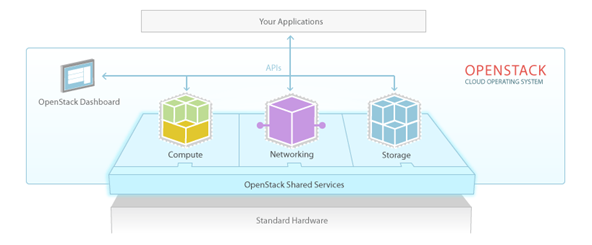
\includegraphics[width=0.7\textwidth]{imagenes/capitulo6/nodos.png}
    \caption{Tipos de nodos en OpenStack.}
	\vspace{0.3cm}
    \footnotesize{Fuente: OpenStack wiki}
    \label{nodos}
\end{figure}

\begin{itemize}
\item Nodo controlador (\textit{Controller node}). Ejecuta los servicios de control. En este nodo encontraremos servicios como Keystone , la cola de mensajes, la base de datos MariaDB y todo lo esencial para controlar la nube.
\end{itemize}

\begin{itemize}
\item Nodo controlador de red (\textit{Network controller node}).  Proporciona servicios de red a la nube. Es el tipo de no que proporciona SDN y está conectado a redes internas y externas.
\end{itemize}

\begin{itemize}
\item Nodo de cómputo (\textit{Compute nodes}). Son los nodos que realmente van a ejecutar las instancias en OpenStack. Básicamente, los compute nodes son los hipervisores y en ellos algunas partes de Nova se están ejecutando para interactuar con el hipervisor, lo que permite a OpenStack programar el funcionamiento de máquinas virtuales en un nodo de cómputo específico.
\end{itemize}

\begin{itemize}
\item Nodos de almacenamiento (\textit{Storage nodes}). Los nodos de almacenamiento son todo lo que involucra  el almacenamiento de objetos (servicios como Swift o Ceph) y en un clúster de almacenamiento avanzado, estamos hablando fácilmente de docenas de storage nodes para garantizar la disponibilidad del mismo.
\end{itemize}

Aunque hagamos referencia a un nodo, en un entorno en producción redundante podrá haber tantos como sean necesarios de cada tipo para asegurar alta disponibilidad. 

\subsection{Despliegues con Devstack}
\textit{DevStack} es la solución estándar para la creación de un entorno de pruebas con OpenStack y se ejecuta en múltiples distribuciones de Linux incluyendo Ubuntu, Fedora, OpenSUSE, Debian, CentOS o RedHat entre otras. DevStack proporciona una serie de scripts para montar un entorno OpenStack completo basado en la configuración que especificaremos en un archivo destinado a ese fin. 

DevStack es muy popular entre los desarrolladores, ya que se usa para pruebas de desarrollo y operativas. Es importante señalar que DevStack no se creó para su uso en producción.

Se pueden usar diferentes escenarios al configurar un entorno de laboratorio basado en Ubuntu con DevStack:

\begin{itemize}
\item All-in-one Single VM.
\end{itemize}

\begin{itemize}
\item All-in-one Single Machine.
\end{itemize}

\begin{itemize}
\item Multi-node Lab.
\end{itemize}

La dos primeras son la instalación todo en uno con la salvedad de realizarla en un máquina virtual o una máquina física. La última, puede usar varias VMs o máquinas físicas. 

Optaremos por la segunda opción para realizar la implementación de este proyecto por motivos obvios de disponibilidad de equipos y presupuesto, es decir, una configuración all-in-one en una máquina física, lo cual significa que no haremos una distinción estricta entre los tipos de nodos vistos sino que tendremos una máquina en el entorno creado que proporcione las funciones de todos estos nodos.

\section{Proceso de instalación}
Usaremos Ubuntu Server 16.04.3 LTS como sistema operativo. Para ello, el departamento de Telemática cedió dos servidores dedicados ya que en el proceso de instalación se hacen cambios sustanciales en la configuración del equipo y además se requiere de altos requisitos hardware para que el funcionamiento del despliegue sea óptimo.

Vamos a comenzar con la implementación de OpenStack mediante Devstack . El proceso de instalación será similar en ambos servidores con algunas salvedades.

\subsection{Puesta a punto de los servidores}
En primer lugar, una vez instalado en ambos servidores el sistema operativo, haremos una serie de verificaciones. 

Para empezar, necesitamos verificar la memoria RAM disponible, ya que si no tenemos 8 GB como mínimo, la instalación fallará. Inicialmente teníamos 16 GB en el primer servidor y tras la instalación:

\begin{lstlisting}[style=Consola]
jorge@wimunet4::~$ free
         total     used     free   shared  buff/cache  available
Mem:  16298968   5222208  8664664    9464     2412096   10721112
Swap:  2097148        0  2097148
\end{lstlisting}

Y 32 GB en el segundo servidor por lo que esta parte queda cubierta:

\begin{lstlisting}[style=Consola]
jorge@wimunet5:~$ free
         total     used      free   shared  buff/cache  available
Mem:  32610848  1025700  26423112   361292     5162036   30669864
Swap: 33221628        0  33221628
\end{lstlisting}

Puesto que los servidores están dentro de la ETSIIT, tras solicitar una IP pública se nos asignó la 150.214.190.177. Una vez obtenida configuramos el Servidor 1 modificando el archivo /etc/network/interfaces de nuestra máquina como sigue:

\begin{lstlisting}[style=Consola]
jorge@wimunet4::~$ cat /etc/network/interfaces
# interfaces(5) file used by ifup(8) and ifdown(8)
auto lo
iface lo inet loopback
	
auto enp3s0
iface enp3s0 inet static
	address 150.214.190.177
	netmask 255.255.254.0
	gateway 150.214.190.222
	dns-nameservers 150.214.204.10

auto enp3s0:1
iface enp3s0:1 inet static
	address 10.5.1.201
	netmask 255.255.255.0
\end{lstlisting}

De este modo conseguimos:
\begin{itemize}
\item Acceso a Internet con la IP pública 150.214.190.177.
\item Creación de la interfaz virtual \textit{enp3s0:1} que nos permitirá asignar a las instancias que creemos IPs flotantes (ver sección \ref{subsec:IP-flotante}) dentro de la red 10.5.1.201/24 para su acceso desde el exterior resolviendo así la problemática de tener una única IP pública.
\end{itemize}

De forma análoga modificamos las interfaces del Servidor 2 para acceder al exterior a través del Servidor 1 y tener también la posibilidad de asignar IPs flotantes en la red 10.5.3.201/24 creando la interfaz \textit{enp0s31f6:2}:

\begin{lstlisting}[style=Consola]
iface enp0s31f6 inet static
        address 10.5.2.2
        netmask 255.255.255.0
        gateway 10.5.2.1
        dns-nameservers 150.214.204.10
        dns-search ugr.es

auto enp0s31f6:2
iface enp0s31f6:2 inet static
        address 10.5.3.201
        netmask 255.255.255.0
\end{lstlisting}

Como comentamos en el capítulo anterior, para conectar ambos servidores se instaló una tarjeta de red en el Servidor 1 para comunicar ambos servidores a través de la red 10.5.2.0/24. 

Así en el Servidor 1 disponemos de una interfaz nueva con la IP 10.5.2.1:

\begin{lstlisting}[style=Consola]
jorge@wimunet4:~$ ifconfig enx6038e0e3083f
enx6038e0e3083f Link encap:Ethernet  HWaddr 60:38:e0:e3:08:3f
          inet addr:10.5.2.1  Bcast:10.5.2.255  Mask:255.255.255.0
          inet6 addr: fe80::6238:e0ff:fee3:83f/64 Scope:Link
          UP BROADCAST RUNNING MULTICAST  MTU:1500  Metric:1
          RX packets:1134037 errors:0 dropped:0 overruns:0 frame:0
          TX packets:1747042 errors:0 dropped:0 overruns:0 carrier:0
          collisions:0 txqueuelen:1000
          RX bytes:89409470 (89.4 MB)  TX bytes:2337586769 (2.3 GB)
\end{lstlisting}

Y en el Servidor 2, asignamos a la tarjeta de red la IP 10.5.2.2:

\begin{lstlisting}[style=Consola]
jorge@wimunet5:~$ ifconfig enp0s31f6
enp0s31f6 Link encap:Ethernet  HWaddr 2c:fd:a1:6e:c3:cf
          inet addr:10.5.2.2  Bcast:10.5.2.255  Mask:255.255.255.0
          inet6 addr: fe80::2efd:a1ff:fe6e:c3cf/64 Scope:Link
          UP BROADCAST RUNNING MULTICAST  MTU:1500  Metric:1
          RX packets:721537 errors:0 dropped:0 overruns:0 frame:0
          TX packets:490297 errors:0 dropped:0 overruns:0 carrier:0
          collisions:0 txqueuelen:1000
          RX bytes:929277285 (929.2 MB)  TX bytes:51982744 (51.9 MB)
          Interrupt:20 Memory:92f00000-92f20000
\end{lstlisting}

\subsection{Verificaciones sobre la configuración de los servidores}
Una vez preparados ambos servidores queda realizar algunas pruebas de conexión:

\begin{itemize}
\item Conectividad entre ambos servidores:
\end{itemize}
\begin{lstlisting}[style=Consola]
jorge@wimunet4:~$ ping 10.5.2.2
PING 10.5.2.2 (10.5.2.2) 56(84) bytes of data.
64 bytes from 10.5.2.2: icmp_seq=1 ttl=64 time=0.250 ms
64 bytes from 10.5.2.2: icmp_seq=2 ttl=64 time=0.201 ms
^C
--- 10.5.2.2 ping statistics ---
2 packets transmitted, 2 received, 0% packet loss, time 999ms
rtt min/avg/max/mdev = 0.201/0.225/0.250/0.028 ms

\end{lstlisting}

\begin{itemize}
\item Conexión del Servidor 1 a la red pública:
\end{itemize}
\begin{lstlisting}[style=Consola]
jorge@wimunet4:~$ ping www.google.es
PING www.google.es (216.58.201.163) 56(84) bytes of data.
64 bytes from mad08s06-in-f3.1e100.net (216.58.201.163): icmp_seq=1 ttl=54 time=12.2 ms
64 bytes from mad08s06-in-f3.1e100.net (216.58.201.163): icmp_seq=2 ttl=54 time=12.2 ms
^C
--- www.google.es ping statistics ---
2 packets transmitted, 2 received, 0% packet loss, time 1001ms
rtt min/avg/max/mdev = 12.239/12.251/12.264/0.111 ms

\end{lstlisting}

\begin{itemize}
\item Conexión del Servidor 2 a la red pública:
\end{itemize}
\begin{lstlisting}[style=Consola]
jorge@wimunet5:~$ ping www.google.es
PING www.google.es (172.217.16.227) 56(84) bytes of data.
64 bytes from mad08s04-in-f3.1e100.net (172.217.16.227): icmp_seq=1 ttl=53 time=13.1 ms
64 bytes from mad08s04-in-f3.1e100.net (172.217.16.227): icmp_seq=2 ttl=53 time=13.0 ms
^C
--- www.google.es ping statistics ---
2 packets transmitted, 2 received, 0% packet loss, time 1001ms
rtt min/avg/max/mdev = 13.052/13.096/13.141/0.122 ms
jorge@wimunet5:~$
\end{lstlisting}

Para que esta última conexión sea posible, en el Servidor 1 creamos un script en bash llamado \textit{network\_to\_second\_pc.sh} para permitir la conexión del Servidor 2 hacia Internet a través del Servidor 1 que es el que está conectado a la toma de la red externa.

\begin{lstlisting}[style=Consola]
jorge@wimunet4:~$ cat network_to_second_pc.sh
ifconfig enx6038e0e3083f 10.5.2.1/24
iptables -t nat -A POSTROUTING -o br-ex -j MASQUERADE
\end{lstlisting}

Como vemos, en él estamos creando una regla con el firewall \textit{iptables} para hacer \textit{postrouting} mediante NAT (\textit{Network Address Translation}) a través de la interfaz \textit{br-ex} que es la que nos da acceso en el Servidor 1 a la red pública.

\subsection{Instalando OpenStack}\label{sec:instalacion}
En este punto nos encontramos ya en disposición de instalar OpenStack. 

En primer lugar vamos a ver la parte que es idéntica para ambos servidores comenzando por la creación de un usuario con el nombre \textit{stack} y permisos de administrador:

\begin{lstlisting}[style=Consola]
jorge@wimunet4:~$  sudo useradd -s /bin/bash -d /opt/stack -m stack; echo "stack ALL=(ALL) NOPASSWD: ALL"| sudo tee /etc/sudoers.d/stack; sudo su - stack
\end{lstlisting}

A continuación, instalamos los paquetes \textit{cloud-init} que contienen un  conjunto de paquetes que son útiles cuando se trabaja con DevStack en una máquina Ubuntu. Básicamente son scripts de Python, Git y algunos más.

\begin{lstlisting}[style=Consola]
stack@wimunet4:~$ sudo apt-get install cloud-init
\end{lstlisting}

En esta parte de la configuración, pasamos a clonar todos los paquetes actuales de OpenStack  que están disponibles en Git \cite{noauthor_devstack:_2018} a la máquina local, con lo que conseguiremos poder comenzar con la instalación en la misma. Además indicamos que la versión que queremos instalar sea Queens.

\begin{lstlisting}[style=Consola]
stack@wimunet4:~$ git clone https://git.openstack.org/openstack-dev/devstack -b stable/queens
\end{lstlisting}

Tras esto, se habrá creado un directorio llamado \textit{devstack}:

\begin{lstlisting}[style=Consola]
stack@wimunet4:~$ cd devstack
\end{lstlisting}

Dentro de él existen distintos archivos, los que más nos interesarán son \textit{stack.sh, unstack.sh y clean.sh}, que se utilizan para instalar, desinstalar, y limpiar la configuración existente respectivamente. Necesitamos crear un archivo \textit{ local.conf}, al que antes hacíamos referencia y  que contendrá la configuración necesaria para que la instalación se realice acorde a nuestra necesidades. 

Este archivo será distinto para cada servidor. El archivo de configuración del Servidor 1 lo podemos ver en el apéndice \ref{sec:ConfServer1} y para el Servidor 2 en el \ref{sec:ConfServer2}.

Una vez creados ambos archivos podemos ya ejecutar el script \textit{stack.sh}, que leerá los parámetros de configuración de \textit{local.conf} y construirá nuestra IaaS multi-región con DevStack OpenStack basándose en estos parámetros.

\begin{lstlisting}
stack@wimunet4:~/devstack$ ./stack.sh
\end{lstlisting}

\begin{figure}
    \centering
    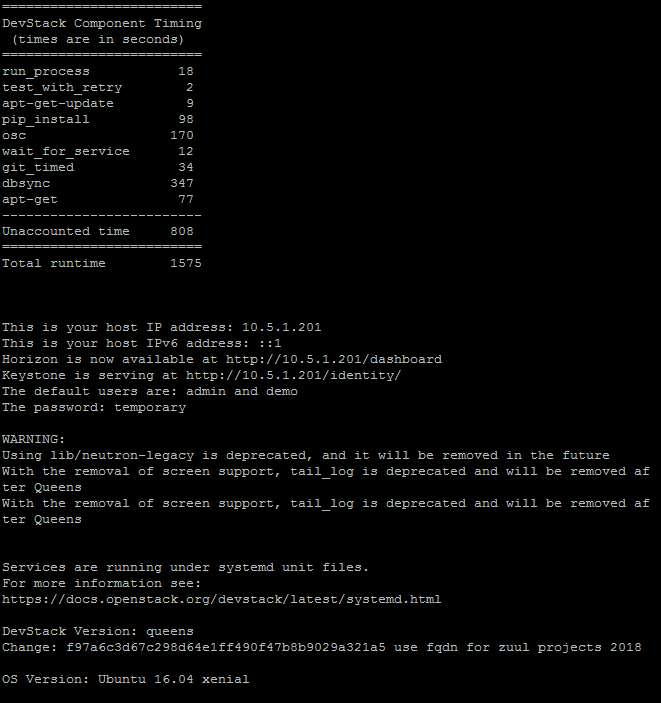
\includegraphics[width=1\textwidth]{imagenes/capitulo6/finInstalacionServer1.png}
    \caption{Reporte de la instalación.}
	\vspace{0.3cm}
    \label{fininstallserver1}
\end{figure}

El tiempo promedio de ejecución del script es largo y dependerá de la capacidad  del hardware de nuestro servidor. Cuando finaliza la instalación de manera correcta, nos mostrará un reporte de la misma, Fig.\ref{fininstallserver1}.
En el podemos ver el tiempo que ha demorado cada componente, nuestra dirección IPv4 e IPv6 y como se ha creado un usuario \textit{demo} que será un tenant además del usuario administrador, \textit{admin}. Por último, podemos ver que la versión instalada es \textit{Queens}, como ya hemos comentado, la versión estable más reciente que incorpora versiones actualizadas de los proyectos de OpenStack.\cite{noauthor_queens_nodate}

Después de implementar OpenStack en Ubuntu, abrimos un navegador en la dirección IP de la máquina donde  acabamos de alojar OpenStack, cuya IP pública es 150.214.190.177, en caso de que estemos accediendo a Horizon desde una red externa, mientras que desde el servidor podremos acceder directamente a la IP privada, 10.5.1.201 y conectarnos. Se mostrará entonces la página de la Fig.\ref{login} donde podremos iniciar sesión como admin utilizando la contraseña establecida. 

\begin{figure}
    \centering
    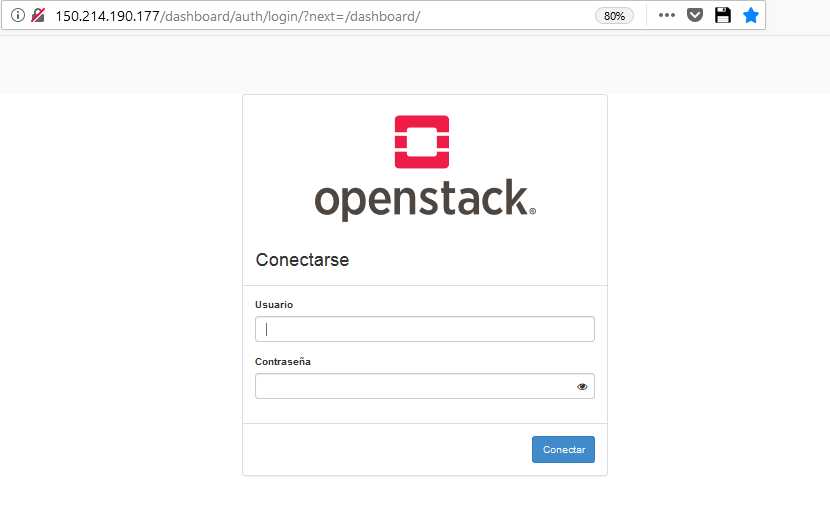
\includegraphics[width=1\textwidth]{imagenes/capitulo6/login.PNG}
    \caption{Página de acceso al dashboard de Horizon.}
	\vspace{0.3cm}
    \label{login}
\end{figure}

\section{Configuración de un escenario mediante Horizon}
Horizon es la herramienta más importante para los administradores que se están iniciando en OpenStack pues proporciona una interfaz web que facilita el trabajo como administrador de OpenStack.

\jorge{La figura 7.4 se ve muy poco, piensa si podrías ponerla en apaisado.}

\begin{figure}
    \centering
    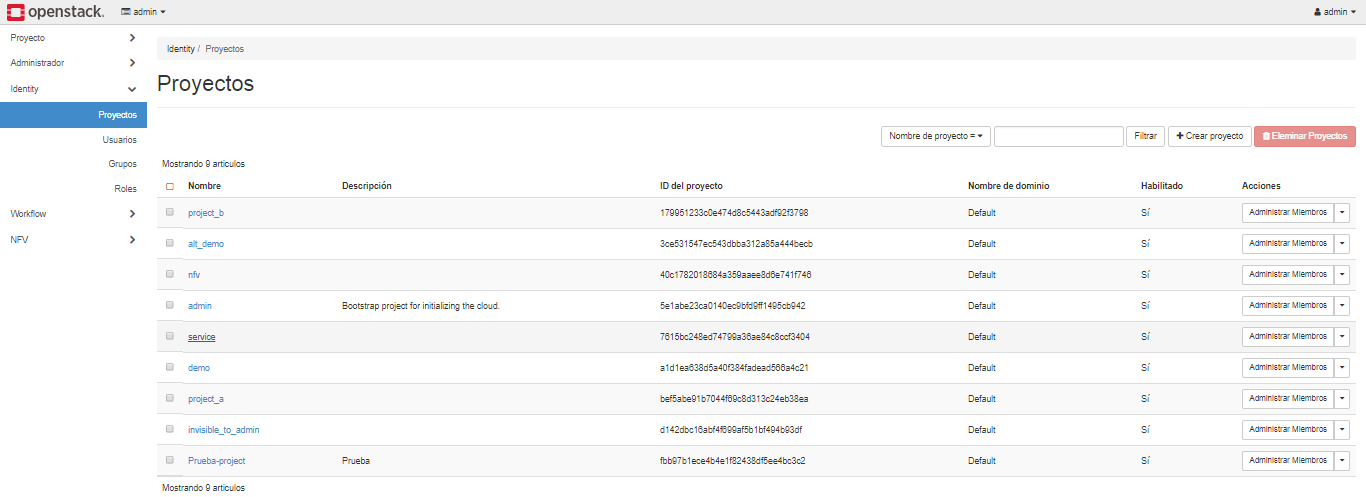
\includegraphics[width=1\textwidth]{imagenes/capitulo6/primeracceso.png}
    \caption{Panel inicial de Proyectos tras acceder a Horizon.}
	\vspace{0.3cm}
    \label{primeracceso}
\end{figure}

En este apartado procederemos con la implementación de instancias desde la interfaz web de Horizon. Trataremos el propósito y uso de tenants, usuarios y roles, diferenciaremos entre ámbitos administrativos en Horizon y discutiremos los componentes necesarios para implementar instancias. Veremos lo fácil que resulta desplegar instancias y también sus implicaciones, comenzando con la creación de un proyecto o tenant y acabando con una cloud operativa.

Antes de acceder a la interfaz web, vamos a ver el estado del servidor web Apache. Los repositorios de Ubuntu, incluyen el servidor de código abierto Apache, el más utilizado en sistemas operativos Linux. Apache sirve las páginas web a los navegadores de los usuarios al acceder a la dirección IP o al nombre de dominio asociado a nuestro sistema Ubuntu. Además Apache se ejecuta en segundo plano como un servicio del sistema, lo que significa que podemos iniciarlo, detenerlo y reiniciarlo usando el servicio nativo de comandos en Ubuntu. Para iniciar y comprobar su estado podemos escribir en un terminal:

\begin{lstlisting}
stack@wimunet4:~/devstack$ sudo service apache2 start
stack@wimunet4:~/devstack$ sudo service apache2 status
\end{lstlisting}

Nuestro servidor web Apache aloja Horizon, es decir, los procesos del Dashboard. El servidor web está activo y ejecutándose, lo que significa que podemos ir a la interfaz web y ver qué aspecto tiene Horizon.

Abriendo un navegador web, Firefox en mi caso, podremos conectarnos a la dirección IP del servidor web Horizon usando la IP pública 150.214.190.177, como ya vimos en la última parte del apartado anterior. 

Firefox resuelve automáticamente el nombre DNS de Horizon. En el prompt de inicio de sesión, podemos iniciar sesión como usuario administrador. Como todavía no hemos creado nada, solo hay un usuario disponible, el usuario administrador con las contraseñas que proporcionamos. En realidad también hay instalado un cliente de demostración, demo, con el que podremos iniciar igualmente sesión como un usuario cliente pero que no usaremos. 

Tras introducir las credenciales para el usuario \textit{admin} accederemos al escritorio donde se nos mostrará el panel de la Fig.\ref{primeracceso} en el que podemos ver un listado de los proyectos que existen en nuestro entorno.

De modo que en Horizon existen diferentes puntos de vista. Si somos administradores de OpenStack, veremos diferentes elementos que si nos autenticamos como un usuario tenant. El usuario tenant solo ve el entorno para ese tenant específico, mientras que el usuario administrador, puede ver todos los entornos.

Una de las partes más importante para el usuario administrador es la pestaña de identidad, “Identity”. Una de las primeras cosas que haremos como administrador será crear un entorno donde los tenants puedan iniciar sesión, como veremos después.

Además, está la pestaña de administración “Administrador”, en la que el administrador puede gestionar la infraestructura de la nube, infraestructura en la que están disponibles los hipervisores o \textit{Host Agrgregates}, que es un grupo de hipervisores, las imágenes de Glance para arrancar instancias, o bien gestionar las redes públicas. Estas son típicamente las tareas administrativas.  
También tenemos una pestaña de proyectos, “Proyecto”, que no es algo en lo que se trabajará como administrador, porque normalmente se separará entre el entorno del tenant, que contiene el entorno en el que van a derivar las máquinas virtuales y el entorno de administración, que realmente está destinado a proporcionar infraestructura.

Antes de comenzar a trabajar en Horizon, vamos a familiarizarnos con algunos conceptos esenciales de OpenStack:

\begin{itemize}
\item \textbf{Service}. Un servicio es un proyecto. Es un componente esencial de OpenStack, tal como lo define OpenStack Foundation.
\end{itemize}


\begin{itemize}
\item \textbf{Tenant}. Un tenant es un cliente. Si OpenStack se usa como una nube pública, se pueden crear varios tenants. También se conoce como proyecto.
\end{itemize}


\begin{itemize}
\item \textbf{Role}. Con un rol, nos referimos a un conjunto de permisos que se usan para permitir a los usuarios hacer lo que necesiten.
\end{itemize}


\begin{itemize}
\item \textbf{User}. Un usuario es una entidad administrativa que ha sido asignada a un rol específico en OpenStack.
\end{itemize}

\subsection{Creación de proyectos o tenants}
A continuación vamos a ver cómo crear un tenant desde  Horizon. Normalmente, la primera tarea para el administrador de OpenStack es crear los entornos de tenants, también conocidos como  proyectos, lo cual haremos desde la pestaña “Identity”.

Haciendo clic en la pestaña “Identity” podemos ver que hay cuatro elementos diferentes: los proyectos, los usuarios, los grupos y los roles, como se aprecia en la Fig.\ref{primeracceso}.

Podemos ver que los proyectos activos entre los más relevantes se encuentra el proyecto de administración, “admin”, el proyecto de servicios, “service” y el proyecto para la gestión de NFVs, “nfv”.

Los proyectos que no se vayan a usar como puede ser el caso de “demo” podemos eliminarlos marcando el proyecto y clicando en el botón rojo situado en la parte superior derecha “Eliminar Proyectos”.

El proyecto de administración es donde se encuentra el administrador y el proyecto de servicios es un tenant de los servicios de OpenStack. Esto quiere decir que todos los servicios están creados en un proyecto también, lo cual está relacionado con los permisos, al ponerlos todos en un proyecto específico, es fácil darles acceso a estos servicios a los distintos tenants.

Vamos a crear ahora nuestro propio proyecto haciendo clic sobre icono “Crear Proyecto”. De este modo crearemos el entorno donde los usuarios que especifiquemos de la nube puedan crear sus instancias o los recursos que necesiten.

\begin{tcolorbox}[colback=red!5!red,colframe=red!75!black]
QUIZÁS SEA NECESARIO AÑADIR LA MAYORIA DE USUARIOS QUE APARECEN PARA QUE FUNCIONE COMO DEBE, COMPROBAR ESTO.
\end{tcolorbox}

\begin{figure}
    \centering
    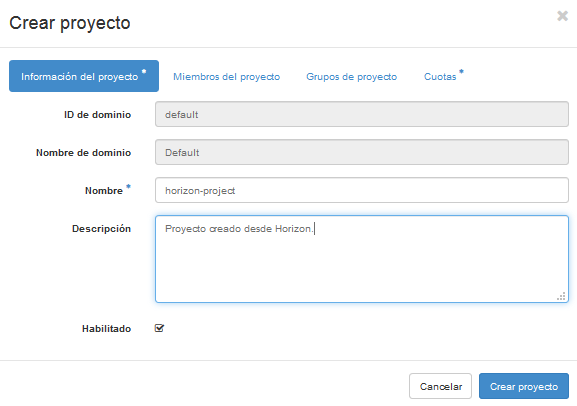
\includegraphics[width=1\textwidth]{imagenes/capitulo6/crear-proyecto-1.PNG}
    \caption{Creación de un proyecto en Horizon.}
	\vspace{0.3cm}
    \label{crear-proyecto-1}
\end{figure}

Vamos a llamarlo “horizon-project”, Fig.\ref{crear-proyecto-1}. La descripción no es necesaria. En las pestañas “Miembros del proyecto” y “Grupos del proyecto” podemos especificar los miembros y grupos del proyecto que deseemos. En este caso dejaremos los que vienen por defecto para después ver como se añaden los que creemos nosotros y no los que se instalaron como demo. Podemos pasar directamente al apartado de “Cuotas”.

La cuota del proyecto es importante ya que se utiliza para determinar que los usuarios de su proyecto no pueden obtener acceso ilimitado a los recursos en la nube. Por lo tanto, podemos limitar la cantidad de instancias, la cantidad de RAM que se puede usar, estableciéndola en 4096 MB por ejemplo, porque tenemos alrededor de 9 GB de RAM solamente tras la instalación de DevStack, la cantidad de direcciones IP flotantes, la cantidad de redes, etc.

Después de imponer las limitaciones que vemos  en la Fig.\ref{crear-proyecto-2}, habremos especificado  las propiedades de cuota del proyecto. Haciendo  clic en “Crear proyecto” crearemos el tenant que se agregará a los que ya existían.

\begin{figure}
    \centering
    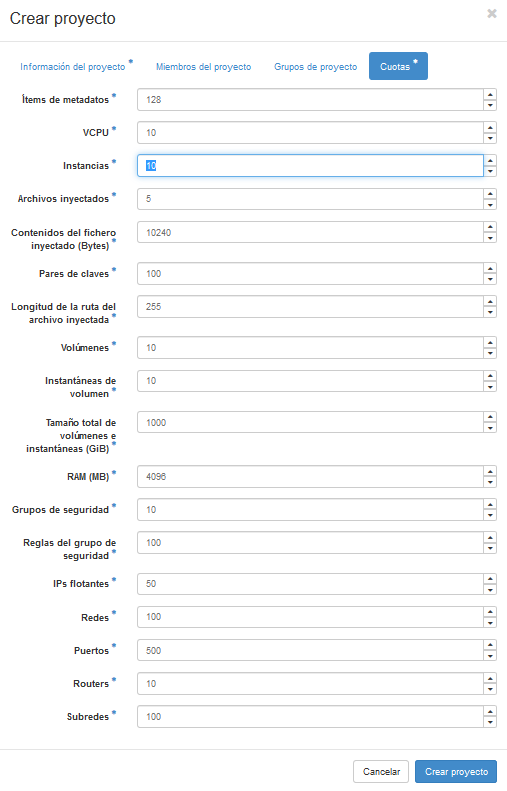
\includegraphics[width=1\textwidth]{imagenes/capitulo6/crear-proyecto-2.PNG}
    \caption{Cuota del proyecto.}
	\vspace{0.3cm}
    \label{crear-proyecto-2}
\end{figure}

\subsection{Creación de usuarios}
El siguiente paso será crear un usuario. Dentro de “Identity” clicamos en “Usuarios” y “Crear usuario”, Fig.\ref{crear-usuario}.

Vamos a darle un nombre, “horizon-user”. No necesitamos una descripción ni un correo electrónico pero sí una contraseña. Los usuarios también deben asignarse a un proyecto, de modo que en la lista “Proyecto principal”, podemos seleccionar el proyecto que acabamos de crear. También podemos definir en el desplegable “Rol”, el tipo de usuario o rol que tendrá. Especificamos que sea \textit{Member}. Un usuario Member puede crear todo lo necesario en el entorno de la nube. Después de especificar las propiedades del usuario, podemos hacer clic en “Crear usuario” y con esto, dicho usuario podrá ya iniciar sesión.

\begin{figure}
    \centering
    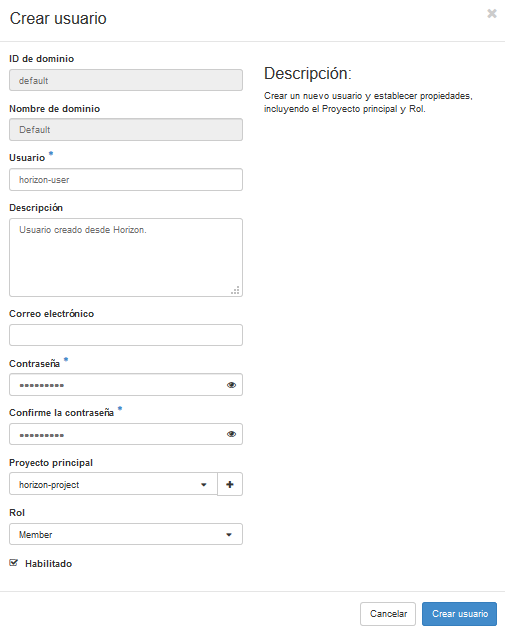
\includegraphics[width=1\textwidth]{imagenes/capitulo6/crear-usuario.PNG}
    \caption{Creación de un usuario.}
	\vspace{0.3cm}
    \label{crear-usuario}
\end{figure}

Las pestañas “Grupos” y “Roles” de “Identity” se usan con menor frecuencia. Sus funciones son las de  agrupar diferentes usuarios y definir nuevos roles respectivamente, pero normalmente para la mayoría de los entornos en la nube, basta con los roles de miembro y administrador.

\jorge{La figura 7.8 se ve muy poco, ponla en apaisado.}

Si cerramos sesión e iniciamos de nuevo pero esta vez con el usuario “horizon-user” creado, entraremos directamente a la vista general del usuario que vemos en la Fig.\ref{acceso-horizon-user}, donde el proyecto se abre de manera predeterminada y en el que podremos ver un reporte del uso y las capacidades de nuestro entorno cloud en cuanto a instancias, RAM y el resto de recursos principales.

\begin{tcolorbox}[colback=red!5!red,colframe=red!75!black]
ESTAS IMÁGENES QUE HAY QUE METER TAN LARGAS, COMO LA DE LOS ENDPOINTS, PROBAR A HACER LA VENTA MAS PEQUEÑA A VER SI ASÍ SALE MEJOR.
\end{tcolorbox}

\begin{figure}
    \centering
    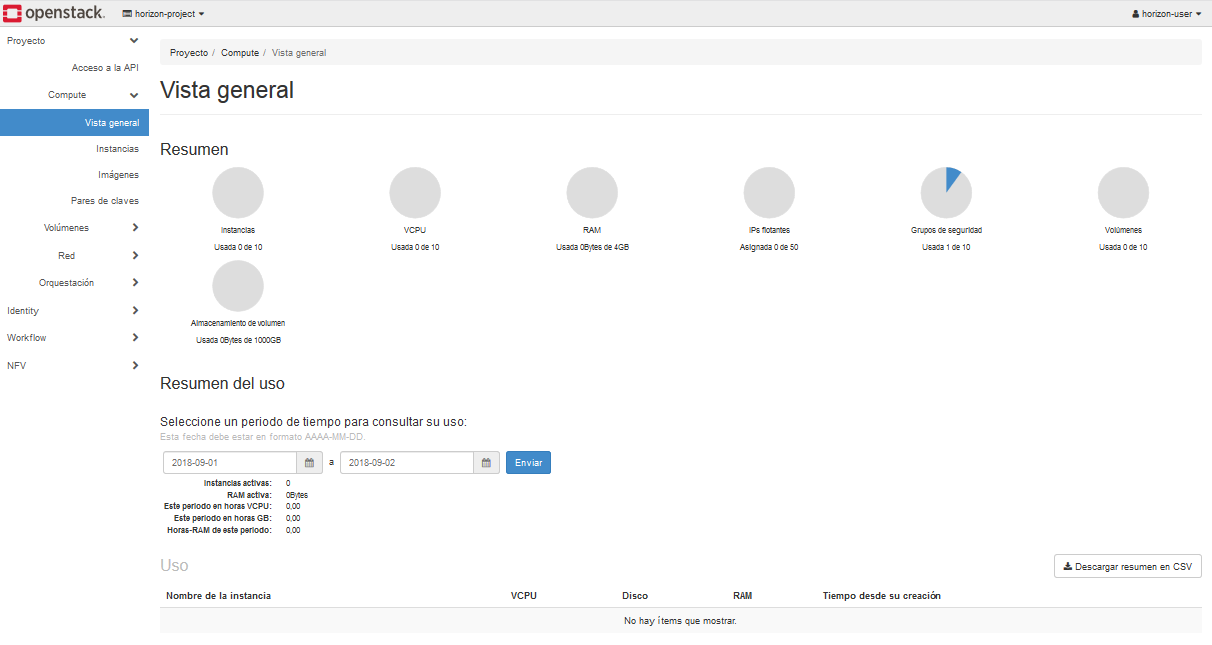
\includegraphics[width=1\textwidth]{imagenes/capitulo6/acceso-horizon-user.PNG}
    \caption{Vista general del proyecto horizon-project.}
	\vspace{0.3cm}
    \label{acceso-horizon-user}
\end{figure}

\subsection{Recursos necesarios para crear una instancia}
En este apartado, vamos a explicar qué se necesita para implementar una instancia en un entorno de nube OpenStack.

Partimos de nuestro \textit{Compute Node}. Dicho nodo ejecuta el hipervisor KVM o cualquier hipervisor que se necesite y se derivará de una instancia, pero las diferentes partes de la instancia provienen de otro lugar. Para ejecutar una instancia se necesitas redes, necesitamos una imagen, ajustes de seguridad y otros. Todos estos requisitos son provistos por diferentes servicios de OpenStack.

La instancia en sí proviene del servicio Nova, que se ocupa de crear las instancias, así como de las capas del hipervisor y de proporcionar seguridad. Luego está la creación de redes. Para encargarnos de las redes, necesitamos configurar Neutron. En Neutron, necesitamos una red privada, que se reservará para un inquilino específico que ejecutará la instancia. Y luego está la imagen, que es proporcionada por el servicio de imágenes Glance.

Y aún hay más. Al proporcionar una instancia, está se ejecuta como una instancia de solo lectura, lo que significa que el almacenamiento será efímero y no se podrá almacenar en ningún lugar, sería similar a arrancar un sistema operativo desde un live CD. Si queremos que una instancia pueda almacenar información en algún lugar, tendremos que gestionar también el almacenamiento de la misma que es proporcionado por el servicio de Cinder.

\begin{figure}
    \centering
    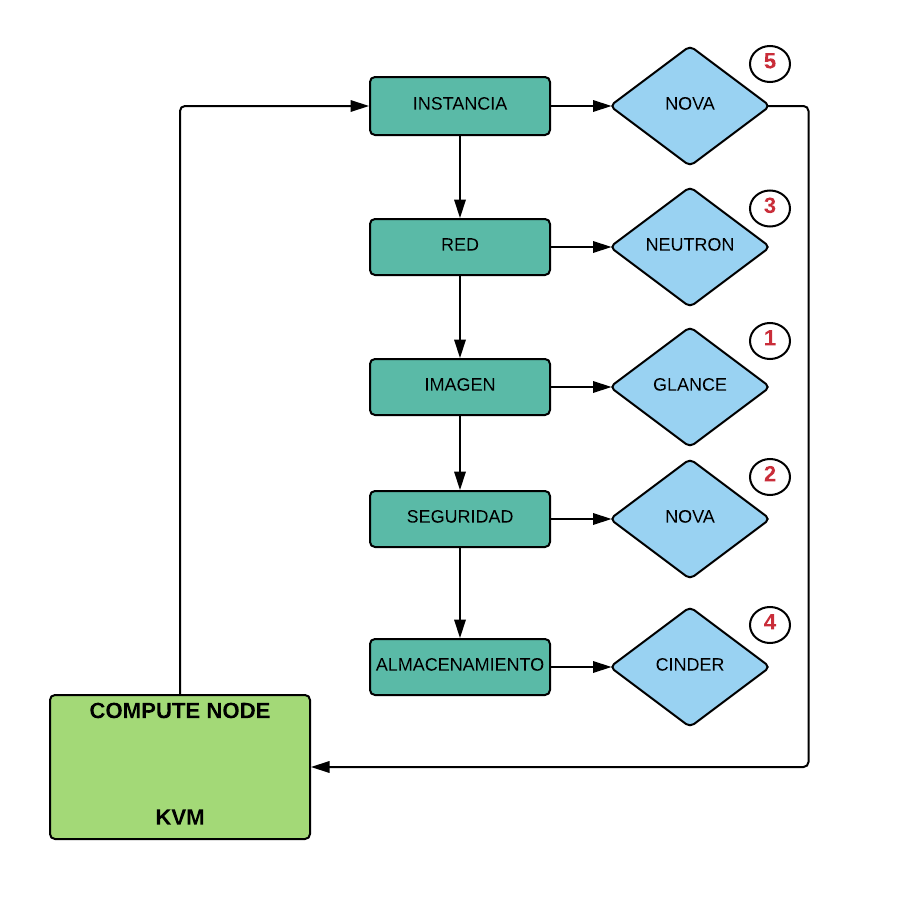
\includegraphics[width=0.7\textwidth]{imagenes/capitulo6/recursosInstancia.png}
    \caption{Recursos necesarios para la creación de una Instancia.}
	\vspace{0.3cm}
    \label{recursosInstancia}
\end{figure}

Así pues si queremos crear una instancia, no es tan simple como arrancarla sin más, necesitamos preparar otras elementos antes. En primer lugar la imagen en Glance que vamos a arrancar, un símil podría ser el ya nombrado de un live CD de Linux. Después, debemos asegurarnos de que en Nova tenemos configurada y activa la seguridad  pues de lo contrario no podremos acceder a la imagen. También tenemos que atender al networking y también al almacenamiento persistente si así lo queremos. Una vez realizadas estas tareas, podremos bootear desde Nova la instancia. Un esquema de los pasos podemos verlo en la Fig.\ref{recursosInstancia}.

De modo que los pasos a seguir son:

\begin{itemize}
\item Configurar la red
\item Asignar direcciones IP flotantes
\item Definir un grupo de seguridad en la nube
\item Crear un par de claves SSH
\item Crear una imagen de Glance
\item Eligir un \textit{flavor}, el cual contendrá las capacidades hardware reservadas para la instancia. 
\item Iniciar la instancia.
\end{itemize}

\subsection{IP flotante} \label{subsec:IP-flotante}
Las redes son una parte muy importante del entorno cloud. Antes incluso de comenzar a crear instancias en nuestra nube, como administradores de un tenant tendremos que crear el entorno de SDN. Esto implica que hemos de asegurarnos de que las instancias se puedan conectar a una red interna privada y también asignar direcciones IP flotantes para que puedan ser alcanzadas externamente.

En primer lugar vamos a definir el concepto de IP flotante en OpenStack. Una dirección IP flotante es un servicio proporcionado por Neutron. No se utiliza para la asignación ningún servicio DHCP ni está configurado de manera estática  dentro de la instancia o la máquina donde se ejecute. De hecho, el sistema operativo anfitrión no tiene idea de que se le asignó una dirección IP flotante. La entrega de paquetes a la interfaz con la dirección flotante asignada es responsabilidad del agente L3 de Neutron. 

A las instancias con una dirección IP flotante asignada se puede acceder desde la red pública mediante la IP flotante.
Una dirección IP flotante y una dirección IP privada se pueden usar al mismo tiempo en una única interfaz de red. Es probable que la dirección IP privada se use para la comunicación o acceso a otras instancias dentro de la red privada mientras que la dirección IP flotante se usará para acceder a la instancia desde redes públicas.

\begin{figure}
    \centering
    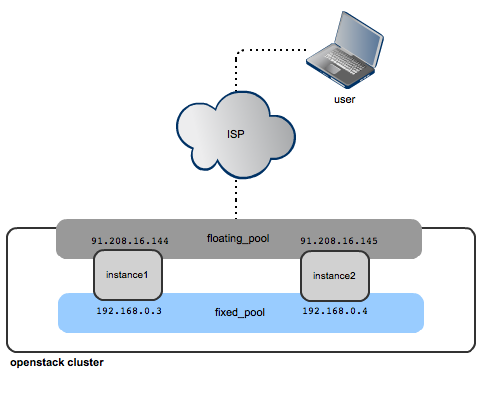
\includegraphics[width=0.7\textwidth]{imagenes/capitulo6/floatingIP.png}
    \caption{Esquema de uso de IPs flotantes.}
	\vspace{0.3cm}
    \footnotesize{Fuente: Mirantis }
    \label{ipsflotantes}
\end{figure}

Para explicar su funcionamiento pondremos un ejemplo de uso. En la Fig.\ref{ipsflotantes} podemos ver un diagrama que esquematiza un posible escenario donde se refleja el tema que estamos tratando. En la parte inferior de esta figura se puede ver que hay dos instancias: instancia 1 e instancia 2, y tienen direcciones IP que provienen de la red privada. La red privada es como una red detrás de un router NAT. Todo lo que está detrás del router NAT no se puede abordar directamente, por lo tanto, no se puede acceder a las direcciones IP 192.168.0.3 y 192.168.0.4 directamente desde Internet. Es por eso que en OpenStack, al crear nuestras SDN para hacer que las instancias sean accesibles, se necesitan direcciones IPs flotantes como se puede ver en la parte superior de la figura.\cite{noauthor_floating_2012}

Por tanto, una dirección IP flotante  es una dirección IP que está reservada para una instancia y está expuesta en el lado externo del router NAT. De este modo, para que el tráfico externo llegue a nuestra instancia creada, el tráfico externo deberá ir directamente a la dirección IP flotante de la instancia y es el router SDN el que se asegura de que todo el tráfico que llega, por ejemplo, a la IP 91.208.16.144, se reenvíe a la 192.168.0.2.

Hay una parte interesante en la configuración de todo esto y es que la dirección IP flotante no es conocida por la instancia como ya hemos comentado, sino que es conocida únicamente por el router SDN que la usa para llegar a la instancia. 

\subsection{Creación de redes}
Ya tenemos configurado un entorno de proyecto con un administrador de proyecto. El siguiente paso es comenzar a trabajar con instancias, Pero antes de que podamos comenzar a trabajar con instancias debemos encargarnos de definir las redes.

Desde dentro de Horizon, en el apartado  “Proyecto-\textgreater Red-\textgreater Redes”, el primer paso será crear una nueva red definida por software. Para hacerlo, hacemos clic en “Crear red” y la le ponemos el nombre “horizon-private-net” %(Fig.\ref{crearRed})
. Esta será nuestra red privada o interna.

\begin{tcolorbox}[colback=green!5!white,colframe=green!75!black]
FALTA FIGURA....................................................

....................................................FALTA FIGURA
\end{tcolorbox}

\begin{comment}
\begin{figure}
    \centering
    \includegraphics[width=0.7\textwidth]{imagenes/capitulo6/crearRed.PNG}
    \caption{Creando una red desde Horizon.}
	\vspace{0.3cm}
    \label{crearRed}
\end{figure}
\end{comment}

Al configurar una SDN, es muy importante hacer una distinción entre la red interna y la red externa. La red interna es a la que se conectarán las máquinas virtuales  que creemos mientras que la red externa es la que nos permitirá conectarnos con nuestra infraestructura de red física.

El siguiente paso es crear una subred desde la pestaña de la misma ventana “Subred”. Vamos a llamarla “horizon-private-subnet”. Esta subred necesita una dirección de red, usaremos 192.170.1.0/24 %como vemos en la Fig.\ref{crearSubRed}. 
Se puede usar cualquier dirección IP que deseemos siempre que sea una dirección IP privada. Esta es la subred que usarán internamente solo las máquinas virtuales y permitirá que las máquinas virtuales en la nube se comuniquen entre sí.

\begin{tcolorbox}[colback=green!5!white,colframe=green!75!black]
FALTA FIGURA....................................................

....................................................FALTA FIGURA
\end{tcolorbox}

\begin{comment}
\begin{figure}
    \centering
    \includegraphics[width=0.7\textwidth]{imagenes/capitulo6/crearSubRed.PNG}
    \caption{Creando una subred desde Horizon.}
	\vspace{0.3cm}
    \label{crearSubRed}
\end{figure}
\end{comment}

En nuestro rango de red IP, es probable que deseemos tener una puerta de enlace o \textit{gateway} también. Podemos especificar la puerta de enlace, pero si no lo hacemos, obtendremos una dirección de puerta de enlace predeterminada, ya que en cualquier red para que las máquinas se comuniquen con el mundo exterior, necesitamos pasarelas en todo momento. En caso de que no queramos una puerta de enlace, podemos hacer clic específicamente en “Deshabilitar puerta de enlace”, pero eso normalmente no es algo que deseemos hacer.

En  la siguiente pestaña tenemos el bloque de  “Detalles de Subred”. En los detalles de la subred podemos especificar el resto de elementos necesarios para especificar nuestra subred. Básicamente esto se reduce a la configuración de DHCP. DHCP se asegurará de que nuestras instancias obtengan una dirección IP por defecto en el rango de subred especificado. En el campo “Pools de asignación”, necesitamos crear una lista de direcciones IP separada por comas con la primera dirección en el grupo de asignación y la última dirección en el grupo de asignación, o una dirección por línea si así lo queremos. En este caso, crearemos un rango de direcciones DHCP válidas dentro de la subred que irá desde la 192.170.1.100 a la 192.170.1.150. %Como evidencia mostramos la Fig.\ref{crearSubRedDetails}.

\begin{tcolorbox}[colback=green!5!white,colframe=green!75!black]
FALTA FIGURA....................................................

....................................................FALTA FIGURA
\end{tcolorbox}

\begin{comment}
\begin{figure}
    \centering
    \includegraphics[width=0.7\textwidth]{imagenes/capitulo6/crearSubRedDetails.PNG}
    \caption{Configuración de DHCP y DNS.}
	\vspace{0.3cm}
    \label{crearSubRedDetails}
\end{figure}
\end{comment}

También podemos especificar el o los servidores DNS en el campo “Servidores DNS”, asignando así un servidor de nombres a las instancias y también podemos crear rutas a host específicos en el campo “Rutas de host”. Normalmente, esto no será necesario ya que la gateway creada por defecto se encargará de ello. Haciendo clic en “Crear” tendremos la red a punto.

En este punto, debemos asegurarnos de que haya también una red pública. La red pública podríamos crearla de forma análoga clicando de nuevo en “Crear red” y habilitándola como red pública después desde el tenant de administrador, pero está red ya se creo en la instalación inicial de manera automática en base a los parámetros de configuración introducidos en el archivo \textit{local.conf} (ver apéndice \ref{chap:manualdeinstalacion}).

Una vez tenemos ambas redes podremos ver que aparecen en nuestro panel.

\begin{tcolorbox}[colback=green!5!white,colframe=green!75!black]
FALTA FIGURA....................................................

....................................................FALTA FIGURA
\end{tcolorbox}

\begin{comment}
\begin{figure}
    \centering
    \includegraphics[width=0.7\textwidth]{imagenes/capitulo6/redesCreadas.PNG}
    \caption{Panel de red.}
	\vspace{0.3cm}
    \label{redesCreadas}
\end{figure}
\end{comment}

\subsection{Creación de routers}
El siguiente paso será establecer una conexión entre la red pública y la red privada para lo cual necesitaremos crear un router. En la pestaña “Proyecto-\textgreater Red-\textgreater Routers” cliclamos en “Crear Router” y nombramos el router a crear como “horizon-router”. 

Además tendremos que seleccionar una red externa que será la red pública creada nombrada como “public”. Haciendo clic en “Crear Router” tendremos el router creado y en la topología de red que vemos en la %Fig.\ref{crearRouter}
aparecerá conectado a la red pública. Si pasamos el cursor sobre el icono “horizon-router”, podemos ver diferentes opciones. De ellas seleccionamos “Añadir interfaz” para agregar una  nueva interfaz que nos permitirá conectar nuestro router también con la red interna “horizon-private-net”, al seleccionarla, automáticamente conecta el router con esa red creando una interfaz que tiene asignada la dirección IP 192.170.1.1, dentro del rango de direcciones de la subred que creamos.

\begin{tcolorbox}[colback=green!5!white,colframe=green!75!black]
FALTA FIGURA....................................................

....................................................FALTA FIGURA
\end{tcolorbox}
\begin{comment}

\begin{figure}
    \centering
    \includegraphics[width=0.7\textwidth]{imagenes/capitulo6/crearRouter.PNG}
    \caption{Creación de un router.}
	\vspace{0.3cm}
    \label{crearRouter}
\end{figure}
\end{comment}


\begin{tcolorbox}[colback=green!5!white,colframe=green!75!black]
FALTA FIGURA....................................................

....................................................FALTA FIGURA
\end{tcolorbox}

\begin{comment}
\begin{figure}
    \centering
    \includegraphics[width=0.7\textwidth]{imagenes/capitulo6/addInterfazRouter.PNG}
    \caption{Añadir interfaz a un router.}
	\vspace{0.3cm}
    \label{addInterfazRouter}
\end{figure}
\end{comment}


\subsection{Implementar una instancia desde Horizon}
Ahora que se ha configurado la red, podemos encargarnos del resto. Para empezar, tendremos que crear un grupo de seguridad o \textit{security group}. El grupo de seguridad es un conjunto de reglas de firewall que se aplicarán desde la nube a una instancia. La idea es que la instancia se genere desde una imagen de Glance. En una imagen de Glance, no se pueden definir las reglas de firewall que deben aplicarse y es por eso que tenemos que definirlas a través de la creación de un grupo de seguridad en la nube.

El siguiente paso por tanto es crear un par de claves SSH (\textit{SSH Key Pair}). SSH key pair consiste en un conjunto de clave pública-privada. La clave privada se mantiene en la estación de trabajo y la clave pública en la instancia, por tanto, el par de claves SSH nos sirve para permitir una conexión segura a la instancia. La otra opción sería acceder a la instancia utilizando contraseñas predeterminadas y nombres de usuario predeterminados lo cual es muy inseguro por lo que utilizando SSH Key Pairs, aumentamos el nivel de seguridad. Estas claves generadas serán las que usemos más tarde para conectarnos a las instancias creadas a través de un terminal.

También necesitamos la imagen de Glance. Una imagen de Glance es como un live CD de Linux. Veremos cómo podemos descargar una imagen usando de Cirros desde la nube.

Por último tenemos el flavor que también tendremos que seleccionar. Un flavor es básicamente el perfil de hardware que elegiremos para nuestra instancia. De este modo, si creamos una instancia de una imagen de Glance, determinaremos cuánta RAM, cuánto espacio en disco, etc., va a usar dicha instancia. Una vez que hayamos seguido este proceso, podremos arrancar la instancia.


En este punto, tenemos una red operativa, lo cual significa que cumplimos con todos los requisitos para implementar instancias desde Horizon. En primer lugar, tendremos que entrar en Horizon como tenant “horizon-user”, un usuario cualquiera, ya que el administrador de la nube no va a derivar instancias para los inquilinos si no que lo harán ellos mismos.

\subsection{Creación de grupos de seguridad}
Lo primero que vamos a crear es un grupo de seguridad. Un grupo de seguridad es un firewall. La razón por la que estamos trabajando con grupos de seguridad en entornos de nube es que, si se derivan las instancias de la nube de forma dinámica, no es posible crear firewalls diferenciados dentro de las instancias de la nube, y es por eso que vamos a definir el firewall desde la nube y asignarlo a las instancias. Para hacerlo, dentro de “Red”, en el apartado de “Grupos de seguridad”. Le daremos el nombre de “horizon-secgroup” tal como vemos en la %Fig.\ref{createSecGroup}

\begin{tcolorbox}[colback=green!5!white,colframe=green!75!black]
FALTA FIGURA....................................................

....................................................FALTA FIGURA
\end{tcolorbox}

\begin{comment}
\begin{figure}
    \centering
    \includegraphics[width=0.7\textwidth]{imagenes/capitulo6/createSecGroup.PNG}
    \caption{Creación de un grupo de seguridad.}
	\vspace{0.3cm}
    \label{createSecGroup}
\end{figure}
\end{comment}

Una vez creado haciendo clic en el “Administar reglas” del campo “Acciones” del grupo de seguridad creado vamos a definir algunas reglas de seguridad. Las reglas de seguridad funcionan de manera similar a como se hacen creando listas de acceso en un router de Cisco por ejemplo. Por defecto, tal como aparece en la %Fig.\ref{crearReglas}
, tenemos permitido tráfico saliente permitido en IPv4 a cualquier parte, y tenemos tráfico saliente permitido en IPv6 en cualquier lugar, además, de manera predeterminada el tráfico entrante no está permitido.

\begin{tcolorbox}[colback=green!5!white,colframe=green!75!black]
FALTA FIGURA....................................................

....................................................FALTA FIGURA
\end{tcolorbox}

\begin{comment}
\begin{figure}
    \centering
    \includegraphics[width=0.7\textwidth]{imagenes/capitulo6/crearReglas.PNG}
    \caption{Reglas por defecto y creación de nuevas reglas.}
	\vspace{0.3cm}
    \label{crearReglas}
\end{figure}
\end{comment}


Podemos crear reglas nuevas pulsando en “Agregar regla”. En primer lugar agregaremos una regla del tipo “Todos los ICMP” cuyos parámetros vemos en la %Fig.\ref{reglaICMP}
. Esta regla especificamos en el campo “Dirección”, “Entrante”, para indicar que se trata de una regla acerca del tráfico ICMP de entrada, en el campo “Remoto” seleccionamos “CIDR” y como CIDR (\textit{Classless Inter-Domain Routing}) 0.0.0.0/0, indicando así que permitimos cualquier dirección IP, permitiendo de este modo que las instancias creadas puedan ser alcanzadas por cualquiera.

\begin{tcolorbox}[colback=green!5!white,colframe=green!75!black]
FALTA FIGURA....................................................

....................................................FALTA FIGURA
\end{tcolorbox}

\begin{comment}
\begin{figure}
    \centering
    \includegraphics[width=0.7\textwidth]{imagenes/capitulo6/reglaICMP.PNG}
    \caption{Creación de una regla para el tráfico ICMP.}
	\vspace{0.3cm}
    \label{reglaICMP}
\end{figure}
\end{comment}

Creamos una regla más del mismo modo. Esta vez vamos a permitir el tráfico HTTP para lo que en “Regla” marcamos “HTTP” con “CIDR”, 0.0.0.0/0, y una última, sobre el tráfico SSH con los mismos parámetros, la cual es de vital importancia ya que a las instancias, de manera predeterminada, accederemos como usuarios vía SSH y tenemos que permitirlo en el firewall. Una creadas todas se mostrarán en el panel como se aprecia en la %Fig.\ref{reglasCreadas}.

\begin{comment}
\begin{figure}
    \centering
    \includegraphics[width=0.7\textwidth]{imagenes/capitulo6/reglasCreadas.PNG}
    \caption{Panel de grupos de seguridad con las reglas creadas.}
	\vspace{0.3cm}
    \label{reglasCreadas}
\end{figure}
\end{comment}

\subsection{Creación de IPs flotantes}
En el siguiente paso trabajaremos con direcciones IP flotantes. Una dirección IP flotante es una dirección IP que se utilizará para hacer que la instancia sea accesible desde el exterior. La razón por la que las necesitamos es que por defecto, las instancias son visibles sólo en la red privada. Si solo están en la red privada, nadie externo podrá acceder a ellas, y es por eso que debemos usar direcciones IP flotantes.

Por tanto, una dirección IP flotante es una dirección IP en la nube, y todo lo que entra en la dirección IP flotante se reenviará a la dirección IP de la instancia. Esto significa que la dirección IP flotante debe estar disponible en la red externa, que es la red pública que creamos como “public”, lo que implica que debemos asegurarnos de que cuando se está construyendo la nube, la red pública tenga una cantidad significativa de direcciones IP disponibles. Por esto motivo, en la preparación de los servidores creamos una interfaz virtual de la tarjeta de red disponible, ya que al sólo tener una, sólo podíamos disponer de una dirección IP flotante. De este modo conseguimos tener un pool de direcciones IPs flotantes disponibles para asignar a las instancias.

Comenzamos moviéndonos al apartado “Proyecto-\textgreater Red-\textgreater IPs flotantes” y clicamos en “Asignar IP al proyecto” para asignar una IP flotante al proyecto, que se creará automáticamente del pool que habíamos creado como vemos en la %Fig\ref{crearIPflotante}
. Necesitaremos una IP flotante por cada instancia que creemos, luego siguiendo el mismo proceso podemos crear tantas como nuestra quota nos permita. 

\begin{tcolorbox}[colback=green!5!white,colframe=green!75!black]
FALTA FIGURA....................................................

....................................................FALTA FIGURA
\end{tcolorbox}

\begin{comment}
\begin{figure}
    \centering
    \includegraphics[width=0.7\textwidth]{imagenes/capitulo6/crearIPflotante.PNG}
    \caption{Creación de una IP flotante.}
	\vspace{0.3cm}
    \label{crearIPflotante}
\end{figure}
\end{comment}

\subsection{Creación de pares de claves público-privada}
Para llegar al paso de la %Fig.\ref{horizon-keypair} 
iremos ahora al apartado  “Proyecto-\textgreater Compute”, donde vamos a encargarnos  de las instancias. Antes de que podamos derivar una instancia, necesitamos un par de claves SSH, por tanto en primer lugar clicamos en “Pares de claves” y dentro del apartado “Crear Par de de Claves”. Tenemos que darle un nombre que será “horizon-keypair” y pulsar en “Crear Par de Claves” para que se genere

\begin{tcolorbox}[colback=green!5!white,colframe=green!75!black]
FALTA FIGURA....................................................

....................................................FALTA FIGURA
\end{tcolorbox}


\begin{comment}
\begin{figure}
    \centering
    \includegraphics[width=0.7\textwidth]{imagenes/capitulo6/horizon-keypair.PNG}
    \caption{Creación de un par de claves.}
	\vspace{0.3cm}
    \label{horizon-keypair}
\end{figure}
\end{comment}

Una vez creada podremos descargarla para usarla después. Esta clave privada es una clave que debe estar disponible y por tanto almacenada en la estación de trabajo del usuario final.

Si nos encontramos en el PC que vaya a hacer de estación de trabajo, en mi caso mi ordenador personal, vamos al directorio “.ssh” y copiaremos la clave privada generada para alojarla en la estación de trabajo:

\begin{lstlisting}[style=Consola]
atj@wimunet4:~/devstack$$ ls -l | grep key
-rw-rw-r-- 1 atj atj 1679 sep  6 10:52 horizon-keypair
atj@wimunet4:~/devstack$ chmod 400 horizon-keypair
atj@wimunet4:~/devstack$ ls -l | grep MyKeyP
-r-------- 1 atj atj 1679 sep  6 10:52 horizon-keypair
atj@wimunet4:~/devstack$ cp horizon-keypair /home/atj/.ssh
\end{lstlisting}

“ls -l” muestra los permisos que necesitamos. Esta clave privada será utilizada por el usuario final para conectar a los servidores que tienen una copia de la clave pública disponible, necesario para entrar a las instancias que se implementarán en OpenStack. También hemos cambiado el tipo de permisos ya que inicialmente no era el correcto. La clave privada debe ser altamente segura, por lo que es aconsejable cambiarle los permisos.

\subsection{Creación de imágenes}
El siguiente paso está encaminado a la creación de imágenes. Necesitamos las imágenes porque las instancias de la nube de OpenStack no están instaladas, sino que se implementan. La instalación funciona para un centro de datos tradicional, donde un administrador pasa por todas las diferentes opciones para instalar una máquina virtual. Eso no es lo que se hace en OpenStack. En OpenStack, la implementamos utilizando una imagen lista para ser usada.

En nuestro caso vamos a usar la imagen de Cirros, que es más ligera y por motivos de capacidad la más aconsejable. Antes de poder usarla necesitamos realizar la descarga de la imagen desde la máquina en la que se esté ejecutando Horizon, en nuestro caso nuestro servidor. Para iniciar la descarga en caso de que no hubiesemos incorporado la misma en el script de configuración incial o quisieramos otra podemos escribir desde una consola dentro de la máquina que aloja OpenStack:
% o ponerla en el script de configuración

\begin{lstlisting}[style=Consola]
stack@wimunet4:~/devstack$ wget http://download.cirros-cloud.net/0.4.0/cirros-0.4.0-x86_64-disk.img
\end{lstlisting}

Cirros es una imagen de nube que nos permitirá probar la implementación de instancias en una nube de OpenStack o en cualquier otra nube. Esta imagen no sería la que usaríamos en un entorno cloud de producción, pero es altamente aconsejable para nuestro propósito debido a que las imágenes de cirros son realmente pequeñas, por lo que no supondrá una gran capacidad de los recursos que tenemos disponibles en nuestra máquina. Por supuesto, existen también otras imágenes en la nube disponibles \cite{noauthor_openstack_nodate-7}, pero estas requieren más requisitos hardware y suelen modificarse para usarse en entornos de producción.

Una vez que tenemos la imagen en la nube disponible, podemos volver a Horizon para crear nuestra imagen con los parámetros de la %Fig.\ref{crearImagenHorizon}
, y dentro de  “Proyecto-\textgreater Compute-\textgreater Imágenes” hacer clic en “Crear imagen”. Vamos a llamar “horizon-cirros” y especificamos el tipo de formato, que será QCOW2. QCOW2 es un formato de imagen de nube común, tenemos otros formatos disponibles, también, pero de nuevo no es recomendable usar ninguno de ellos ya que son para entornos específicos que no deseamos usar por el momento. Tenemos una opción en el campo “Compartir imagen” interesante, ya que permite establecer una imagen como protegida o no. Puesto que es una imagen que como usuario tenant, queremos que esté disponible para todos los demás, marcaremos la opción “No”. Después de hacerlo, haciendo clic en “Create Image” importaremos la imagen a nuestro entorno de nube OpenStack. 

\begin{tcolorbox}[colback=green!5!white,colframe=green!75!black]
FALTA FIGURA....................................................

....................................................FALTA FIGURA
\end{tcolorbox}


\begin{comment}
\begin{figure}
    \centering
    \includegraphics[width=0.7\textwidth]{imagenes/capitulo6/crearImagenHorizon.PNG}
    \caption{Creación de una imagen: Detalles.}
	\vspace{0.3cm}
    \label{crearImagenHorizon}
\end{figure}
\end{comment}

\subsection{Creación de instancias}
Una vez que la imagen se ha importado con éxito, vamos a “Proyecto-\textgreater Compute-\textgreater Instancias” y seleccionamos “Lanzar instancia”. Esto nos lleva a una lista de diferentes items que podemos configurar al iniciar una instancia. Todo lo que está marcado con un asterisco es obligatorio y el resto opcional como podemos ver en la %Fig.\ref{creandoInstancia}
, donde en primer lugar le damos un nombre a la instancia, “horizon-instance-1”. La opción “Count” permite lanzar más instancias al mismo tiempo. Haciendo clic en “Siguiente” pasaremos a especificar el origen de arranque, que será nuestra imagen importada, además podemos decidir si crear un volumén que se asiganará a esa instancia y si tras eliminar la misma mantendremos el volumen o no quedando así la configuración de la %Fig.\ref{origenInstancia}
.

\begin{tcolorbox}[colback=green!5!white,colframe=green!75!black]
FALTA FIGURA....................................................

....................................................FALTA FIGURA
\end{tcolorbox}


\begin{comment}
\begin{figure}
    \centering
    \includegraphics[width=0.7\textwidth]{imagenes/capitulo6/origenInstancia.PNG}
    \caption{Creación de una imagen: Origen.}
	\vspace{0.3cm}
    \label{origenInstancia}
\end{figure}
\end{comment}


Pulsamos “Siguiente” y seleccionamos el “Sabor” (del ingés \textit{flavor}) para especificar el perfil de hardware que va a utilizar nuestra instancia. Podríamos crear nuestros propios flavors si así lo queremos, de hecho, para tener un flavor que se ajuste más a los requisitos que necesite nuestra máquina vamos a crear el que usaremos a continuación del siguiente modo:

\begin{lstlisting}[style=Consola]
stack@wimunet4:~/devstack$ source openrc admin admin
stack@wimunet4:~/devstack$ openstack flavor create --ram 512 --disk 4 --vcpus 1 m1.little
\end{lstlisting}

El motivo de autenticarnos antes como usuario administrador del entorno, es que este flavor pueda estar disponible para cualquier usuario ya que si lo hacemos desde un tenant específico, como por ejemplo el que estamos usando, horizon-user, sólo estaría disponible para el projecto horizon-project. De acuerdo a la configuración introducida, la imagen que asociemos a este flavor de acuerdo al orden de parámetros introducido tendrá una RAM de 512 MB, 4 GB de disco reservada para la partición /root, una única CPU virtual y como nombre \textit{m1.little}. De igual modo podríamos haberlo hecho desde horizon autenticándonos como admin dentro del apartado “Proyecto-\textgreater Compute-\textgreater Instancias-\textgreater Crear Sabor”. 

Una vez creado, podemos continuar con la creación de la instancia y seleccionarlo dentro de las opciones disponibles en el apartado flavor %(Fig.\ref{flavorInstance})
.

\begin{tcolorbox}[colback=green!5!white,colframe=green!75!black]
FALTA FIGURA....................................................

....................................................FALTA FIGURA
\end{tcolorbox}


\begin{comment}
\begin{figure}
    \centering
    \includegraphics[width=0.7\textwidth]{imagenes/capitulo6/flavorInstance.PNG}
    \caption{Creación de una imagen: Sabor.}
	\vspace{0.3cm}
    \label{flavorInstance}
\end{figure}
\end{comment}

Con esta configuración ya podríamos crear la instancia pero vamos a especificar algunos parámetros de configuración más. Ahora, como vemos en la %Fig.\ref{redesInstancia}
iremos al apartado “Redes” dentro de las opciones de creación de la instancia veremos las redes que se han creado. Necesitamos que esté disponible en “horizon-private-net” para asignar las instancias que creamos a la red interna y luego hacerlas accesibles a través de una dirección IP flotante. 

\begin{tcolorbox}[colback=green!5!white,colframe=green!75!black]
FALTA FIGURA....................................................

....................................................FALTA FIGURA
\end{tcolorbox}


\begin{comment}
\begin{figure}
    \centering
    \includegraphics[width=0.7\textwidth]{imagenes/capitulo6/redesInstancia.PNG}
    \caption{Creación de una imagen: Redes.}
	\vspace{0.3cm}
    \label{redesInstancia}
\end{figure}
\end{comment}


No necesitamos asignar puertos por lo que pasamos a “Grupos de Seguridad”. Es imporante asignarle el grupo creado, pues de lo contrario tendremos una instancia que no será accesible en absoluto. Hacemos clic en la flecha hacia arriba para asignar el grupo “horizon-secgroup” que aparece en la %Fig\ref{secgroupInstancia}
como grupo de seguridad a la instancia. 

\begin{tcolorbox}[colback=green!5!white,colframe=green!75!black]
FALTA FIGURA....................................................

....................................................FALTA FIGURA
\end{tcolorbox}


\begin{comment}
\begin{figure}
    \centering
    \includegraphics[width=0.7\textwidth]{imagenes/capitulo6/secgroupInstancia.PNG}
    \caption{Creación de una imagen: Grupos de Seguridad.}
	\vspace{0.3cm}
    \label{secgroupInstancia}
\end{figure}
\end{comment}


Finalmente en el apartado “Pares de Claves” elegimos “horizon-keypair” y ya podremos cargar la instancia pulsando en el botón “Ejecutar Instancia” de la %Fig.\ref{keyInstancia}
.


\begin{tcolorbox}[colback=green!5!white,colframe=green!75!black]
FALTA FIGURA....................................................

....................................................FALTA FIGURA
\end{tcolorbox}


\begin{comment}
\begin{figure}
    \centering
    \includegraphics[width=0.7\textwidth]{imagenes/capitulo6/keyInstancia.PNG}
    \caption{Creación de una imagen: Par de Claves.}
	\vspace{0.3cm}
    \label{keyInstancia}
\end{figure}
\end{comment}


\subsection{Creación de volúmenes de almacenamiento para las instancias}
\begin{tcolorbox}[colback=red!5!red,colframe=red!75!black]
Quitar la parte de creación de un volumen anterior y meterla aquí.
\end{tcolorbox}



%“”
%“”
%“”
%“”
\section{Configuración de un escenario mediante la CLI}
En este apartado vamos a ver como se puede crear también un escenario como en el caso anterior, pero esta vez desde línea de comandos. Puesto que hemos ido explicando y motivando cada paso en el apartado anterior, vamos a ir directos aquí a las pasos a seguir para alcanzar nuestro objetivo, listando los comandos necesarios para la consecución del acceso a las instancias.

La lista de comandos de OpenStack para administrar la CLI se puede consultar en la documentación pertinente.\cite{noauthor_command_nodate}

Para automatizar el proceso que aquí veremos y ver así la evolución en la administración de OpenStack de la que hablábamos en la sección \ref{subchap:heat} hemos creado un script en bash con el nombre \textit{cli\_creacion\_escenario.sh}. Este script podremos verlo en el apéndice \ref{chap:creacionescenariobash}.

\subsection{Credenciales}
Lo primero que debemos hacer al acceder a la CLI, es autenticarnos con las credenciales de OpenStack de aquel usuario con el que queramos acceder a nuestro entorno. Cuando creamos un usuario, Keystone almacena en su base de datos las credenciales del mismo. Para acceder a ellas y autenticarnos, en este caso como usuario administrados, se indica el nombre del proyecto y el usuario que tenemos:

\begin{lstlisting}[style=Consola]
stack@wimunet4:~/devstack$ source openrc admin admin
\end{lstlisting}

Para establecer las variables de entorno requeridas para los clientes desde la CLI de OpenStack, se debe crear un archivo de entorno llamado archivo \textit{openrc.sh} que en nuestro caso se proporciona al instalar DevStack. Este archivo de entorno específico del proyecto contiene las credenciales que utilizan todos los servicios de OpenStack. De este modo, las variables de entorno se establecen para nuestro \textit{shell} actual. Las variables permiten que los comandos del cliente OpenStack se comuniquen con los servicios OpenStack que se ejecutan en la nube.\cite{noauthor_openrc_nodate}

\subsection{Creación de proyectos o tenants}
\begin{lstlisting}[style=Consola]
stack@wimunet4:~/devstack$ openstack project create --description 'Escenario creado con cli' cli-project --domain default
\end{lstlisting}

\begin{lstlisting}[style=Consola]
stack@wimunet4:~/devstack$ openstack quota set cli-project --instances 10
stack@wimunet4:~/devstack$ openstack quota set cli-project --ram 4096 
\end{lstlisting}

\subsection{Creación de usuarios}
\begin{lstlisting}[style=Consola]
stack@wimunet4:~/devstack$ openstack user create --project cli-project --password temporary cli-user
\end{lstlisting}

\begin{lstlisting}[style=Consola]
stack@wimunet4:~/devstack$ openstack role add --user cli-user --project cli-project Member
\end{lstlisting}

\subsection{Creación de redes}
Vamos a ver en este apartado como crear elementos de conectividad de red, en concreto redes y subredes desde la CLI.

Para crear una red escribimos el siguiente comando:

\begin{lstlisting}[style=Consola]
stack@wimunet4:~/devstack$ openstack network create cli-private-net 
\end{lstlisting}

Se nos devolverá:

\begin{tcolorbox}[colback=green!5!white,colframe=green!75!black]
FALTA FIGURA....................................................

....................................................FALTA FIGURA
\end{tcolorbox}

De este modo crearemos una red llamada \textit{cli-private-net}. No necesitamos propiedades adicionales puesto que estas se declaran en la subred. Así pues este será el siguiente paso:

\begin{lstlisting}[style=Consola]
stack@wimunet4:~/devstack$ openstack subnet create --network cli-private-net --subnet-range 192.168.20.0/24 cli-private-subnet
\end{lstlisting}

Donde los parámetros que aparecen indican:
\begin{itemize}
\item --network cli-private-net. La red a la que queremos asociar la subred.
\item --subnet-range 192.168.20.0/24. El rango de la subred.
\item cli-private-subnet. Nombre que le hemos dado a la subred.
\end{itemize}

Con esto se nos devolverán los parámetros para la subred creada:

\begin{tcolorbox}[colback=green!5!white,colframe=green!75!black]
FALTA FIGURA....................................................

....................................................FALTA FIGURA
\end{tcolorbox}

\subsection{Creación de routers}
Para hacer las redes creadas accesibles necesitamos crear un router.

\begin{lstlisting}[style=Consola]
stack@wimunet4:~/devstack$ openstack router create cli-router
\end{lstlisting}

Para tener acceso a la subred \textit{cli-private-subnet} necesitamos conectar el router creado a esta subred.

\begin{lstlisting}[style=Consola]
stack@wimunet4:~/devstack$ openstack router add subnet cli-router cli-private-subnet
\end{lstlisting}

Y también a la red pública que ya teníamos creada cuyo nombre es \textit{public} con el siguiente comando y el parámetro --external-gateway para indicar que se trata de la puerta de enlace a la red externa.

\begin{lstlisting}[style=Consola]
stack@wimunet4:~/devstack$ openstack router set cli-router --external-gateway public
\end{lstlisting}

Podemos una vez realizada la configuración de los parámetros de red ver como queda la configuración del router como se ve en la Fig. mediante el siguiente comando:

\begin{lstlisting}[style=Consola]
stack@wimunet4:~/devstack$ openstack show cli-router
\end{lstlisting}

\begin{tcolorbox}[colback=green!5!white,colframe=green!75!black]
FALTA FIGURA....................................................

....................................................FALTA FIGURA
\end{tcolorbox}

\subsection{Creación de grupos de seguridad}
Ahora vamos a ver como crear un grupo de seguridad que como sabemos hará las veces de firewall para las instancias:

\begin{lstlisting}[style=Consola]
stack@wimunet4:~/devstack$ openstack security group create cli-secgroup
\end{lstlisting}

Con esto habremos creado un grupo de seguridad llamado \textit{cli-secgroup}. Para que actúe como nosotros queremos, crearemos una serie de reglas que permitan el tráfico que deseamos y el resto no. Por defecto, todo el tráfico saliente esta permitido. Para el entrante:

\begin{lstlisting}[style=Consola]
stack@wimunet4:~/devstack$ openstack  security group rule create --remote-ip 0.0.0.0/0 --protocol tcp --dst-port 22  --ingress cli-secgroup
stack@wimunet4:~/devstack$ openstack  security group rule create --remote-ip 0.0.0.0/0 --protocol icmp --ingress cli-secgroup
stack@wimunet4:~/devstack$ openstack  security group rule create --remote-ip 0.0.0.0/0 --protocol tcp --dst-port 80:80  --ingress cli-secgroup
\end{lstlisting}

Donde hemos creado tres reglas de seguridad asignadas al grupo de seguridad \textit{cli-group} que permiten en tráfico ICMP, SSH y HTTP desde cualquier dirección.

Podemos consultar si las reglas del grupo se han creado con éxito escribiendo:

\begin{lstlisting}[style=Consola]
stack@wimunet4:~/devstack$ openstack security group show cli-secgroup
\end{lstlisting}

Que nos devolverá:

\begin{tcolorbox}[colback=green!5!white,colframe=green!75!black]
FALTA FIGURA....................................................

....................................................FALTA FIGURA
\end{tcolorbox}




\subsection{Creación de IPs flotantes}
Necesitamos también crear IPs flotantes para poder acceder remotamente a las instancias.

\begin{lstlisting}[style=Consola]
stack@wimunet4:~/devstack$ openstack floating ip create public
\end{lstlisting}

Y nos devolverá la IP flotante creada.

\begin{tcolorbox}[colback=green!5!white,colframe=green!75!black]
FALTA FIGURA....................................................

....................................................FALTA FIGURA
\end{tcolorbox}

Este paso lo repetiremos las veces que sea necesaria, tantas como IPs flotantes necesitemos. Un listado de todas las IPs flotantes que tenemos podemos obtenerlo escribiendo en la CLI:

\begin{lstlisting}[style=Consola]
stack@wimunet4:~/devstack$ openstack floating ip list
\end{lstlisting}

Que nos devolverá la lista de IPs flotantes disponibles.

\begin{tcolorbox}[colback=green!5!white,colframe=green!75!black]
FALTA FIGURA....................................................

....................................................FALTA FIGURA
\end{tcolorbox}

\subsection{Creación de pares de claves público-privada}
Vamos a crear ahora una clave para el acceso a las instancias vía SSH que llamaremos \textit{cli-keypair} y guardaremos como \textit{cli-keypair.pem} para su posterior uso cuando queramos acceder a las instancias a las que se les haya asignado esa clave:

\begin{lstlisting}[style=Consola]
stack@wimunet4:~/devstack$ openstack keypair create cli-keypair > cli-keypair.pem
stack@wimunet4:~/devstack$ chmod 0600 cli-keypair.pem
stack@wimunet4:~/devstack$ ssh-add cli-keypair.pem
\end{lstlisting}

Además como vemos hemos modificado los permisos de la clave creada para que sea más segura, pues no es algo a lo que queramos que todos los usuarios tengan acceso, y la hemos añadido a la lista de claves ssh.

Para comprobar que se ha creado correctamente podemos escribir:
\begin{lstlisting}[style=Consola]
stack@wimunet4:~/devstack$ openstack keypair list
\end{lstlisting}

Y veremos (Fig.) como aparece disponible con su correspondiente huella digital o \textit{fingerprint}.


\subsection{Creación de imágenes}
% como user
Almacenaremos todas la imágenes que queramos descargar en la carpeta \textit{images} creada para tal fin:

\begin{lstlisting}[style=Consola]
stack@wimunet4:~/devstack$ mkdir image
\end{lstlisting}

Para preparar la imagen de Cirros la descargamos del repositorio de imágenes de OpenStack:

\begin{lstlisting}[style=Consola]
stack@wimunet4:~/devstack$ wget https://download.cirros-cloud.net/0.4.0/cirros-0.4.0-x86_64-disk.img
\end{lstlisting}

Aunque no es estrictamente necesario al no ser que obtenemos por la descarga de otra imagen puesto que en el archivo de configuración \textit{local.conf} que recordemos podemos ver en el apéndice \ref{chap:manualdeinstalacion} ya impusimos la descarga automática de la misma.

Para crear la imagen escribimos:

\begin{lstlisting}[style=Consola]
stack@wimunet4:~/devstack$ openstack image create --disk-format qcow2 --min-disk 2 --file /opt/stack/devstack/images/cirros-0.4.0-x86_64-disk.img  --private cli-cirros
\end{lstlisting}

Con estemos comando estamos indicando que queremos crear una imagen de las siguientes características:
\begin{itemize}
\item --disk-format. Formato \textit{qcow2} que es el predeterminado para los entornos cloud.
\item --min-disk 2. Creando así un disco de al menos 2 GB.
\item --file /opt/stack/devstack/images/cirros-0.4.0-x86\_64-disk.img. Para indicar la ruta en la que se encuentra la imagen de cirros.
\item --private. Indicamos que la imagen sea privada y por tanto sólo disponible para este proyecto.
\item cli-cirros. Nombre que damos a la imagen creada.
\end{itemize}

Después de introducir el comando podremos ver que OpenStack a creado nuestra imagen donde vemos las propiedades de la misma.
\begin{tcolorbox}[colback=green!5!white,colframe=green!75!black]
FALTA FIGURA....................................................

....................................................FALTA FIGURA
\end{tcolorbox}

Podemos comprobar que efectivamente se ha creado listando las imágenes de las que disponemos:

\begin{lstlisting}[style=Consola]
stack@wimunet4:~/devstack$ openstack image list
\end{lstlisting}

Entre las que podemos ver la que acabamos de crear entre otras.

\begin{tcolorbox}[colback=green!5!white,colframe=green!75!black]
FALTA FIGURA....................................................

....................................................FALTA FIGURA
\end{tcolorbox}



\subsection{Creación de instancias}
\begin{lstlisting}[style=Consola]
stack@wimunet4:~/devstack$ nova boot --flavor m1.little --image cli-cirros --key-name cli-keypair --security-groups cli-secgroup --nic net-name=cli-private-subnet cli-instance-1
\end{lstlisting}

Parámetros:
\begin{itemize}
\item --flavor
\item --image
\item --key-name
\item --security-groups
\item -nic
\item cli-instance-1
\end{itemize}





\subsection{Creación de volúmenes de almacenamiento para las instancias}
\begin{lstlisting}[style=Consola]
stack@wimunet4:~/devstack$ openstack volume create --image cli-cirros \
  --size 8 --availability-zone nova cli-cirros-volume
\end{lstlisting}

\begin{lstlisting}[style=Consola]
stack@wimunet4:~/devstack$ 
openstack server add volume cli-instance-1 \
  cli-cirros-colume --device /dev/vdb
\end{lstlisting}





\section{Orquestación de NFV con Heat}
\subsection{Configuración de un escenario con Heat}
\subsection{Orquestación de instancias con Heat}
\begin{lstlisting}[style=Consola]
heat_template_version: 2013-05-23

description: >
   HOT (Heat Orchestration Template)

parameters:
  key_name:
    type: string
    description: Nombre de una keypair existente para ser usada por las instancias.
    default: cli-keypair
    constraints:
      - custom_constraint: nova.keypair
        description: Debe ser una key-pair conocida por Nova.
  flavor:
    type: string
    description: Flavor para las intancias creadas.
    default: m1.little # 1 vCPU - 512 MB RAM - 4 GB Disk
    constraints:
      - custom_constraint: nova.flavor
        description: Debe ser un flavor conocido por Nova.
  image:
    type: string
    description: Nombre de la imagen usda para crear la instancia.
    default: cli-cirros
    constraints:
      - custom_constraint: glance.image
        description: Debe ser una imagen conocida por Glance.
  netID:
    type: string
    description: El ID de la red a la que se conecte.
    default: e0f00c21-1ac0-49ae-a4cc-e37aa998fd44
    
resources:
  asg:
    type: OS::Heat::AutoScalingGroup
    properties:
      resource:
        type: OS::Nova::Server
        properties:
          key_name: { get_param: key_name }
          image: { get_param: image }
          flavor: { get_param: flavor }
          networks: [{network: {get_param: netID} }]
          metadata: {"metering.stack": {get_param: "OS::stack_id"}}
      min_size: 1
      desired_capacity: 1
      max_size: 3

  scale_up_policy:
    type: OS::Heat::ScalingPolicy
    properties:
      adjustment_type: change_in_capacity
      auto_scaling_group_id: {get_resource: asg}
      cooldown: 60
      scaling_adjustment: 1
      
  scale_down_policy:
    type: OS::Heat::ScalingPolicy
    properties:
      adjustment_type: change_in_capacity
      auto_scaling_group_id: {get_resource: asg}
      cooldown: 60
      scaling_adjustment: '-1'
      
  cpu_alarm_high:
    type: OS::Ceilometer::Alarm
    properties:
      description: Levantar instancia si el uso de la CPU es mayor del 50% durante un minuto.
      meter_name: cpu_util
      statistic: avg
      period: 60
      evaluation_periods: 1
      threshold: 50
      alarm_actions:
        - {get_attr: [scale_up_policy, alarm_url]}
      matching_metadata: {'metadata.user_metadata.stack': {get_param: "OS::stack_id"}}
      comparison_operator: gt

  cpu_alarm_low:
    type: OS::Ceilometer::Alarm
    properties:
      description: Apagar instancia si el uso de la CPU es menor del 15% durante diez minutos.
      meter_name: cpu_util
      statistic: avg
      period: 600
      evaluation_periods: 1
      threshold: 15
      alarm_actions:
        - {get_attr: [scale_down_policy, alarm_url]}
      matching_metadata: {'metadata.user_metadata.stack': {get_param: "OS::stack_id"}}
      comparison_operator: lt
  ceilometer_query:
    value:
      str_replace:
        template: >
          ceilometer statistics -m cpu_util
          -q metadata.user_metadata.stack=stackval -p 600 -a avg
        params:
          stackval: { get_param: "OS::stack_id" }
description: >
      Esto es una query para query de Ceilometer para las estadisticas
      de metricas sobre el util de la cpu.
      Muestras sobre las instancias de OS::Nova::Server estan en este stack.
      El parametro -q selecciona las muestras de acuerdo a los metadatos
      objetivo.
      Cuando los metadatos de una VM incluyen una metrica X=Y, el recurso
      correspondiente de Ceilometer tiene un elemento de metadados del
      usuario de la forma X=Y. En este caso las pilas anidadas dan sus
      metadatos de las VMs que pasan como un parametro de pila anidado
      y esta pila pasa como un metadato de la forma metering.stack=Y
      donde Y es el ID del stack.
\end{lstlisting}











\section{Orquestación de NFV con Tacker}
\subsection{OpenWRT Router}
\begin{lstlisting}[style=Consola]
tosca_definitions_version: tosca_simple_profile_for_nfv_1_0_0

description: OpenWRT with services

metadata:
  template_name: OpenWRT

topology_template:
  node_templates:
    VDU1:
      type: tosca.nodes.nfv.VDU.Tacker
      capabilities:
        nfv_compute:
          properties:
            num_cpus: 1
            mem_size: 512 MB
            disk_size: 1 GB
      properties:
        image: OpenWRT
        config:
          firewall: |
            package firewall

            config defaults
                option syn_flood '1'
                option input 'ACCEPT'
                option output 'ACCEPT'
                option forward 'REJECT'

            config zone
                option name 'lan'
                list network 'lan'
                option input 'ACCEPT'
                option output 'ACCEPT'
                option forward 'ACCEPT'

            config zone
                option name 'wan'
                list network 'wan'
                list network 'wan6'
                option input 'REJECT'
                option output 'ACCEPT'
                option forward 'REJECT'
                option masq '1'
                option mtu_fix '1'

            config forwarding
                option src 'lan'
                option dest 'wan'

            config rule
                option name 'Allow-DHCP-Renew'
                option src 'wan'
                option proto 'udp'
                option dest_port '68'
                option target 'ACCEPT'
                option family 'ipv4'

            config rule
                option name 'Allow-Ping'
                option src 'wan'
                option proto 'icmp'
                option icmp_type 'echo-request'
                option family 'ipv4'
                option target 'ACCEPT'
        mgmt_driver: openwrt
        monitoring_policy:
          name: ping
          parameters:
            count: 3
            interval: 10
          actions:
            failure: respawn

    CP1:
      type: tosca.nodes.nfv.CP.Tacker
      properties:
        management: true
        anti_spoofing_protection: false
      requirements:
        - virtualLink:
            node: VL1
        - virtualBinding:
            node: VDU1

    VL1:
      type: tosca.nodes.nfv.VL
      properties:
        network_name: net_mgmt
        vendor: Tacker
\end{lstlisting}
\chapter{Pruebas y resultados} \label{chap:pruebas}
\begin{tcolorbox}[colback=red!5!white,colframe=red!75!black]
Pings y referencias, rutas...Gestión de redes
Podría estar bien hacer alguna captura del tráfico generado en las interfaces de red creadas.
\end{tcolorbox}

\subsection{Acceso a las instancias}
\begin{tcolorbox}[colback=red!5!white,colframe=red!75!black]
Explicar las distintas formas de acceder a la instancia para comprobar que funciona.
\begin{itemize}
\item ip netns
\item vía Horizon. Connecting to the instance antes adding store Horizon
\item ssh
\end{itemize}

\end{tcolorbox}

Una vez que hemos conseguido levantar una instancia, tenemos varias formas de comprobar si esta es accesible y por tanto se ha creado con éxito.

Si estamos dentro de horizon dentro de “Proyecto-\textgreater Compute-\textgreater Instancias” podremos ver por ejemplo, la instancia creada desde horizon con el nombre “horizon-user” con una dirección IP, un flavor, un par de claves, etc. Para asegurarnos de que podemos conectarnos a ella tenemos varias opciones. La forma más sencilla es abrir una consola de la instancia desde Horizon, seleccionando “Consola” dentro del campo “Acciones” como mostramos en la %\Fig.\ref{mostarConsola}
.

\begin{tcolorbox}[colback=green!5!white,colframe=green!75!black]
FALTA FIGURA....................................................

....................................................FALTA FIGURA
\end{tcolorbox}


\begin{comment}
\begin{figure}
    \centering
    \includegraphics[width=0.7\textwidth]{imagenes/capitulo8/mostarConsola.PNG}
    \caption{Abriendo consola de la instancia.}
	\vspace{0.3cm}
    \label{mostarConsola}
\end{figure}
\end{comment}

Y vemos en la %Fig.\ref{consolaInstanciaHorizon}
como se abre una consola con la instancia creada en la que para ver que efectivamente se trata de la nombrada como “horizon-user” hemos puesto el comando \textit{ip a} para ver que se trata de las intancia con IP 192.170.1.103/24.

\begin{tcolorbox}[colback=green!5!white,colframe=green!75!black]
FALTA FIGURA....................................................

....................................................FALTA FIGURA
\end{tcolorbox}


\begin{comment}
\begin{figure}
    \centering
    \includegraphics[width=0.7\textwidth]{imagenes/capitulo8/consolaInstanciaHorizon.PNG}
    \caption{Consola de la instancia de cirros horizon-instance-1.}
	\vspace{0.3cm}
    \label{consolaInstanciaHorizon}
\end{figure}
\end{comment}

A pesar de ser una forma fácil de acceder a la instancia no es la más útil desde el punto de vista del usuario final. Por ello, vamos ahora a ver otra opción de acceso y comprobación de que se puede alcanzar de forma externa.

\begin{lstlisting}[style=Consola]
stack@wimunet4:~/devstack$ ip netns show
\end{lstlisting}

El comando ip netns show ejecutado desde una consola de alguna máquina en la que tengamos instalado OpenStack, nos muestra los distintos \textit{namespaces}, o espacios de nombres que se utilizan para implementar redes definidas por software.

\begin{tcolorbox}[colback=green!5!white,colframe=green!75!black]
FALTA FIGURA....................................................

....................................................FALTA FIGURA
\end{tcolorbox}


\begin{comment}
\begin{figure}
    \centering
    \includegraphics[width=0.7\textwidth]{imagenes/capitulo8/ipnetnsshow.PNG}
    \caption{Openstack namespaces.}
	\vspace{0.3cm}
    \label{ipnetnsshow}
\end{figure}
\end{comment}


%“” 

La salida del comando podemos verla en la %Fig.\ref{ipnetnsshow}
El espacio de nombres “qrouter” representa a los routers que hayamos creado. La utilidad de usar namespaces reside en que se crea una red completamente aislada en el nivel de Linux. Así sí escribiéramos \textit{ip a}, podríamos ver que existen distintas interfaces de red, como por ejemplo “enp3s0”, con una IP determinada, pero no veremos nada de lo que está sucediendo dentro del espacio de nombres de “qrouter”.

Por tanto, para poder hacer ping o conectarnos a la instancia creada, necesitamos ejecutar comandos en el espacio de nombres de “qrouter”. Para ello escribimos:

\begin{lstlisting}[style=Consola]
stack@wimunet4:~/devstack$ sudo ip netns exec qrouter-45654247-1b47-457e-a2de-b9aae46595dc ip a
\end{lstlisting}

Con este comando, estamos ejecutando \textit{ip a} dentro del espacio de nombres del router que conecta nuestra instancia con la red externa, obtiendo como salida la mostrada en la %Fig.\ref{pingQrotuer} 
en la que ahora sí, podemos ver la red externa (10.5.1.232/24) e interna (192.170.1.1/24) de la instancia creada. Como se aprecia en la figura también podremos hacer ping con utilizando el espacio de nombres del router y la IP de la instancia creada:

\begin{lstlisting}[style=Consola]
stack@wimunet4:~/devstack$ sudo ip netns exec qrouter-45654247-1b47-457e-a2de-b9aae46595dc ping 192.170.1.103
\end{lstlisting}

\begin{tcolorbox}[colback=green!5!white,colframe=green!75!black]
FALTA FIGURA....................................................

....................................................FALTA FIGURA
\end{tcolorbox}


\begin{comment}
\begin{figure}
    \centering
    \includegraphics[width=0.7\textwidth]{imagenes/capitulo8/pingQrotuer.PNG}
    \caption{Interfaz y ping a la instancia mediante namespaces.}
	\vspace{0.3cm}
    \label{pingQrotuer}
\end{figure}
\end{comment}

Por tanto, ya sabemos que podemos hacer ping a la instancia, pero también deseamos verificar si tenemos acceso a la misma. Para ello, vamos a usar de nuevo \textit{ip netns exec} pero esta vez ejecutando el comando ssh para conectarnos a la instancia usando la clave privada asociada a la instancia:

\begin{lstlisting}[style=Consola]
stack@wimunet4:~/devstack/.ssh$ sudo ip netns exec qrouter-45654247-1b47-457e-a2de-b9aae46595dc ssh -i horizon-keypair cirros@192.170.1.103
\end{lstlisting}

En este comando estamos usando de nuevo el espacio de nombres de “qrouter” y ejecutamos el comando \textit{ssh -i horizon-keypair} en dicho espacio donde como sabemos \textit{horizon-keypair} es el arichivo de clave privada que contiene las credenciales para iniciar sesión en la instancia. Accedemos como usuario \textit{cirros} a la IP 192.170.1.103, la asignada a la instancia \textit{horizon-instance-1}. Como resultado, en la %Fig.\ref{sshInstanceQrouter}
podemos ver que nos hemos conectado a la instancia deseada vía ssh donde además hemos escrito \textit{ip a} para comprobar que efecitvamente estamos dentro de esa máquina, con IP 192.170.1.103.

\begin{tcolorbox}[colback=green!5!white,colframe=green!75!black]
FALTA FIGURA....................................................

....................................................FALTA FIGURA
\end{tcolorbox}


\begin{comment}
\begin{figure}
    \centering
    \includegraphics[width=0.7\textwidth]{imagenes/capitulo8/sshInstanceQrouter.PNG}
    \caption{Acceso vía ssh usando namespaces.}
	\vspace{0.3cm}
    \label{sshInstanceQrouter}
\end{figure}
\end{comment}

\begin{tcolorbox}[colback=red!5!white,colframe=red!75!black]
La forma realmente útil implica configurar direcciones IP flotantes también. C6.
\end{tcolorbox}





















\chapter{Conclusiones y líneas futuras} \label{chap:conclusiones}

Durante el desarrollo de la presente memoria hemos visto como:

\begin{itemize}
\item Evaluar distintas opciones a las presentadas en la memoria para realizar el despliegue.
\item Despliegue de la infraestructura.
\item Gestión de la plataforma vía web a través del dashboard de Horizon, de la CLI y con Heat.
\item Creación de instancias y asignación de recursos a las mismas.
\item Orquestación de funciones de red, NFVs, con Horizon y Tacker.
\item Visión de los principales proyectos de Openstack.
\item Despliegue de la infraestructura.
\end{itemize}


\section{Líneas futuras}

En esta sección se proponen tres líneas futuras ligadas entre sí y que unidas conllevan a la habilitación del core de una red de telefonía móvil tradicional lista para su puesta en producción. 

Para ello en primer lugar proponemos una vez realizado este proyecto y adquiridos conocimientos profundos sobre OpenStack, el despliegue de un entorno en producción basado en esta herramienta. A continuación se plantea la implantación de un EPC (\textit{Evolved Packet Core}) como servicio que dará el entorno en producción creado.

En el último apartado y como última línea veremos una descripción sobre algunas de las funcionalidades y ventajas de OSM (\textit{Open Soruce Mano}) como herramienta para orquestación de NFVs sobre el entorno creado.

\subsection{Despliegue de una infraestructura en producción}\label{subsec:DespliegueProduccion}

\begin{figure}
    \centering
    \includegraphics[width=0.7\textwidth]{imagenes/capitulo9/Multi-case.png}
    \caption{Esquema de un entorno multi-región en producción.}
	\vspace{0.3cm}
    \footnotesize{Fuente: Openstack Wiki }
    \label{multi-case}
\end{figure}

En este primer apartado se propone el despliegue de una infraestructura IaaS en producción para su uso corporativo. Una vez que hemos visto todas las posibilidades que OpenStack ofrece y hemos sido capaces de desplegar un entorno basado en el paquete all-in-one DevStack, el siguiente paso lógico es el despliegue de una nube privada para crear un entorno productivo.

En la sección \ref{subsec:metodosdespliegue} veíamos que una solución para la implementación de nuestra IaaS era una herramienta de despliegue a gran escala. Entre ellas destacamos TripleO y Director. Para este desarrollo en producción se propone el uso de Triple0 el lugar de Director debido a que TripleO es la solución que ha creado la inmensa comunidad de desarrolladores y empresas que hay detrás de OpenStack, lo cual ya hemos visto las numerosas ventajas que presenta, mientras que Director es una solución de RedHat.

TripleO es un proyecto destinado a instalar, actualizar y operar nubes OpenStack utilizando las propias soluciones de la comunidad OpenStack que representan los cimientos de la misma, como son Nova, Neutron o Heat, para automatizar la gestión y el escalado de centro de datos. Todo el material para conseguir tal fin, incluido el desarrollo y la implementación, puede encontrarse en la documentación de TripleO.\cite{noauthor_tripleo_nodate-1}

Para paliar las limitaciones de disponibilidad de equipos e IPs públicas de las que hemos hablado en distintas secciones de la memoria, proponemos esta vía como línea futura y además sugerimos el despliegue de un entorno soportado por la infraestructura de red que aparece en la Fig.\ref{multi-case}.

En dicha figura se refleja la infraestructura de red mínima podemos para poder crear un entorno en producción que posteriormente de ser necesario fuese fácilmente escalable. Tenemos dos regiones, y estas dos regiones estarían realmente separadas en dos localizaciones diferentes e interconectadas entre ella a través de una red VPN creada para tal fin. En cada una de ellas se alojaría un router que implemente funcionalidades de Firewall y los switches convenientes, que no aparecen en la figura puesto que la representación es del direccionamiento IP. De este modo crearíamos una pequeña red corporativa fácilmente escalable.

Con esto, podríamos conectar a dichos switches los servidores necesarios que implementaran las funcionalidades de los distintos nodos vistos en la sección \ref{subchap:rol-nodos} que se estimen oportunos, creando así nuestro entorno en producción.

\subsection{EPC virtualizado como servicio}
\textit{Virtual Evolved Packet Core} (vEPC) es un marco para virtualizar las funciones necesarias para la convergencia de voz y datos en redes 4G \textit{Long-Term Evolution} (LTE). vEPC mueve los componentes individuales de la red principal que tradicionalmente se ejecutan en hardware dedicado al software que opera en servidores comerciales de bajo costo (COTS).

Al virtualizar la funcionalidad del core de la red, los proveedores de servicios móviles pueden teóricamente personalizar redes para cumplir con los requisitos únicos de clientes individuales, mezclando y combinando componentes de red individuales según sea necesario. vEPC también puede reducir Capex y Opex al reducir la dependencia del hardware especializado, a la vez que acelera la entrega de servicios y permite la escalabilidad bajo demanda y la respuesta a las condiciones de la red en tiempo real y las necesidades del usuario.

El objetivo de esta línea no sería desarrollar un vEPC. El departamento de Telemática de la ETSIIT ha trabajado ya en esta vía implementando un vEPC en \textit{VirtualBox}, por lo que este proyecto futuro consistiría en la preparación y adaptación de esta imagen para hacerla compatible con Glance y poder crear instancias a partir de ella, poniendo de este modo los recursos de nuestra IaaS para ofertar este servicio.

\subsection{Orquetación de NFV con Open Source Mano}
Como sabemos, OpenStack es principalmente conocido por ser el grupo más grande de proyectos de código abierto que forman la plataforma de software para la infraestructura de computación en la nube. Esta infraestructura se utiliza ampliamente en casos de uso de nubes privadas por muchas empresas. Después de una presentación de NFV por ETSI, OpenStack se ha convertido en una plataforma de infraestructura clave para NFV. En la mayoría de las implementaciones de NFV, OpenStack se utiliza en la capa VIM  para proporcionar una interfaz estandarizada para administrar, supervisar y evaluar todos los recursos dentro de la infraestructura de NFV.

Varios proyectos de OpenStack (como Tacker, Neutron o Nova entres otros) son capaces de gestionar componentes de infraestructura virtualizada del entorno NFV. Como ejemplo, la tratada en el proyecto, Tacker, se utiliza para construir VNF Manager genérico (VNFM) y NFV Orchestrator (NFVO), que ayuda en el despliegue y operación de VNF dentro de la infraestructura de NFV. La integración de proyectos de OpenStack introduce varias características a la infraestructura de NFV. Las características incluyen características de rendimiento, fijación de CPU, segmentación de redes, escalabilidad, alta disponibilidad, flexibilidad y habilitación multisitio.

Los proveedores de servicios de telecomunicaciones y las empresas han implementado su entorno NFV con OpenStack: AT \& T, China Mobile, SK Telecom, Ericsson, Deutsche Telekom, Comcast, Bloomberg, etc.

La capa MANO es responsable de la orquestación y la administración completa del ciclo de vida de los recursos de hardware y las funciones de red virtual (VNF). En otras palabras, la capa MANO coordina los recursos de la Infraestructura de NFV (NFVI) y los asigna eficientemente a varios VNF. Hay varias opciones disponibles como pila de software tridimensional para MANO, pero la OSM (\textit{Open Source Mano}) alojada en ETSI es en gran medida la preferida debido a la gran actividad a nivel de la comunidad, el marco altamente maduro, la preparación para la producción, la facilidad de inicio y la alimentación constante de casos de uso por parte de los miembros. Esto unido a que OSM proporciona un método para invocar la operación de actualización de VNF con un impacto mínimo en el servicio de red en ejecución es el motivo de la propuesta de estar herramienta de orquestación como línea futura.

Con el continuo apoyo y participación de la comunidad para la innovación de características, OSM ahora ha evolucionado para llevar el marco de CI / CD (Integración Continua y Entrega Continua) a la capa MANO. La última versión OSM ha aportado un gran conjunto de características y mejoras al marco OSM que ha impactado la funcionalidad, la experiencia del usuario y la madurez, lo que permite varias mejoras para NFV MANO desde la perspectiva de usabilidad e interoperabilidad.

OSM ha adoptado constantemente los principios nativos de la nube y puede implementarse fácilmente en la misma, ya que la instalación se basa en contenedores y se ejecuta con la ayuda del motor de orquestación de contenedores. El monitoreo y las capacidades de circuito cerrado también se han mejorado.

Se espera que la próxima versión, la versión 5 de OSM se lance en noviembre de 2018 y se agregará con más funciones relacionadas con 5G, Network Slicing y VNF basadas en contenedores.

¿Por qué OpenStack + Open Source MANO para capa MANO en NFV? Tanto OpenStack como OSM tienen una gran comunidad que tiene un ritmo rápido para la innovación de NFV y la mayor contribución de todas las compañías inmersas en mejorar las características actuales y desarrollar nuevas capacidades para los principales proyectos bajo ella.

Para el caso de NFV, OpenStack estandarizó las interfaces entre los elementos e infraestructura de NFV. OpenStack se utiliza para ofertas de soluciones comerciales de compañías como Canonical / Ubuntu, Cisco, Ericsson, Huawei, IBM, Juniper, Mirantis, Red Hat, Suse, VMware y Wind River. Un gran porcentaje de las implementaciones de VIM se basa en OpenStack debido a la simplicidad en el manejo y operación de varios proyectos orientados a proporcionar almacenamiento, cómputo y creación de redes para NFVI.

Así como última línea futura se pretende implementar a nuestro despliegue en producción OSM. De este modo, ante una infraestructura que tienda al crecimiento, podemos lograr la obtención de todos los beneficios de la integración de NFV MANO utilizando OSM y OpenStack debido a una administración y una implementación eficiente, ligera y simple.



%
%\input{capitulos/03_Planificacion}
%
%\input{capitulos/04_Analisis}
%
%\input{capitulos/05_Diseno}
%
%\input{capitulos/06_Implementacion}
%
%\input{capitulos/07_Pruebas}
%
%\input{capitulos/08_Conclusiones}
%
%%\chapter{Conclusiones y Trabajos Futuros}
%
%

\bibliographystyle{IEEEtran}
%\bibliography{Mendeley.bib,bibliography_aux.bib}
\bibliography{ZoteroBibliografia.bib}
\addcontentsline{toc}{chapter}{Bibliografía}

%%\nocite{*}
%\bibliography{bibliografia/bibliografia}\addcontentsline{toc}{chapter}{Bibliografía}
%\bibliographystyle{miunsrturl}
%

%%%%%
\appendix
\chapter{Arquitectura lógica de OpenStack} \label{chap:arquitectura}

\begin{figure}
    \centering
    \includegraphics[width=0.8\textwidth]{imagenes/apendices/esquemaLogicoOpenStack1.png}
    \caption{Arquitectura lógica de OpenStack.}
	\vspace{0.3cm}
    \footnotesize{Fuente: OpenStack}
    \label{arquitectura-logica-OpenStack}
\end{figure}


\chapter{Archivos de configuración para la instalación} \label{chap:manualdeinstalacion}

\section{Archivo de configuración del Servidor 1}\label{sec:ConfServer1}
En esta sección del apéndice mostramos el archivo de configuración \textit{local.conf} que contiene la configuración necesaria para la instalación de openStack en el Servidor 1 junto con la descripción de los mismos.

\begin{itemize}
\item Archivo de configuración \textit{local.conf} para el Servidor 1:
\end{itemize}

\begin{lstlisting}[style=Consola]
stack@jorge-All-Series:~/devstack$ vi local.conf

[[local|localrc]]
###########################################################
# Configurando el entorno a crear
###########################################################
PUBLIC_INTERFACE=enp3s0
HOST_IP=10.5.1.201
FLOATING_RANGE=10.5.1.224/24
FLAT_INTERFACE=enp3s0:1
Q_FLOATING_ALLOCATION_POOL=start=10.5.1.224,end=10.5.1.254

# Claves de acceso para los distintos servicios
ADMIN_PASSWORD=temporary
MYSQL_PASSWORD=temporary
RABBIT_PASSWORD=temporary
SERVICE_PASSWORD=$ADMIN_PASSWORD
SERVICE_TOKEN=temporary

# Configuramos el primer servidor como la primera region
REGION_NAME=RegionOne

############################################################
# Customizando entorno
############################################################
# Permitir el uso de Pip para manejo de paquetes
PIP_USE_MIRRORS=False
USE_GET_PIP=1

#OFFLINE=False
# Reclone nos permite reconstruir los escenarios creados en caso de reinicio del servidor
RECLONE=True

# Habilitar log para reportes de fallos y otros.
LOGFILE=$DEST/logs/stack.sh.log
VERBOSE=True
ENABLE_DEBUG_LOG_LEVEL=True
ENABLE_VERBOSE_LOG_LEVEL=True

# Neutron ML2 with OpenVSwitch
Q_PLUGIN=ml2
Q_AGENT=openvswitch

# Habilitar grupos de seguridad
Q_USE_SECGROUP=False
LIBVIRT_FIREWALL_DRIVER=nova.virt.firewall.NoopFirewallDriver

# Habilitar Heat
enable_plugin heat https://git.openstack.org/openstack/heat stable/queens
# Habilitar Heat para su uso desde el Dashboard
enable_plugin heat-dashboard https://git.openstack.org/openstack/heat-dashboard stable/queens
# Habilitar funciones de red
enable_plugin networking-sfc git://git.openstack.org/openstack/networking-sfc stable/queens

# Descarga de automatica de imagenes para el servicio de Heat.
IMAGE_URL_SITE="http://download.cirros-cloud.net"
IMAGE_URL_PATH="/0.4.0/"
IMAGE_URL_FILE="cirros-0.4.0-x86_64-disk.img"
IMAGE_URLS+=","$IMAGE_URL_SITE$IMAGE_URL_PATH$IMAGE_URL_FILE

# Habilitar Ceilometer
enable_plugin ceilometer https://git.openstack.org/openstack/ceilometer stable/queens
# Habilitar Tacker
enable_plugin tacker https://git.openstack.org/openstack/tacker stable/queens
# Habilitar Tacker para su uso desde Horizon
https://git.openstack.org/cgit/openstack/tacker-horizon stable/queens

# Servicios adicionales para Nova
enable_service n-novnc
enable_service n-cauth
disable_service tempest
[[post-config|/etc/neutron/dhcp_agent.ini]]
[DEFAULT]
enable_isolated_metadata = True
\end{lstlisting}

\begin{itemize}
\item Descripción de los parámetros principales del archivo de configuración \textit{local.conf} no descritos en el mismo:

\begin{itemize}
\item Cabecera del archivo, es obligatoria. [[local|localrc]]. 
\item PUBLIC\_INTERFACE=enp3s0. Intefaz de red física que servirá como gateway hacia la red pública.
\item HOST\_IP=10.5.1.201. Dirección IP del host que alojará OpenStack.
\item FLOATING\_RANGE=10.5.1.224/24. Rango de direcciones IPs flotantes.
\item FLAT\_INTERFACE=enp3s0:1. Interfaz de red que conecta el entorno creado a nuestra máquina.
\item Q\_FLOATING\_ALLOCATION\_POOL=start=10.5.1.224,end=10.5.1.254. A pesar de haber creado un rago de IPs flotantes, podemos establecer únicamente una cantidad de direcciones en ese rango de las que disponer.
\item Claves de acceso para los distintos servicios. Después de estos parámetros, en el arhcivo se usan distintas contraseñas: una para el administrador del entorno cloud creado con acceso a la conguracion completa, otra para la base de
datos que se especifica que sea MySQL, otra para la cola de mensajes RabbitMQ incorporada por defecto en este paquete  y por ultimo la contraseña de servicio predeterminada para la autenitación en Keystone de los servicios.
\end{itemize}
\end{itemize}

El resto de parámetros se describen en el propio archivo. Como se puede ver se especifica que este Servidor haga las veces de la región One.

\section{Archivo de configuración del Servidor 2}\label{sec:ConfServer2}
En el caso del Servidor 2 la configuración es la que sigue:

\begin{lstlisting}[style=Consola]
[[local|localrc]]
############################################################
# Configurando el entorno a crear
############################################################
PUBLIC_INTERFACE=enp0s31f6
HOST_IP=10.5.3.201
FLOATING_RANGE=10.5.3.224/24
FLAT_INTERFACE=enp0s31f6:2
Q_FLOATING_ALLOCATION_POOL=start=10.5.3.224,end=10.5.3.254

ADMIN_PASSWORD=temporary
MYSQL_PASSWORD=temporary
RABBIT_PASSWORD=temporary
SERVICE_PASSWORD=$ADMIN_PASSWORD
SERVICE_TOKEN=temporary

# Para primer escenario, segunda region.
disable_service horizon
KEYSTONE_SERVICE_HOST=10.5.1.201
KEYSTONE_AUTH_HOST=10.5.1.201
REGION_NAME=RegionTwo
KEYSTONE_REGION_NAME=RegionOne
\end{lstlisting}

Los parámetros de configuración del entorno en este caso se adaptan a las interfaces de red del Servidor 2. Además se indicaa que se trata de la región Two y que el servicio de autenticación estará al cargo de la región One de la cual indicamos también su IP.
\chapter{Creación de un escenario mediante scripting en bash} \label{chap:creacionescenariobash}

Para la automación del escenario, crear el script \textit{cli\_creacion\_escenario.sh} que sigue y ejecutarlo:

\begin{lstlisting}[style=Consola]
source openrc admin admin
openstack project create --description 'Escenario creado con cli' cli-project --domain default
openstack quota set cli-project --instances 10
openstack quota set cli-project --ram 4096 
openstack user create --project cli-project --password temporary cli-user
openstack role add --user cli-user --project cli-project Member
source openrc cli-user cli-project
openstack network create cli-private-net
openstack subnet create --network cli-private-net --subnet-range 192.168.20.0/24 cli-private-subnet
openstack router create cli-router
openstack router set cli-router --external-gateway public
openstack router add subnet cli-router cli-private-subnet
openstack floating ip create public
openstack floating ip create public
openstack keypair create cli-keypair > cli-keypair.pem
chmod 0600 cli-keypair.pem
ssh-add cli-keypair.pem
openstack security group create cli-secgroup
openstack  security group rule create --remote-ip 0.0.0.0/0 --protocol tcp --dst-port 22  --ingress cli-secgroup
openstack  security group rule create --remote-ip 0.0.0.0/0 --protocol icmp --ingress cli-secgroup
openstack  security group rule create --remote-ip 0.0.0.0/0 --protocol tcp --dst-port 80:80  --ingress cli-secgroup
openstack image create --disk-format qcow2 --min-disk 2 --file /opt/stack/devstack/images/cirros-0.4.0-x86_64-disk.img  --private cli-cirros
openstack flavor create --ram 512 --disk 4 --vcpus 1 m1.little
nova boot --flavor m1.little --image cli-cirros --key-name cli-keypair --security-groups cli-secgroup --nic net-name=cli-private-subnet cli-instance-1
openstack volume create --image cli-cirros \
  --size 8 --availability-zone nova cli-cirros-volume
openstack server add volume cli-instance-1 \
  cli-cirros-colume --device /dev/vdb
\end{lstlisting}


%\input{apendices/paper/paper}

\newglossaryentry{API}
{
    name=API,
    description={Application Programming Interface}
}

\newglossaryentry{CLI}
{
    name=CLI,
    description={Command Line Interface}
}

\newglossaryentry{ETSI}
{
    name=ETSI,
    description={European Telecommunication Standars Institute}
}

\newglossaryentry{IaaS}
{
    name=IaaS,
    description={Infraestructure as a Service}
}

\newglossaryentry{IT}
{
    name=IT,
    description={Information Technology}
}

\newglossaryentry{LVM}
{
    name=LVM,
    description={Linux Volume Manager}
}

\newglossaryentry{NAT}
{
    name=NAT,
    description={Network Address Translation}
}


\newglossaryentry{NFV}
{
    name=NFV,
    description={Network Function Virtualization}
}

\newglossaryentry{NFVI}
{
    name=NFVI,
    description={NFV Infraestructure}
}

\newglossaryentry{NFVO}
{
    name=NFVO,
    description={NFV Orchestrator}
}

\newglossaryentry{NSD}
{
    name=NSD,
    description={Network Services Descriptors}
}


\newglossaryentry{PaaS}
{
    name=PaaS,
    description={Platform as a Service}
}


\newglossaryentry{SaaS}
{
    name=SaaS,
    description={Software as a Service}
}

\newglossaryentry{SDN}
{
    name=SDN,
    description={Software Defined Network}
}


\newglossaryentry{SDS}
{
    name=SaaS,
    description={Software Defined Storage}
}

\newglossaryentry{TIC}
{
    name=TIC,
    description={Tecnologías de Información y comunicación}
}


\newglossaryentry{VIM}
{
    name=VIM,
    description={Virtual Infrastructure Manager}
}


\newglossaryentry{VM}
{
    name=VM,
    description={Virtual Machine}
}


\newglossaryentry{VNF}
{
    name=VNF,
    description={Virtual Network Function}
}

\newglossaryentry{VNFD}
{
    name=VNFD,
    description={VNF Descriptors}
}

\newglossaryentry{VNFFGD}
{
    name=VNFD,
    description={VNF Forwarding Graph Descriptors}
}

\newglossaryentry{VNFM}
{
    name=VNFM,
    description={VNF Manager}
}


\printglossary
\addcontentsline{toc}{chapter}{glosario}
\printglossary

\chapter*{}
\thispagestyle{empty}

\end{document}
